\documentclass[a4paper,8pt,openany,oneside]{report}
\usepackage[slovak,english]{babel}
\usepackage[T1]{fontenc}
\usepackage[utf8]{inputenc}
\usepackage{amsmath}
\usepackage{amssymb,amsfonts,amscd}
\usepackage{array,hhline}
\usepackage{makeidx}
\usepackage{fancyhdr}
\usepackage{graphicx}
\usepackage{listings}
    %%\usepackage{titlepage}
    %%\usepackage{multicol}
\usepackage{eurosym}
\usepackage{url,mathptmx}
\usepackage[pdftex,unicode,bookmarks=false]{hyperref}

\usepackage{caption}

\usepackage{a4wide}

\newtheorem{theorem}{Postulát}


\renewcommand{\baselinestretch}{1.0}  % pre zvascenie riadkovania

\addtolength{\oddsidemargin}{-.5cm}
\addtolength{\evensidemargin}{-2.9cm}
\addtolength{\topmargin}{0cm}
\addtolength{\textheight}{0pt}
\addtolength{\textwidth}{2.cm}
\addtolength{\textheight}{2.cm}
\newlength{\verbcorr}
\setlength{\verbcorr}{0ex}





\begin{document}
\selectlanguage{slovak}


\pagestyle{empty}
\pagenumbering{arabic}

\begin{titlepage}
\phantom.

\bigskip

\begin{center}
{\sc\LARGE Žilinská Univerzita v Žiline}
\medskip

{\sc\Large Fakulta riadenia a informatiky}

\vfill\vfill\vfill\vfill

{\sc\LARGE Dizertačná práca}

\medskip

{\large Študijný odbor: {\bf Aplikovaná informatika}}
\end{center}


\vfill\vfill\vfill\vfill


\phantom.\hfill
\begin{minipage}{10cm}
\begin{center}
{\large\bf Ing. Michal Chovanec}

\medskip

{\large\bf
  Aproximácia funkcie ohodnotení v \\
  algoritmoch Q-learning \\
  neurónovou sieťou
}

\medskip

Vedúci: {\bf prof. Ing. Juraj Miček, PhD}

\medskip

\hfill
Reg.č. xxx/2008
\hfill
Máj 2012
\hfill\phantom.
\end{center}
\end{minipage}
\hspace{1.7cm}\phantom.

\vspace{2.9cm}

\phantom.
\end{titlepage}


%--------------------------------------------------------------------------------------
%%% slovensky abstrakt

\begin{abstract}

\noindent
{\sc Priezvisko Meno:} {\em Názov diplomovej práce}
[Diplomová práca]

\noindent
Žilinská Univerzita v~Žiline,
Fakulta riadenia a informatiky,
Katedra matematických metód.

\noindent
Vedúci: doc. RNDr. Štefan Peško, CSc.

\noindent
Stupeň odbornej kvalifikácie:
Inžinier v~odbore .... Žilina.

\noindent
FRI ŽU v~Žiline, 2012 --- ?? s.

\bigskip

Obsahom práce je...


\end{abstract}


%--------------------------------------------------------------------------------------
%%% anglicky abstrakt


\selectlanguage{english}
\begin{abstract}

\noindent
{\sc Priezvisko Meno:} {\em Name of the Diploma thesis}
[Diploma thesis]

\noindent
University of Žilina,
Faculty of Management Science and Informatics,
Department of mathematical methods.

\noindent
Tutor:  Assoc. Prof. RNDr. Štefan Peško, CSc.

\noindent
Qualification level:
Engineer in field ..... Žilina:

\noindent
FRI ŽU v Žiline, 2009 --- ?? p.

\bigskip

The main idea of this ...

\end{abstract}
\selectlanguage{slovak}


%%%%%%%%%%%%%%%%%%%%%%%%%%%%%%%%%%%%%%%%%%%%%%%%%%%%%%%%%%%%%%%%%%%%%%%
\newpage

\centerline{\bf Prehlásenie}

\vspace{2em}

\noindent
Prehlasujem, že som túto prácu napísal samostatne a že som uviedol
všetky použité pramene a literatúru, z~ktorých som čerpal.

\vspace{2em}

\noindent
V~Žiline, dňa 15.5.2012
\hfill
Meno Priezvisko
	% Titulna strana, Abstrakt, Prehlasenie

\pagestyle{myheadings}

%%%%%%%%%%%%%%%%%% obsah

%{\setlength{\parskip}{1pt plus 1pt}
%\markboth{}{}
%\tableofcontents
%}

%\markboth{}{}

%\clearpage

%%%%%%%%%%%%%%%%%% obsah - koniec


%%%%%%%%%%%%%%%%%% kapitoly
%\chapter{Ciele práce}

Agent ako jednotka schopná konať rozhodnutia (akcie) v prostredí danom Markovovim \cite{bib:markov_02}
rozhodovacím procesom hľadá optimálnu stratégiu v zmysle rovnice \ref{eq:q_quality}.
Cieľom agenta je teda nájsť optimálnu stratégiu a maximalizovať tak odmenu.
Pre veľký počet stavov je hľadanie optima metódou počítania
pravdepodobností prechodov medzi stavmi $P(s, s')$ ťažko vypočítateľné.

Východiskom sú napríklad algoritmy Q-learning, alebo SARSA. Tieto algoritmy počítajú
ohodnotenie akcie v danom stave $Q(s(n), a(n))$, ktoré číselne vyjadruje vhodnosť
danej akcie. Využitie môžu nájsť \cite{bib:q_app_01}, \cite{bib:q_app_02}, \cite{bib:q_app_03} napríklad pri plánovnaí rozhodnutí v
\begin{enumerate}
  \item robotike
  \item virtuálnych agentových systémoch
  \item počítačové hry
\end{enumerate}

Vo všobecnosti riešia uvedené algoritmy problémy umelej inteligencie, kedy
nie je možné zostaviť trénovacie dáta v tvare vstup, požadovaný výstup a aplikácia
je obmedzená na udeľovanie odmien agentovi za vykonanie zvolenej stratégie
\cite{bib:reinforcement_leraning_01}, \cite{bib:reinforcement_leraning_02}. Na rozdiel
od evolučných algoritmov (genetické algoritmy, diferenciálna evolúcia, simulované žíhanie),
kedy je daná kriteriálna funkcia, umožňujú algoritmy Q-learning, alebo SARSA
postupne zlepšovať riešenie na princípe hľadania optimálnej stratégie z niekoľkých
optimálnych podstratégií - už nájdené optimálne riešenie podstratégie sa nemení. V prípade evolučných
algoritmov je typická zmena všetkých hľadaných parametrov. Nie sú teda vhodné
na úlohy kde sa požaduje generovanie postupnosti akcií.

Pre algoritmus Q-learning je zaručená konvergencia k optimálnemu
ohodnoteniu (v zmysle \ref{eq:q_quality}) \cite{bib:q_conv_proof}
pre ľubovolnú metódu výberu
akcií - postačuje aby každá akcia mala nenulovú pravdpodobnosť vykonania v prislúchajúcom
stave. V prípade SARSA táto konvergencia nie je zaručená pre všetky metódy výberu akcií.
Oba algoritmy pracujú v diskrétnom čase.

Pre problémy s rádovo stovkami stavov, ktoré sú diskrétne, môže byť fukcia $Q(s(n), a(n))$ realizovaná
formou tabuľky. Konvergencia k optimálnemu riešeniu je v tomto prípade zaručená.
Pre problémy kde je počet stavov veľmi veľký (tisíce a viac), alebo stavy nenadobúdajú
diskrétne hodnoty je potrebné zvoliť aproximáciu tejto funkcie. Konvergencia v tomto
prípade už nie je zaručená.

Prístupov ako aproximovať túto funkciu je niekoľko \cite{bib:aproximation_01},
\cite{bib:aproximation_02}, \cite{bib:aproximation_03}, \cite{bib:aproximation_04}.
Najčastejšie používané
\begin{enumerate}
  \item Diskretizácia stavov spojitých hodnôt tabuľkou
  \item Lineárna kombinácia príznakov
  \item Dopredná neurónová sieť
  \item Neurónová sieť bázických funkcií
\end{enumerate}

Prvý spôsob predstavuje triviálne riešnie problému redukciou nekonečného
počtu stavov na konečný.

Druhý spôsob spočíva v pevne definovaných príznakoch, ktoré závisia od typu
problému. Tieto príznaky tvoria súbor funkcií $f_{i}(s(n),a(n))$. Hodnota $Q(s(n), a(n))$
je daná lineárnou kombináciou týchto príznakov. Hľadá sa teda vektor váh
$w$ pre ktorý  $Q_b(s(n), a(n), w) = \sum\limits_{i=0}^{I}w_i f_{i}(s(n),a(n))$
má minimálnu veľkosť chyby $e$, definovaná je ako
$e(w) = \sum\limits_{s,a} (Q(s(n), a(n))- Q_b(s(n), a(n), w))^2$
Problematická zostáva voľba príznakových funkcií - ich tvar aj počet.

Tretí spôsob spočíva v použití doprednej neurónovej siete ako univerzálny aproximátor funkcie.
Schopnosť aproximovať funkciu doprednou neurónovou sieťou je veľmi dobre známa aj preskúmaná.
Pre úlohy Q-learning algoritmu je však nepoužiteľná \cite{bib:q_fnn_problem},
z dôvodov nemožnosti túto sieť naučiť doteraz dostupnými prostriedkami. Hoci existuje niekoľko prípadov kde sa učenie dá
uskutočniť, vo všeobecnosti sú v protiklade dva požiadavky :
\begin{enumerate}
  \item Učenie siete na požadovanú hodnotu
  \item Generovanie požadovanej hodnoty
\end{enumerate}

Sieť teda musí zároveň poskytovať správny výstup pre minulé stavy a zároveň sa
učiť na súčastný stav bez toho, aby sa hodnoty z minulých stavov zmenili.

Štvrtý spôsob je využíva lineárnu kombináciu bázických funkcie.
Bázické funkcie sú dané vopred, avšak ich parametre sa menia v priebehu učenia,
podobne ako vektor váh lineárnej kombinácie $w$. Nech sú ich parametre označené
ako $v$. Cieľom je nájsť také $w$ a $v$ pre ktoré chyba
$e(v, w) = \sum\limits_{s,a}(Q(s(n), a(n))- Q_b(s(n), a(n), v, w))^2$
je minimálna. Kde $Q_b(s(n), a(n), v, w) = \sum\limits_{i=0}^{I}w_i f_{i}(s(n),a(n), v_i)$.

{\bf Cieľom práce} je overiť možnosti aproximácie funkcie $Q(s(n), a(n))$
uvedenými metódami. Vzľadom na už prebehnutý výskum a problémy dopredných
neurónových sieti, sa problematika sústredí najmä
na hľadanie vhodných bázických funkcií. Práve v tejto oblasti je venovaný výskumu
najväčší priestor. Tieto funkcie by mali byť volené tak, aby zmena parametrov $v_i$ jednej
funkcie, neovplivnila výsledok inde ako pre žiadané $s(n)$ a $a(n)$.
Použité riešnie je potom možné využiť vo veľkých stavových priestorov, kde možnosti použiť tabuľku
zlyhávajú z dôvodov
\begin{enumerate}
  \item Veľké pamäťové nároky
  \item Nutnosť navštíviť a správne spočítať Q pre všetky $s(n)$, $a(n)$
\end{enumerate}
Prvý problém nepredstavuje pre súčasné počítače až tak veľký nedostatok tabuľkového
riešenia. Horšia je situácia v prípade vypĺňania korektných hodnôt v tabuľke. Práve rekurentnou
povahou algoritmov Q-learning a SARSA je časovo veľmi náročné vyplniť tieto hodnoty -
mnohonásobne treba navštíviť všetky stavy a vykonať v nich všetky akcie. Práve to je
primárny dôvod aproximovať funkciu $Q(s(n), a(n))$.

%\chapter{Učiace sa systémy na báze odmeňovania}

V tejto kapitole budú stručne predstavené učiace sa systémy založené na odmeňovaní.
Je nevyhnutné, aspoň okrajovo spomenúť adaptívne systémy riadenia, aby bolo možné
pochopiť význam a rozdiel oproti predmetným systémom. Kapitola si kladie za cieľ
ukázať princípy, matematické detaily budú rozobraté v ďalšej kapitole.
 

\section{Úvod}

Strojové učenie predstavuje ďalší logický krok v počítačovej vede. Programovanie
založené na pevne danom správaní prestáva pre mnohé úlohy stačiť. Na softvérové
produkty sú kladené čoraz väčšie nároky, a v dohľadnej dobe sa dá očakávať
dosiahnutie hranice tradičného prístupu. Dôvodom je najmä veľmi rozsiahly stavový
priestor úloh. Možným východiskom sú adaptíve a učiace sa systémy.

Samotné učenie, alebo adaptácia, predstavuje zmenu parametrov systému.
V súčastnosti sú známe tri základné princípy

\begin{enumerate}
\item minimalizácia chyby, ktorá je definovaná v každom kroku
\item zhluková analýza
\item odmeňovanie alebo trestanie vykonaných rozhodnutí
\end{enumerate}

{\bf Prvý princíp} zahŕňa adaptívne dynamické systémy učené metódou najmenších
štvorcov \cite{bib:adaptive_01} \cite{bib:adaptive_02} \cite{bib:adaptive_03},
gradientové metódy učenia neurónových sieti \cite{bib:gradient_01} \cite{bib:gradient_02}
\cite{bib:gradient_03} \cite{bib:backpropagation_00} \cite{bib:gradient_04}, alebo
iterative learning controll regulátory \cite{bib:ilc_01} \cite{bib:ilc_02}.
Sú to typické systémy učenia s učiteľom. Typické pre ne sú dvojice vstup a požadovaný
výstup.

{\bf Druhý princíp} je typický zástupca učenia bez učiteľa. Vstupy do systému
sú triedené podľa príznakov. Pobobné vstupy sú zatriedené do rovnakej skupiny.
Definícia podobnosti sa líši podľa aplikácie, je to vlastne problém o zavedení vhodnej metriky
pre danú úlohu. Niekedy postačuje Euklidova, pre rôznorodé príznaky je často
potrebné ováhovať jednotlivé príznaky. Typickými zástupcami
sú Kohonenové siete \cite{bib:kohonen_01} \cite{bib:kohonen_02} \cite{bib:kohonen_03} ich špeciálny prípad je K-means.

{\bf Tretí princíp} je použiteľný v situáciach, kedy je možné stanoviť rozdiel
výstupu a požadovaného výstupu len v niekoľkých prípadoch, pričom dosiahnutie
výstupu vyžaduje niekoľko krokov. Počas týchto krokov môžu byť systému
poskytované odmeny, na základe ktorých preohodnocuje svoje rozhodnutia.
Použiteľný je teda v situáciach, kde je potrebných viac krokov na dosiahnutie cieľa,
ale ich postupnosť nie je známa. To je podstatný rozdiel oproti iterative learning controll
systémom, kde sa síce tiež dosahuje požadovaná hodnota niekoľkými krokmi, avšak je v každom z nich známa
chyba oproti požadovanému správaniu.
Práve tejto kategórií je venovaná dizertačná práca.

{\bf Hybridné hierarchické systémy} predstavujú kombináciu niekoľkých princípov.
V prípade riadenie, je obvykle dynamika stroja známa - je možné stanoviť jeho fyzikálny model,
prípadne použiť adaptívny systém (je možné ukázať, že pre množstvo mechanických sústav je PID
regulátor vyhovujúce riešenie). Samotný blok riadenia regulátorom však nevypovedá o žiadanej hodnote -
snaží sa na ňu systém dostať, ale nevie ju stanoviť. V jendoduchých situáciach to nepredstavuje problém.

Pre komplexné riadnie, je nevyhnutné systém rozdeliť do niekoľkých vrstiev \ref{img:hierachical_controll_system}.

\begin{figure}[!htb]
\center
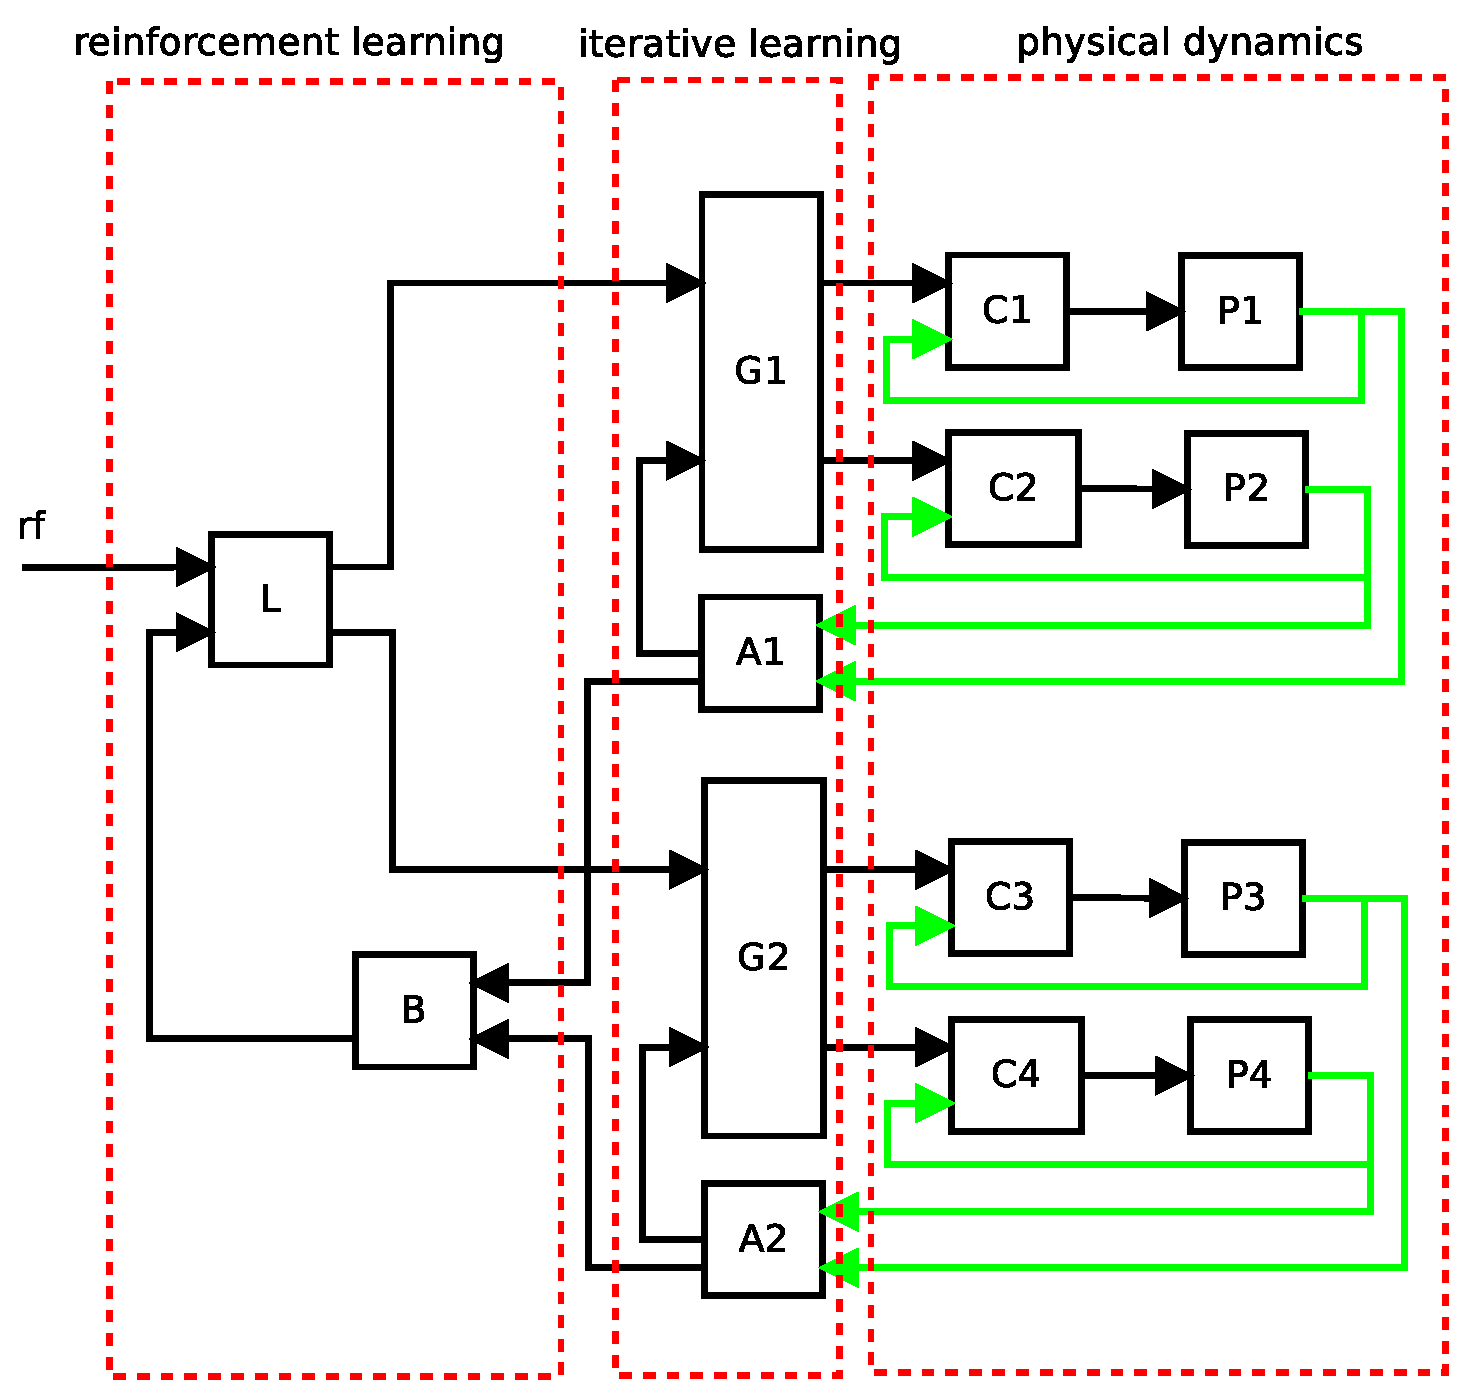
\includegraphics[scale=.5]{../diagrams/hierachical_system.eps}
\caption{Hierarchický systém riadenia}
\label{img:hierachical_controll_system}
\end{figure}

Obrázok je možné vysvetliť na príklade robotického ramena, so 4 stupňami voľnosti.
Cieľom je riadiť 4 sústavy $P1 \dots P4$, Na úrovni fyzikálnej vrstvy je možné použiť
adaptívne PID regulátory, do ktorých vstupuje výstup sústavy a požadovaná hodnota.
V prípade ramena je požadovanou hodnotou natočenie jednotlivých kĺbov. Tieto uhly sú
spočítané blokomi $G1$ a $G2$. Vstupom do regulátorov na fyzikálnej úrovni je tak
postupnosť uhlov generovaná blokomi $G1$ a $G2$. Na tejto úrovni sú zavedené aj
agregačné bloky $A1$ a $A2$, ktoré poskyjú $G$-blokom informáciu o stave systému.
Bloky $G$ spolu s regulátormi $C$ teda úspešne riešenia problém presunu ramena
po zadanej trajektórií.
Veľa systémom to postačuje - operatór výroby ľahko určí požadované trajektórie,
ktoré má robot vykonávať. V prípade komplexného problému, kedy požadované trajektórie
nie sú známe, má zmysel použiť blok $L$ - tretia úroveň, a nechať systém nech si trajektórie
a ich poradie určí sám. Používateľ systému do tohto procesu zasahuje odmeňovaním
alebo trestaním výsledného riešenia. Príkladom môže byť niekoľkokrová montáž výrobku.
Ktoré diely zložiť ako prvé, a ktoré ako posledné, aby bol výrobok zložený v čo najkratšom čase

triviálny príklad : osádzanie plošného spoja, osadiť najprv veľké alebo najprv malé súčiastky?
druhý príklad : šachy, vybudovať najprv obranu a stratiť niekoľko ťahov,
alebo sa radšej sústrediť na útok a riskovať slabinu vo vlastnej obrane?

V experimentálnej časti bude ako doplnková ukážka uvedený riadiaci mechanizmus robota
Motko Aftermath, sledujúceho čiaru kde sa požadovaná hodnota určuje predikciou pomocou neurónovej siete a
následne vstupuje do konvenčného regulátora \ref{img:motoko_reloaded}.

\begin{figure}[!htb]
\center
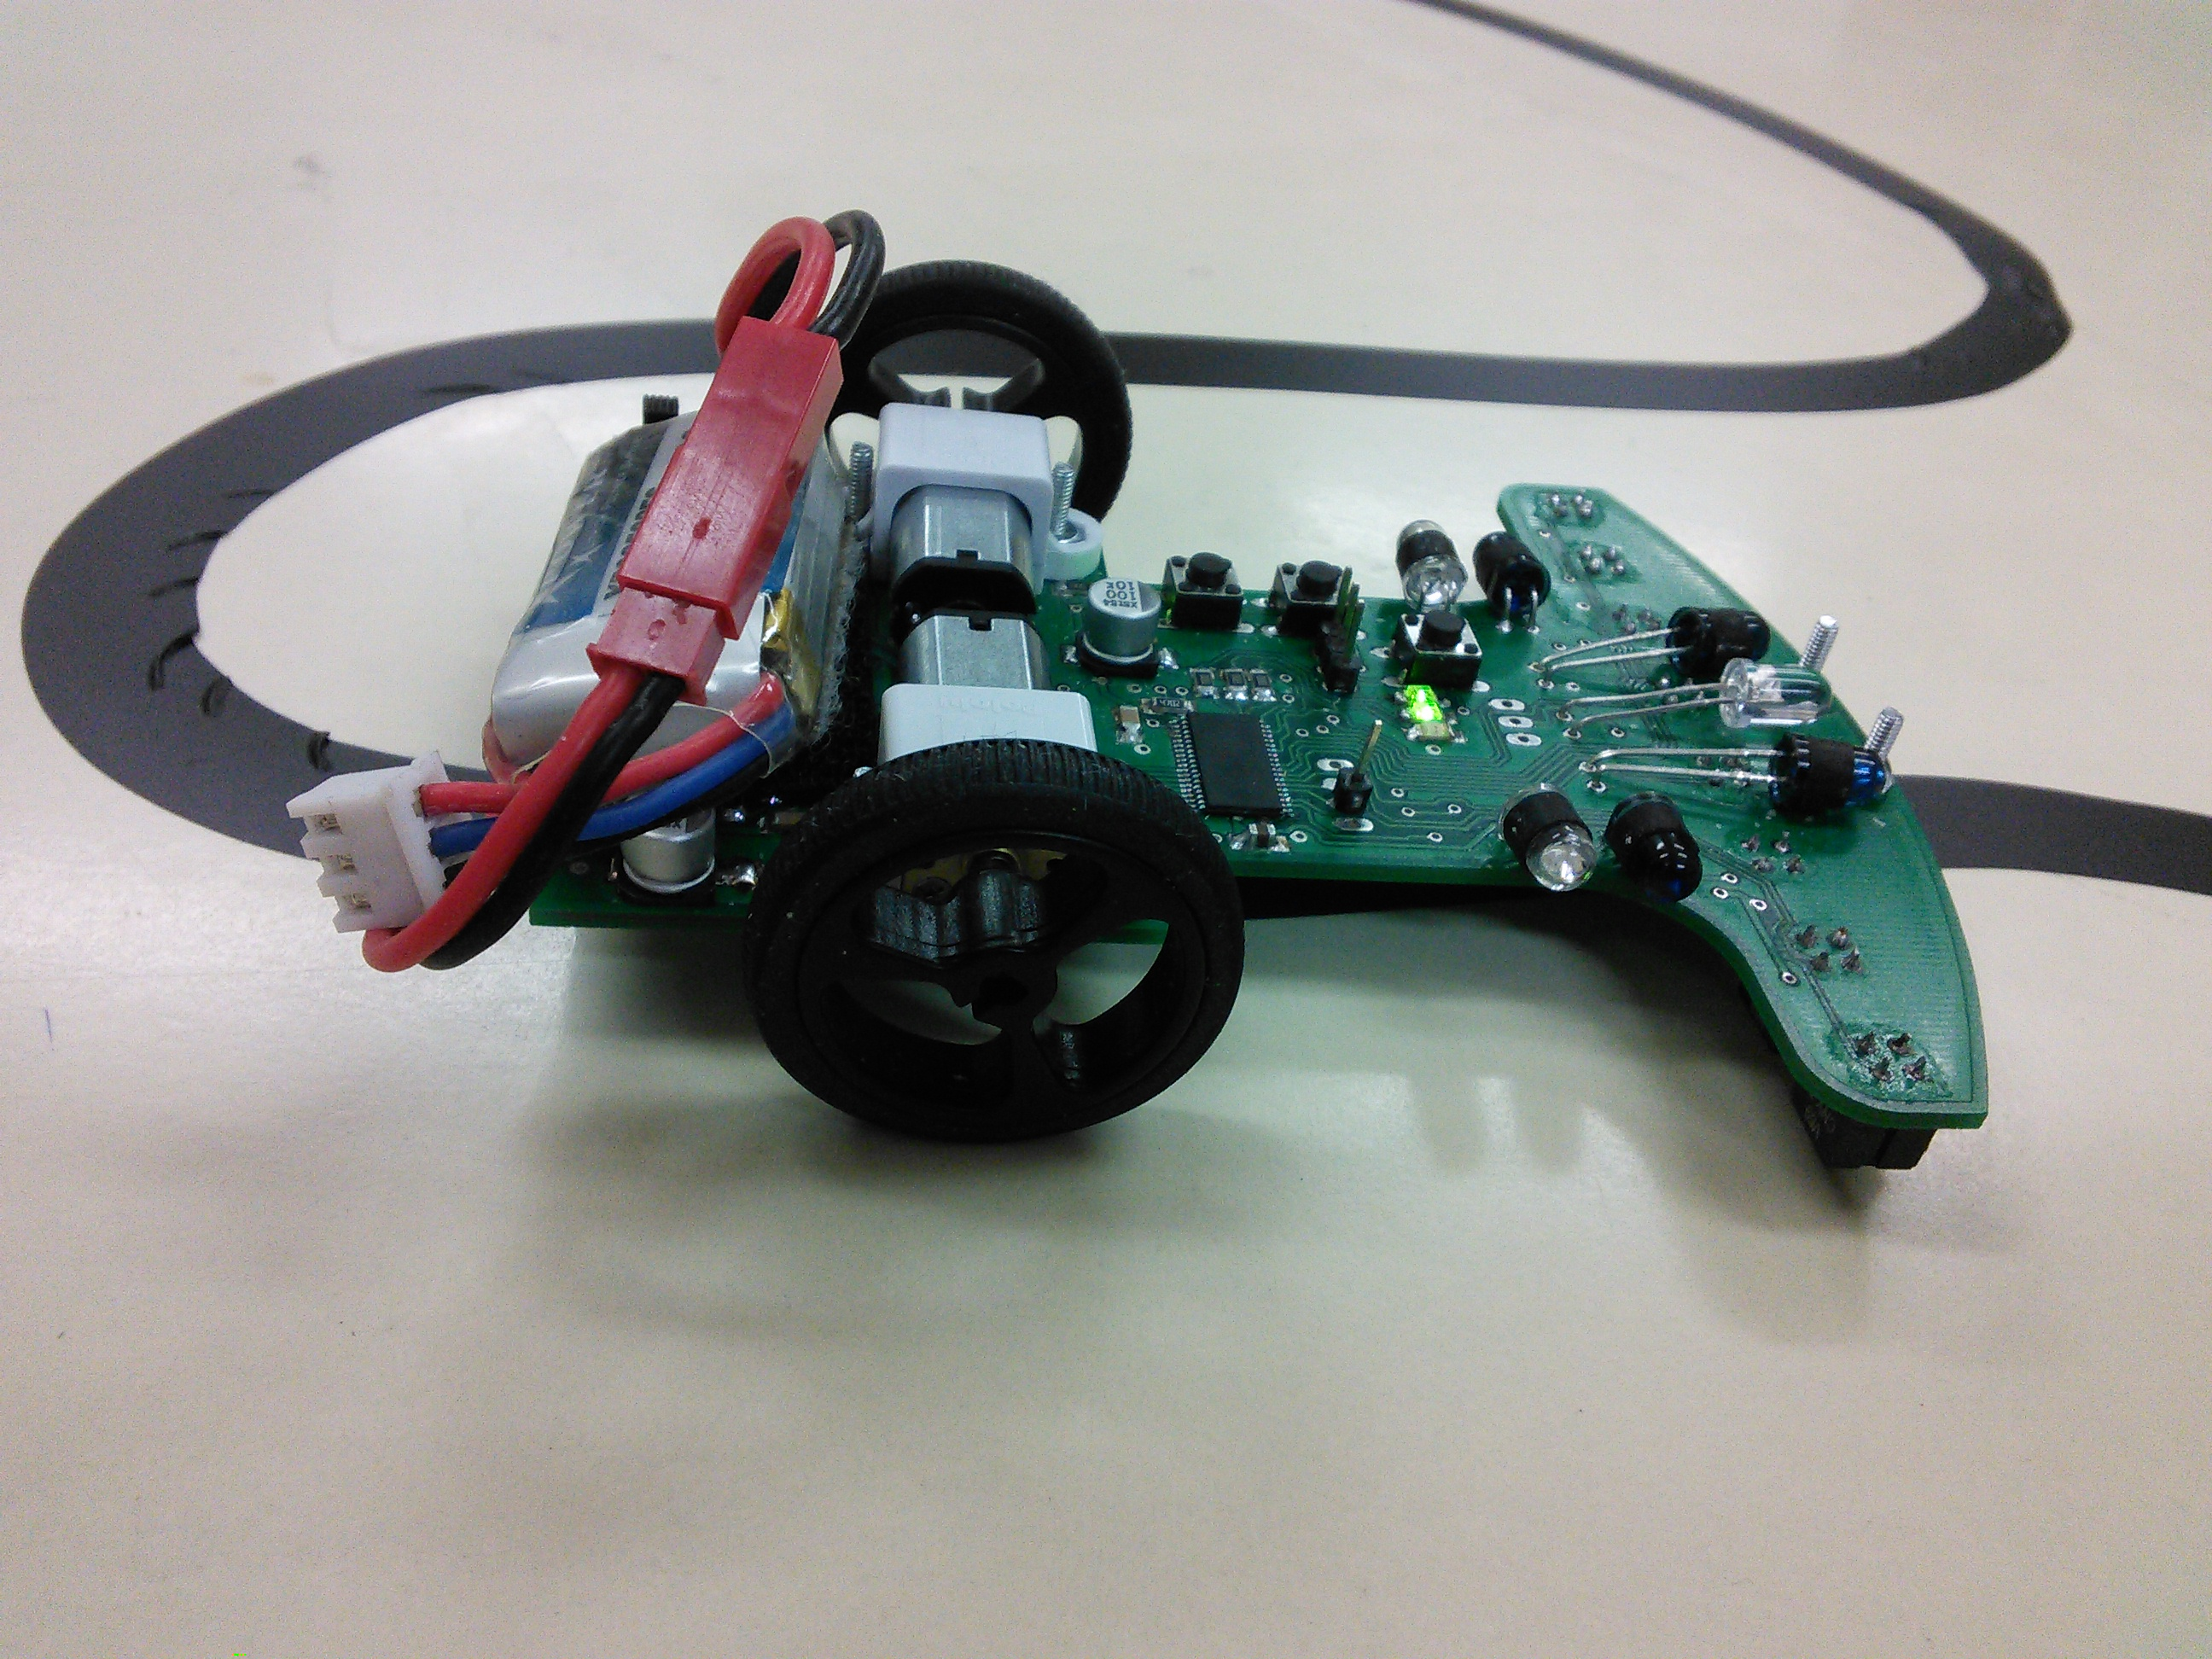
\includegraphics[scale=.1]{../pictures/motoko.jpg}
\caption{Ranná verzia robota}
\label{img:motoko_reloaded}
\end{figure}


\section{Markovove rozhodovacie procesy}


Množstvo úloh je možné popísať množinou stavov $\mathbb{S}$, pre každý stav je definovaná množina akcií
$\mathbb{A_S}$ \cite{bib:markov_01} \cite{bib:markov_02}. Pre každý stav a každú akciu, ktorú je v ňom možné vykonať existuje pravedepodobnostná
funkcia prechodu do ďalšieho stavu $P(s, s')$ a za uskutočnené prechody je daná funkcia odmien $R(s, s')$.
Formálne je teda Markovov proces pätica $(\mathbb{S}, \mathbb{A_S}, P(s, s'), R(s, s'), \gamma )$,
kde $\gamma \in (0, 1)$ je faktor zabúdania, a volí sa ako parameter procesu. Jeho význam bude vysvetlený
v ďalšej kapitole. Príklad Markovovho rozhodovacieho procesu je na obrázku \ref{img:markovov_decision_process}.
Prechody v grafe znamenajú jednotlivé akcie.

\begin{figure}[!htb]
\center
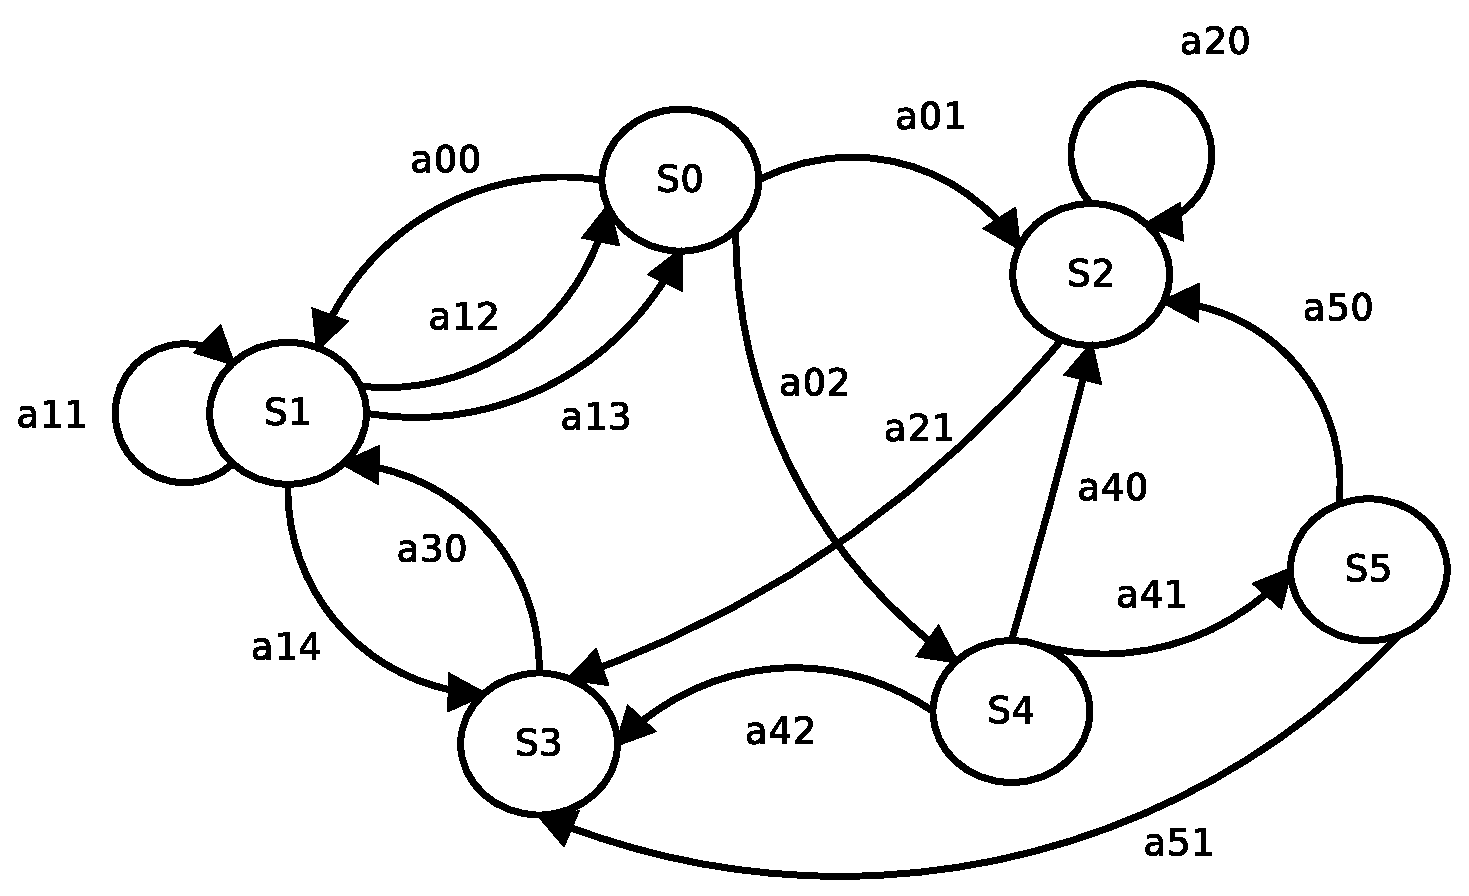
\includegraphics[scale=.5]{../diagrams/markovov_process.eps}
\caption{Markovov rozhodovací proces}
\label{img:markovov_decision_process}
\end{figure}

V priestore stavov $\mathbb{S}$ existuje výkonná jednotka - agent. Je to modul
ktorý na základe vstupnej informácie - stave vyberie jednu z akcií. To s akou pravdepodobnosťou
sa daná akcia vykoná je dané prostredím (popísané Markovove rozhodovacím procesom).

Dôležitým východiskom je, že $P(s, s')$ nie je agentovi známa. Agent teda nemôže
vedieť kam sa vykonaním vybranej akcie dostane. Tento fakt značne komplikuje prehľadávanie
priestoru.
Ďalším typickým rysom je, že odmeňovacia funkcia $R(s, s')$, ktorá je zadaná,
nadobúda pre väčšinu prechodov z $s$ do $s'$ hodnotu 0. Je to dôsledok prirodzeného
spôsobu riešenia problémov delením na čiastkové kroky a nie je okamžite známa
veľkosť úžitku po vykonaní čiastkového kroku. Často je táto skutočnosť známa
len pre pár vybraných prechodov.
Dobrým príkladom tejto situácie je hra Go.

\begin{figure}[!htb]
\center
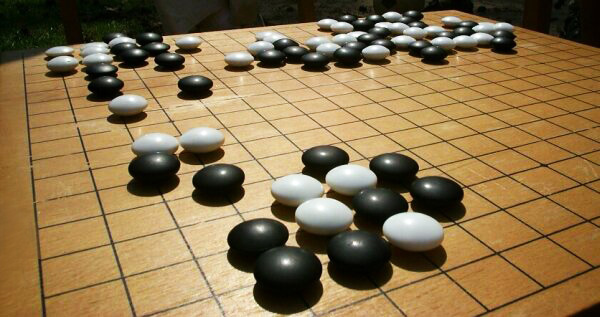
\includegraphics[scale=.5]{../pictures/go2.jpg}
\caption{Hra Go}
\label{img:go_game}
\end{figure}

Položením kameňa na Goban nie okamžite známe ako to ovplyvní priebeh hry.
Je bežné, že sa to prejaví až po mnohých krokoch.




















\section{Adaptívny systém}

V teorií riadenia sa narába s pojmami spätná väzba, žiadaná hodnota,
chybová veličina, riadená sústava, regulátor a model. Obrázok \ref{img:adaptive_controll_system} zobrazuje
prepojenie základných blokov typického adaptívneho systému.


\begin{figure}[!htb]
\center
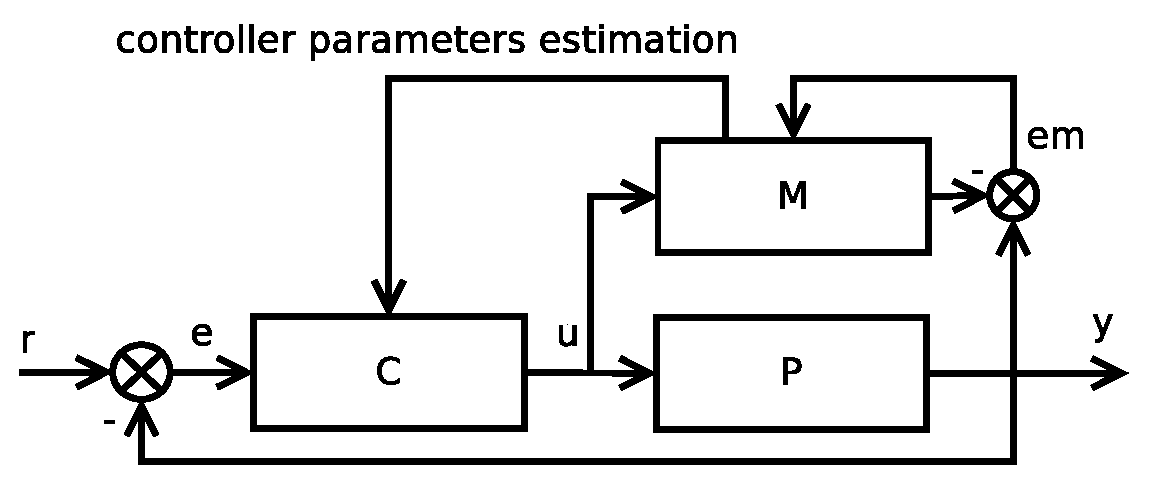
\includegraphics[scale=.6]{../diagrams/adaptive_system.eps}
\caption{Adaptívny riadiaci systém}
\label{img:adaptive_controll_system}
\end{figure}

Pre ďalšie účely sa bude hovoriť o systémoch pracujúcich v diskrétnom čase $n$ s
krokom $1$. Vstupom je žiadaná hodnota $r(n)$, výstupom je $y(n)$. Z toho nevyhnutne
vyplýva definícia chybovej veličiny ako $e(n) = r(n) - y(n)$.
Kvalitu regulátora je možné definovať rôznymi spôsobmi, najbežnejší je

\begin{equation}
K = \sum\limits_{n=1}^{\infty}{e(n)^2}
\label{eq:controller_quality}
\end{equation}

Cieľom je minimalizovať $K$. Je možné definovať aj ďalšie kritéria,
ako doba ustálenia a veľkosť najväčšieho prekmitu.

Regulátor $C(n)$ je blok, tvorený obvykle diferenčnou rovnicou s volenými
parametrami do ktorého vstupuje chyba.
Veličina $u(n)$ je výstup regulátora a nazýva sa akčná veličina, predstavuje
vstup do riadenej sústavy $C(n)$. Akčná veličina ďalej vstupuje do modelu systému
ktorého parametre sa menia podľa chyby modelu $e_m(n) = y(n) - y_m(n)$, kde $y_m(n)$
je výstup modelu. Cieľom je minimalzovať $L(c) = \sum\limits_{n=1}^{c}{{e_m}(n)^2}$.
Po dosiahnutí minima sa parametre modelu rovnajú parametrom riadenej sústavy,
a je tak možné urobiť syntézu regulátora.


\section{Princípy učenia s odmneňovaním}

Pre všetky $n$ musí existovať požadovaná hodnota $r(n)$ a k nej prislúchajúca
chyba $e(n)$. Čo v prípade systémov kedy nie je pre všetky $n$ definované správanie?
Príkladom môže byť rozhodovanie robota, ktorý má splniť ciel pozostávajúci z
niekoľkých elementárnych úkonov, ale postupnosť týchto elementárnych úkonov nie je známa -
nie je teda definované $r(n)$ pre kazdé $n$.

Riešením tohto problému je zavedenie systému odmeňovania agenta (robota) \ref{img:reinforcement_learning}.

\begin{figure}[!htb]
\center
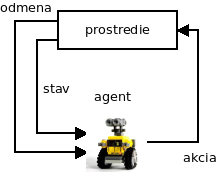
\includegraphics[scale=.8]{../diagrams/agent.png}
\caption{Učenie s odmeňovaním}
\label{img:reinforcement_learning}
\end{figure}

Táto metóda sa nazýva  {\bf reinforcement learning}. V súčastnosti predstavuje
najmocnejší nástroj strojového učenia v oblasti umelej inteligencie. Umožňuje
riešiť veľmi komplexné problémy a uplatnenie nachádza nie len v počítačových
hrách, ale napr. aj v robotike.
Jej princíp je možné zhrnúť do týchto bodov :

\begin{enumerate}
  \item Zistenie stavu
  \item Výber akcie
  \item Vykonanie akcie
  \item Prechod do ďalšieho stavu
  \item Získanie odmeny alebo trestu
  \item Učenie sa zo získanej skúsenosti
\end{enumerate}

 {\bf Zistenie stavu} je umožnené vnímaním prostredia, napr. pomocou senzorov.
V najjednoduhšom prípade si je možné ako stav predstaviť polohu. Vo
všeobecnosti, to ale nemusia byť ani priamo dáta so vstupov, ale len nejaké
príznaky - robot je na križovatke $p_0 = 0.9$, robot je v uličke $p_1 = 0.3$ .
Sada príznakov umožňuje zredukovať dimenziu stavového priestoru (tá musí
byť pre ďalej rozoberané algoritmy konečná, vyplynie to z prezentovaných rovníc).

{\bf Výber akcie} je uskutočnený na základe ohodnotení akcií získanych
v minulosti. Tieto ohodnotenia sú samozrejme závislé od stavu v ktorom sa
systém nachádza - tá ista množina akcií má iné ohodnotenie keď je robot na
križovatke a iné keď je v uličke. Vo fáze prieskumu prostredia môže agent
vyberať tie akcie ktoré boli v minulosti málo často vykonané, alebo môže vyberať náhodne.
Definovaním veľkosti zmeny ohodnotenia akcie môže uprednostniť tie akcie,
ktorých ohodnotenia vykazujú veľkú zmenu - pretože je pravdepodobné že sa
tým dostane do nepreskúmaných stavov.
Vo fáze kedy agent už nepreskúmavá prostredie, môže vyberať len najlepšie ohodnotenú akciu.
Prípadne môžu existovať v prostredí s viacerími agentami prieskumníci a vykonávatelia.
Navzájom si môžu vymieňať skúsenosti.

{\bf Vykonanie akcie} V deterministickom prostredí sa vybraná akcia vykoná vždy rovnako
(opäť však závisí na stave agenta). V nedeterministickom prostredí sa vykonanie
sa akcie riadi nejakou pravdepodobnostnou funkciou - napr. robotovi môže prešmyknúť
koleso.

{\bf Prechod do ďalšieho stavu} je obvyklým dôsledkom vykonania akcie. Samozrejme, že
v danom stave môže existovať aj taká akcia ktorá nespôsobí zmenu stavu - napr. spomínané
prešmyknutie kolesa - robot sa nepohne.

{\bf Získanie odmeny alebo trestu} po vykonaní akcie, existuje odmeňovací mechanizmus
zadaný tvorcom systému. Preto sa nedá hovoriť o umelej inteligencií - správanie
sa agenta je v deterministickom prostredí plne určené týmto mechanizmom - len nie je známe.
Obvykle platí, že kladné hodnoty dosahuje odmena, záporné trest. Nulová hodnota symbolizuje
neznalosť zadavateľa, a nevie teda určiť či dané konanie bolo dobré alebo zlé.
Nesmierne dôležitý je fakt, že pre veľkú väčšinu rozhodnutí je výsledkom odmeny práve nula.
Príkladom môže byť japonská hra Go - pre úspešné vedenie partie nestačí ohodnotiť
len aktuálny stav na gobane, je potrebné uvažovať viac ťahov dopredu - úspešnosť
ťahu sa často ukáže až po vykonaní množstva ďalších ťahov, kedy je odmena už nenulová.

Práve dominancia nulových odmien je unikátom pre reinforcement learning algoritmy.
Od zadávateľa sa vyžaduje minimum znalostí, je dokonca možné ukázať, že stačí
odmena len v cieľovom stave (i keď proces učenia bude v tomto prípade trvať veľmi dlho).


\section{Ohodnocovanie vykonaných akcií}

Odmena je získaná z prostredia po vykonaní akcie. Ohodnotenie akcie v danom stave
je tvorené predoslými skúsenosťami z vykonania predošlých akcií a získania odmien.
Podstatou učenia je teda ohodnotenie vykonaných akcií v danom stave, aby bolo
možné v každom stave rozhodnúť ktorá akcia je najlepšia - vyberá sa teda
postupnosť akcií $\pi$ pre ktorú je funkcia

\begin{equation}
\Lambda(\pi)  = \sum\limits_{n=0}^{\infty}\gamma^n R_{\pi(n)}(s(n), s(n-1))
\label{eq:q_quality}
\end{equation}

maximálna. Kde $\gamma \in \langle 0, 1 \rangle$ je koeficient zabúdania, $R_{\pi(n)}{(s(n), s(n-1)}$
je odmeňovacia funkcia po prechode zo stavu $s(n-1)$ do stavu $s(n)$ vykonaním $\pi(n)$.

Hľadanie mechanizmu nájdenia maxima $\Lambda(\pi)$ bude vysvetlené na nasledujúcich príkladoch.
\\
Pre ilustráciu bude postupnosť prechodov zapísaná priamo ako prameter funkcie $\Lambda$, napr :
$\Lambda(\{S_0, S_7, S_5\})$ predstavuje prechody z $S_0$ do $S_7$ a z $S_7$ do $S_5$.
Ďalej sa predpokladá že $\gamma = 1$.
\\
Je daný systém s troma stavmi, a dvoma prechodmi \ref{img:three_states_system}.
Pre ilustráciu je systém tak jednoduchý, že každá akcia má známu odmenu.

\begin{figure}[!htb]
\centering
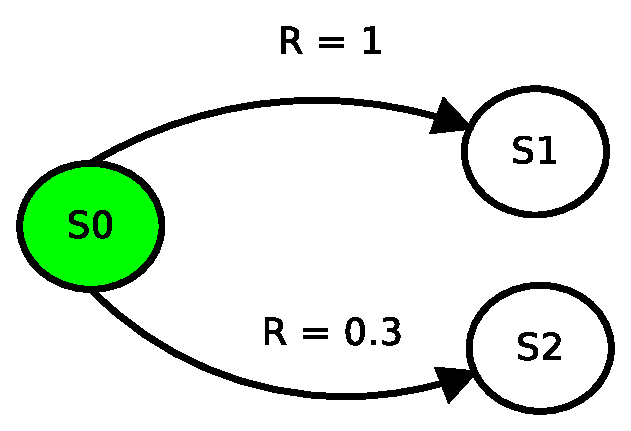
\includegraphics[scale=.6]{../diagrams/rf_two_states.eps}
\caption{Ohodnocovanie akcií v trojstavom systéme}
\label{img:three_states_system}
\end{figure}

V tomto systéme je ohodnotenie $\Lambda(S_a, S_b)$ naozaj triviálne

\begin{enumerate}
  \item $\Lambda(\{S_0, S_1\}) = 1$
  \item $\Lambda(\{S_0, S_1\}) = 0.3$
\end{enumerate}

Najlepšia cesta je potom $\{S_0, S_1\}$.

V prípade systému s viacerými stavmi \ref{img:multiple_states_system}, ale
opať známimi ohodnoteniami v každom prechode bude situácia nasledovná.

\begin{figure}[!htb]
\centering
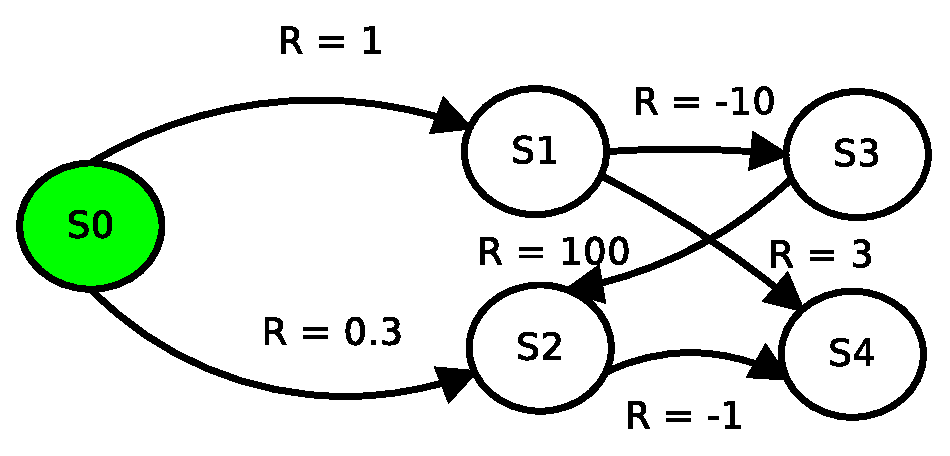
\includegraphics[scale=.6]{../diagrams/rf_more_states.eps}
\caption{Ohodnocovanie vo viacstavovom systéme}
\label{img:multiple_states_system}
\end{figure}

Ohodnotenie ciest :
\begin{enumerate}
  \item $\Lambda(\{S_0, S_1, S_3\}) = 1+(-10) = -9$
  \item $\Lambda(\{S_0, S_1, S_4\}) = 1+3 = 4$
  \item $\Lambda(\{S_0, S_2, S_4\}) = 0.3 +()-1) =-0.7$
  \item $\Lambda(\{S_0, S_1, S_3, S_2, S_4\}) = 1 +(-10) +100 + (-1) = 90$
  \item ...
\end{enumerate}

Jednoduchých ščítaním ohodnotení rôznych ciest je tak možné nájsť optimálnu
postuponosť akcií.

Ak sa v systéme nachádza cyklus \ref{img:cycle_states_system} (na obrázku
je triviálny prípad) ohodnotenie bude divergovať. Agent bude mať možnosť
vykonávať akciu ktorá neustále pripočítava kladnú odmenu, nevyhnutne tak
vyberie túto stratégiu, pretože tak získa nekonečne veľkú odmenu.

\begin{figure}[!htb]
\centering
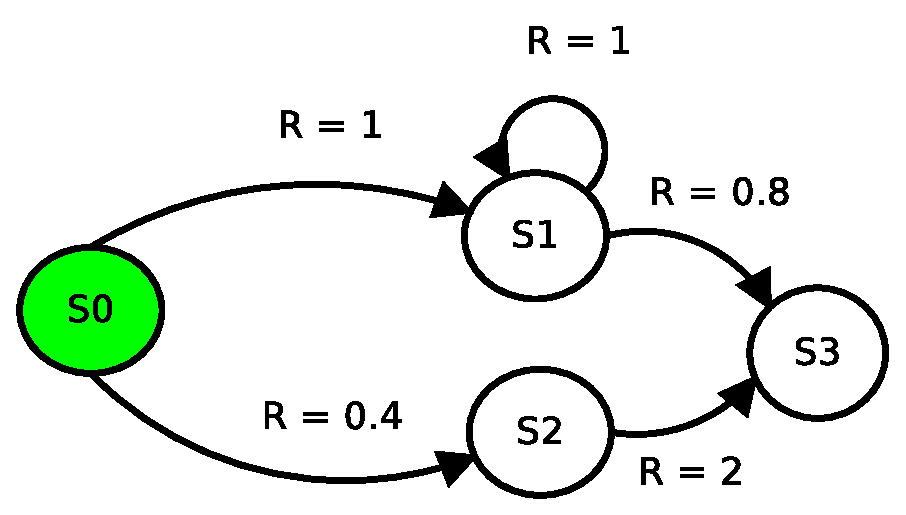
\includegraphics[scale=.6]{../diagrams/rf_cycle_states.eps}
\caption{Ohodnocovanie s cyklom}
\label{img:cycle_states_system}
\end{figure}

Ohodnotenie niektorých ciest
\begin{enumerate}
  \item $\Lambda(\{S_0, S_2, S_3\}) = 0.4+2 = 2.4$
  \item $\Lambda(\{S_0, S_1, S_3\}) = 1+1 = 2$
  \item $\Lambda(\{S_0, S_1, S_1, S_1\}) = 1+1+1 = 3$
  \item $\Lambda(\{S_0, S_1, S_1, S_1, S_1\}) = 1+1+1+1 = 4$
  \item $\Lambda(\{S_0, S_1, S_1, S_1, S_1, S_1, ...\}) = 1+1+1+1+1+...+1 = \infty$ !!!!
\end{enumerate}

Riešením je práve zavedenie faktora zabúdania $\gamma$. Ilustračne
bola zvolená $\gamma = 0.9$. Agent tak síce urobí niekoľko cyklov $S_1, S_1$,
po čase ale hodnota odmeny konverguje a minulé príspevky dávajú čoraz menší
a menší úžitok a nevyhnutne tak po niekoľkých cyklov zmení rozhodnutie a prejde
z $S_1$ do $S_3$.

Ohodnotenie niektorých ciest
\begin{enumerate}
  \item $\Lambda(\{S_0, S_2, S_3\}) = 2 + 0.9*0.4 = 2.36$
  \item $\Lambda(\{S_0, S_1, S_3\}) = 1 + 0.9*1 = 1.9$
  \item $\Lambda(\{S_0, S_1, S_1, S_1\}) = 1 + 0.9*(1 + 0.9*1) = 2.71 $
  \item $\Lambda(\{S_0, S_1, S_1, S_1, S_1\}) = 1 + 0.9*(1 + 0.9*(1 + 0.9*1)) = 3.439$
  \item $\Lambda(\{S_0, S_1, S_1, S_1, S_1, S_1, ...\}) = 10$ <-----
  \item $\Lambda(\{S_0, S_1, S_1, S_1, S_1, S_1, ..., S3\}) = 11$ <-----
\end{enumerate}

Cyklovanie v $S_1$ teda prinesie celkovú odmenu 10, ale pri prechode do $S_3$ je celková
odmena 11.

Formálny prepis uvedených úvah vedie na Q-learning algoritmus, ktorý zohľadňuje Bellmanov princíp optimality.


\section{Jednostavový systém}

Prv než bude uvedené úplne znenie Q-learning algoritmu je vhodné rozobrať ešte
jeden príklad, a to systém s jedným stavom \ref{img:single_state_system}.
Tento problém vznikol z nasledujúcej úvahy : je daný robot ktorý má jeden senzor
vzdialenosti od cieľa (nevie teda určiť smer (napr. senzor intenzity osvetlenia) ) a možnosti pohybu o elementárny krok
vpred, vľavo, vpravo, vzad. Ako zvoliť postupnosť akcií aby robot došiel do cieľa - minimalizoval vzdialenosť?
Navyše sa predpokladá, že senzor je nekvalitný a záludný zároveň : poskytuje
informáciu len o tom či sa situácia zlepšila alebo zhoršila (oproti predošlému meraniu),
a s určitou pravdepodobnosťou generuje náhodnú hodnotu - náhodné zmení výsledok (šum).

To vedie na zostavenie odmeňovacej funkcie ako

\begin{equation}
R(n) =
\left\{
	\begin{array}{ll}
		k  & ak \ d(n) - d(n-1) < 0 \\
    -k & inak
	\end{array}
\right.
\label{eq:q_nano_r_func_simple}
\end{equation}

kde $d(n)$ je zmeraná vzdialenosť a na $d(n) - d(n-1) < 0 $ sa pozerá
ako uzavretú časť - vstupon do algoritmu teda nie je samotné $d(n)$ ale až
$R(n)$. Pre $k$ platí : $k = 1 \ ak \ rnd(0, 1) > p \ , inak \ -1$, kde $p$ je pravdepodobnosť
zmeny nameranej hodnoty $p \in \langle 0, 1 \rangle $ a $rnd(0, 1)$ generuje náhodné
číslo z intervalu $\langle 0, 1 \rangle$.

\begin{figure}[!htb]
\centering
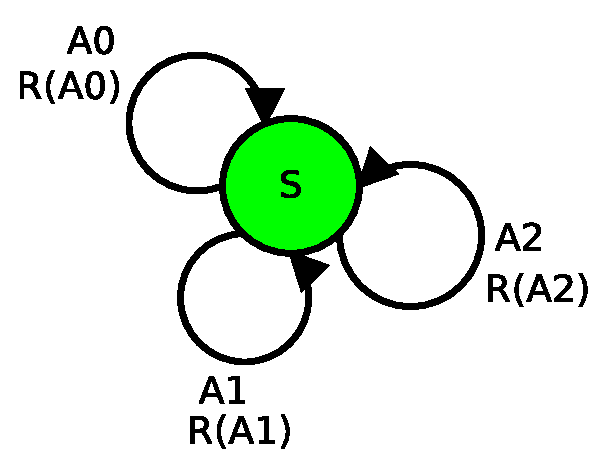
\includegraphics[scale=.6]{../diagrams/single_state.eps}
\caption{Jednostavový systém s troma akciami}
\label{img:single_state_system}
\end{figure}

Kľúčový je výber akcie $a(n)$ z konečnej množiny akcií $\mathbb{A}$,
vychádza sa z predstavy : ak má vykonaná akcia dobré ohodnotenie,
vykoná sa znova, ak má zlé ohodnotenie, vyberie sa iná, náhodná akcia.
Formálne zapísané

\begin{equation}
a(n) =
\left\{
	\begin{array}{ll}
		a(n-1)  & ak \ Q_{n-1}(a(n-1)) > 0 \\
    random() & inak
	\end{array}
\right.
\label{eq:q_nano_action_selection}
\end{equation}

Samotné $Q$ predstavujúce ohodnotenie sa potom vypočíta ako

\begin{equation}
Q_n(A(n)) = R(n) + \gamma  \max_{a'(n-1) \in \mathbb{A}} Q_{n-1}(a'(n-1))
\label{eq:nano_q_func}
\end{equation}

Algoritmus je teda veľmi jednoduchý a možno ho použit na plánovanie pohybu robota.
Robotovi tak nie vnútené správanie programátorom, ale sám sa naučí ktoré akcie
vyberať.


\subsection{Výsledky experimentu}

Overenie prebehlo s 32 virtuálnymi robotmi. Cieľom bolo naháňať pohyblivý cieľ,
ktorý sa pohyboval po kružnici. Počiatočné polohy robotov boli náhodné.
Celý experiment prebiehal v dvojrozmernom priestore obmedzenom na rozsah
polohy $\langle -1, 1 \rangle$. Metrika vzdialenosti bola Euklidovská.

Po 25000 iteráciach sa počítala priemerná chyba z 32 robotov. Vyšetrovala
sa závislosť tejto chyby od zmeny parametrov $\gamma$ a $p$ (na grafe ako gamma a noise).
Pre vybrané prípady boli exportované aj dráhy prvých 8 robotov.

Prostredie sa tak postupne mení z plne deterministického bez šumu až po hodnotu $0.4$,
čo predstavuje $40\%$ pravdepodobnosť zmeny hodnoty senzora. Graf závislosti priemernej chyby
od parametrov $\gamma$ a $p$ je na obrázku \ref{img:nano_q_summary}.

\begin{figure}[!htb]
\centering
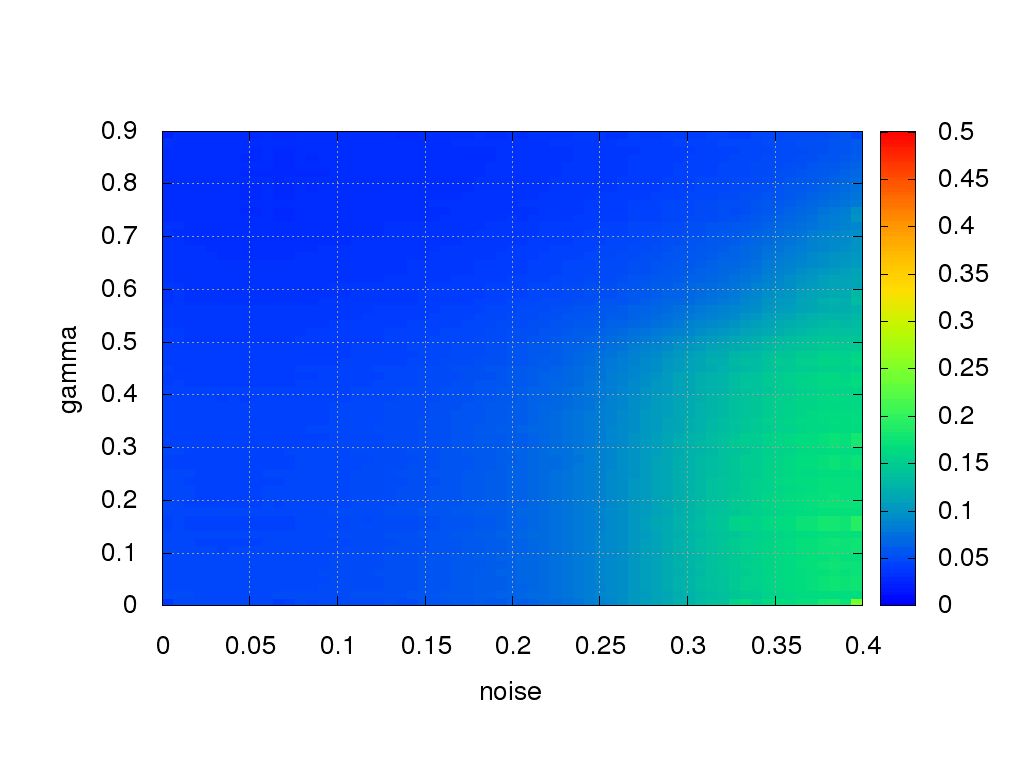
\includegraphics[scale=.4]{../../results_q_learning/nano_q_learning/summary_result_average_error_map.png}
\caption{Priemerná chyba 32 robotov po 25000 iteráciach}
\label{img:nano_q_summary}
\end{figure}

Dráhy robotov pre niektoré zvolené parametre sú uvedené v tabuľke \ref{tab:nano_q}

\begin{center}
  \begin{tabular}{ | c | c || c | c |}
    \hline
    $\gamma$ & $p$ & graf dráhy & graf vývoja chyby \\ \hline
    $0.7$ & $0.0$ & \ref{img:nano_q_result_00_path} & \ref{img:nano_q_result_00_error} \\
    $0.7$ & $0.3$ & \ref{img:nano_q_result_03_path} & \ref{img:nano_q_result_03_error} \\
    $0.0$ & $0.4$ & \ref{img:nano_q_result_04_1_path} & \ref{img:nano_q_result_04_1_error} \\
    $0.7$ & $0.4$ & \ref{img:nano_q_result_04_2_path} & \ref{img:nano_q_result_04_2_error} \\
    $0.9$ & $0.4$ & \ref{img:nano_q_result_04_3_path} & \ref{img:nano_q_result_04_3_error} \\
    $0.98$ & $0.4$ & \ref{img:nano_q_result_04_4_path} & \ref{img:nano_q_result_04_4_error} \\
    \hline
    \end{tabular}
    \captionof{table}{Vybrané parametre experimentu a odkaz na grafické znázornenie výsledku}
    \label{tab:nano_q}
\end{center}

\begin{figure}[!htb]
\centering
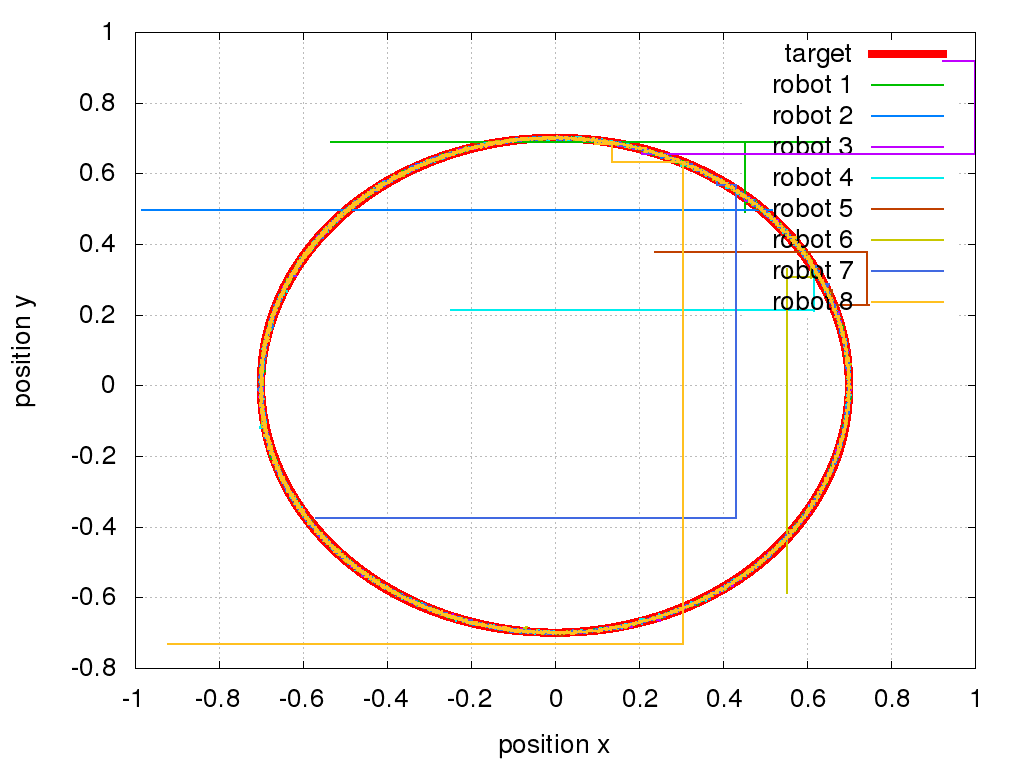
\includegraphics[scale=.4]{../../results_q_learning/nano_q_learning/result_00/robot_path.png}
\caption{Dráha robotov pre $\gamma = 0.7 p = 0.0$}
\label{img:nano_q_result_00_path}
\end{figure}

\begin{figure}[!htb]
\centering
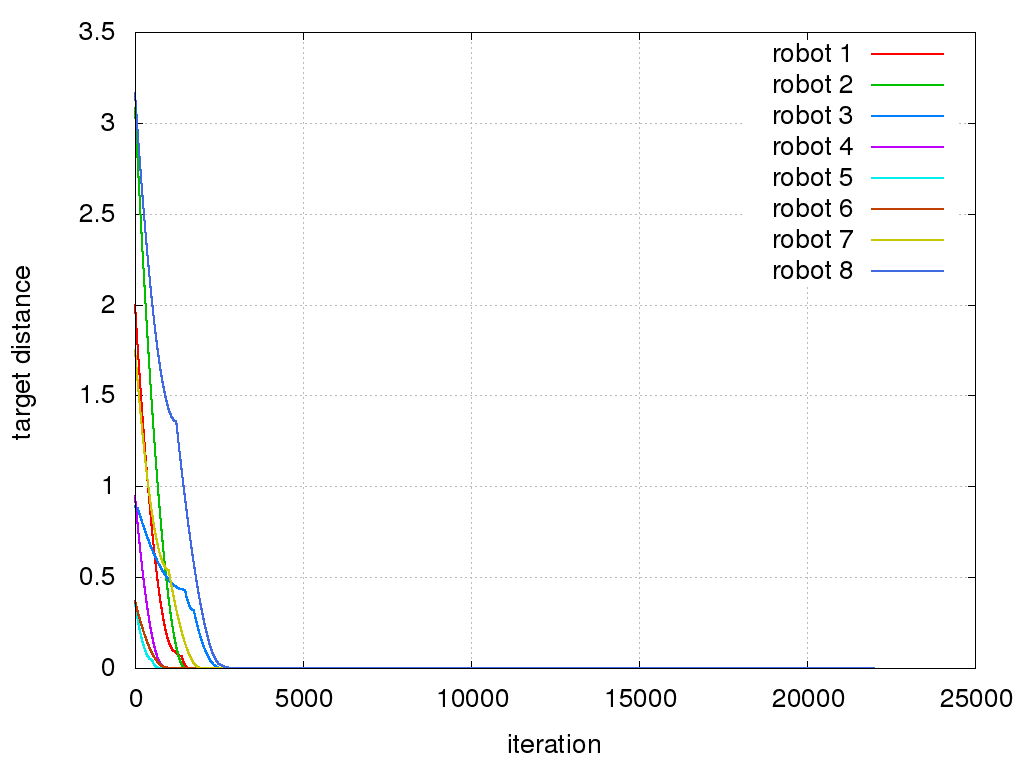
\includegraphics[scale=.4]{../../results_q_learning/nano_q_learning/result_00/robot_reward.png}
\caption{Vzdialenosť robotov od cieľa pre $\gamma = 0.7 p = 0.0$}
\label{img:nano_q_result_00_error}
\end{figure}



\begin{figure}[!htb]
\centering
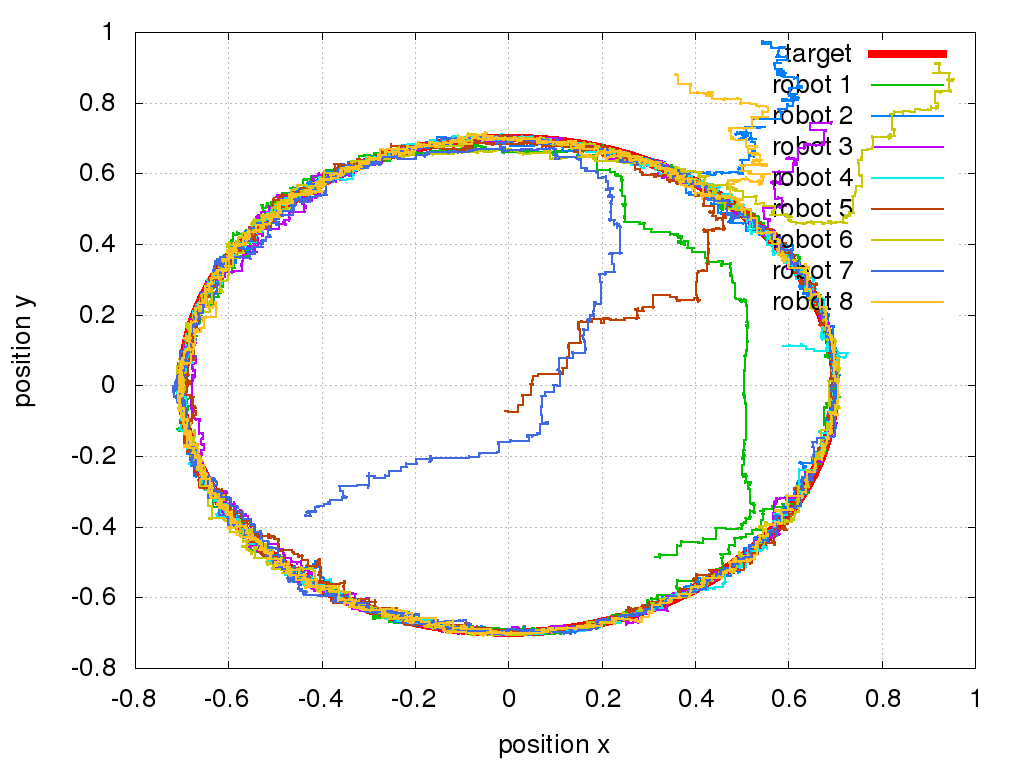
\includegraphics[scale=.4]{../../results_q_learning/nano_q_learning/result_03/robot_path.png}
\caption{Dráha robotov pre $\gamma = 0.7 p = 0.3$}
\label{img:nano_q_result_03_path}
\end{figure}

\begin{figure}[!htb]
\centering
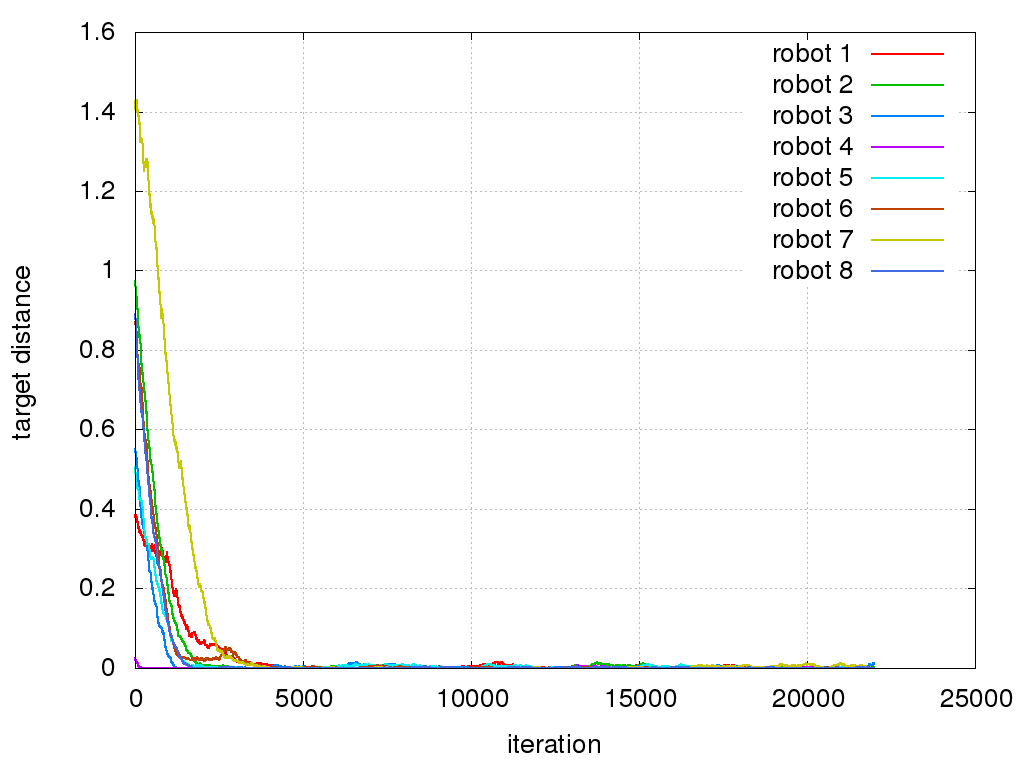
\includegraphics[scale=.4]{../../results_q_learning/nano_q_learning/result_03/robot_reward.png}
\caption{Vzdialenosť robotov od cieľa pre $\gamma = 0.7 p = 0.3$}
\label{img:nano_q_result_03_error}
\end{figure}



\begin{figure}[!htb]
\centering
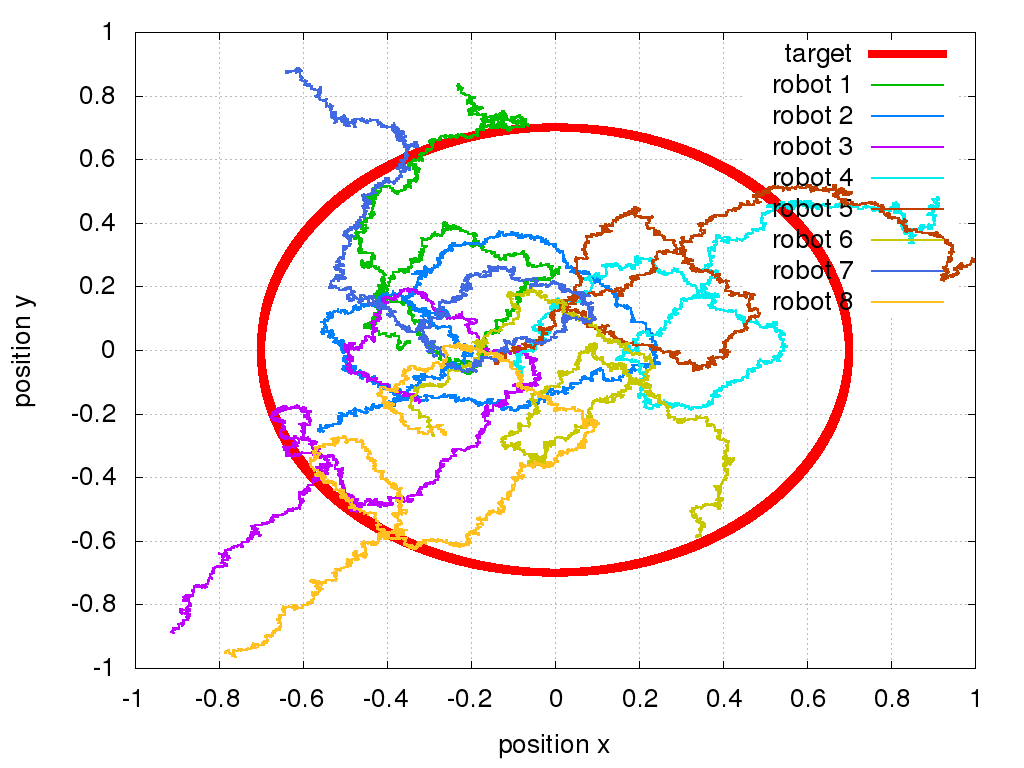
\includegraphics[scale=.4]{../../results_q_learning/nano_q_learning/result_04_01/robot_path.png}
\caption{Dráha robotov pre $\gamma = 0.0 p = 0.4$}
\label{img:nano_q_result_04_1_path}
\end{figure}

\begin{figure}[!htb]
\centering
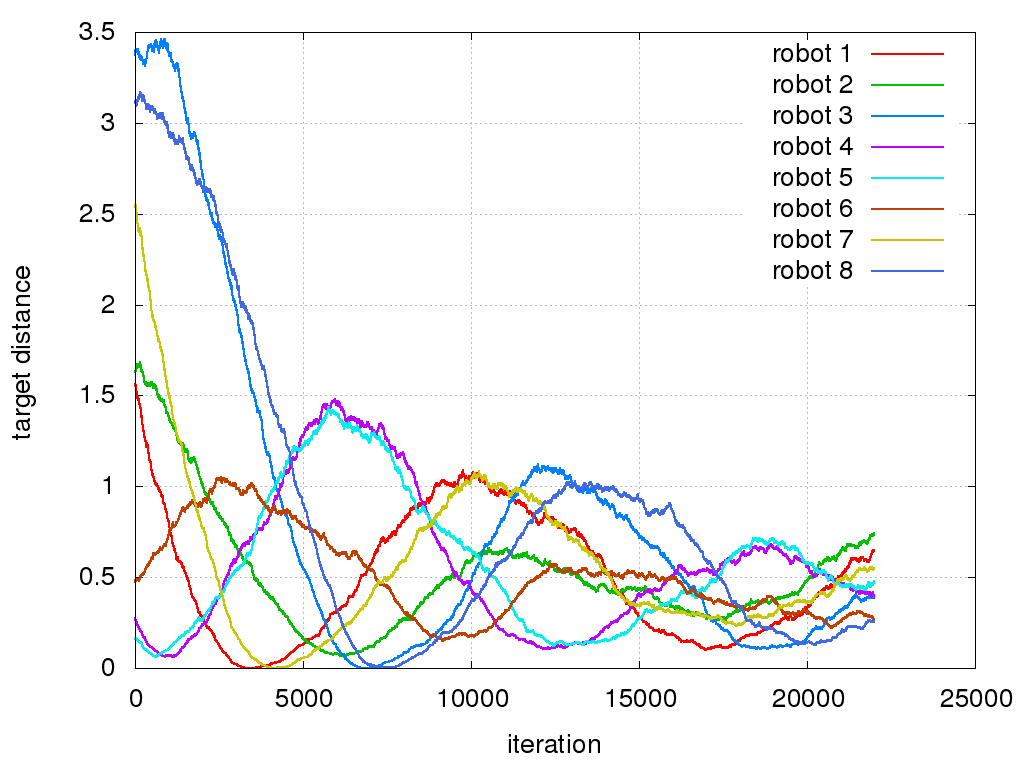
\includegraphics[scale=.4]{../../results_q_learning/nano_q_learning/result_04_01/robot_reward.png}
\caption{Vzdialenosť robotov od cieľa pre $\gamma = 0.0 p = 0.4$}
\label{img:nano_q_result_04_1_error}
\end{figure}




\begin{figure}[!htb]
\centering
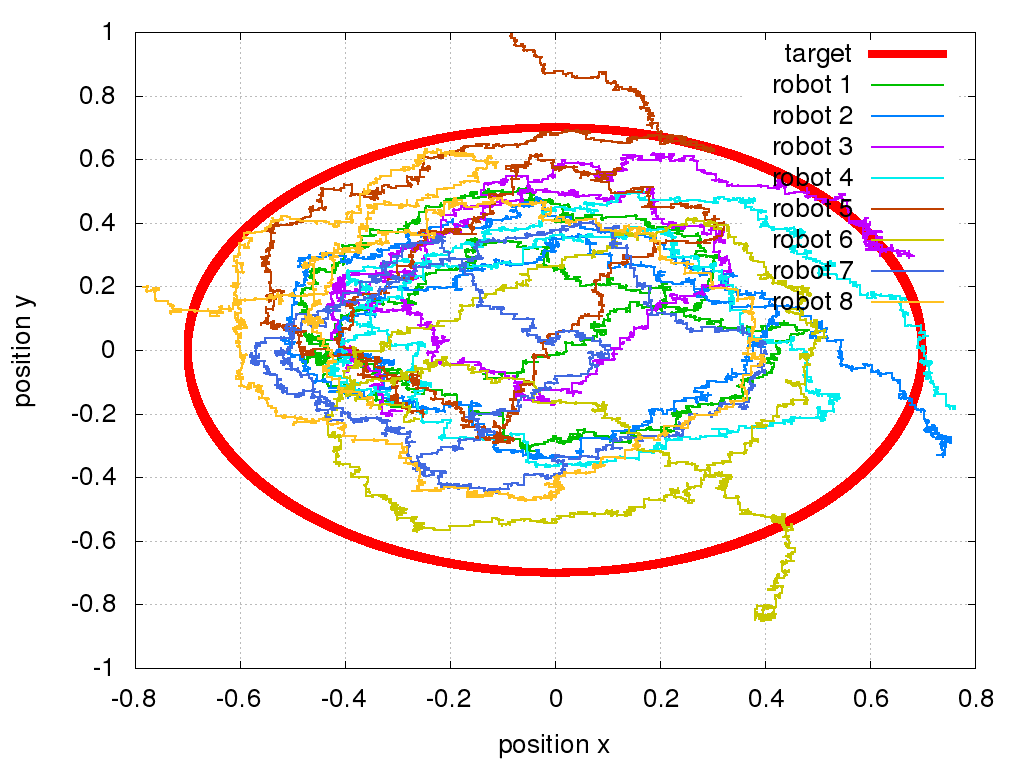
\includegraphics[scale=.4]{../../results_q_learning/nano_q_learning/result_04_02/robot_path.png}
\caption{Dráha robotov pre $\gamma = 0.7 p = 0.4$}
\label{img:nano_q_result_04_2_path}
\end{figure}

\begin{figure}[!htb]
\centering
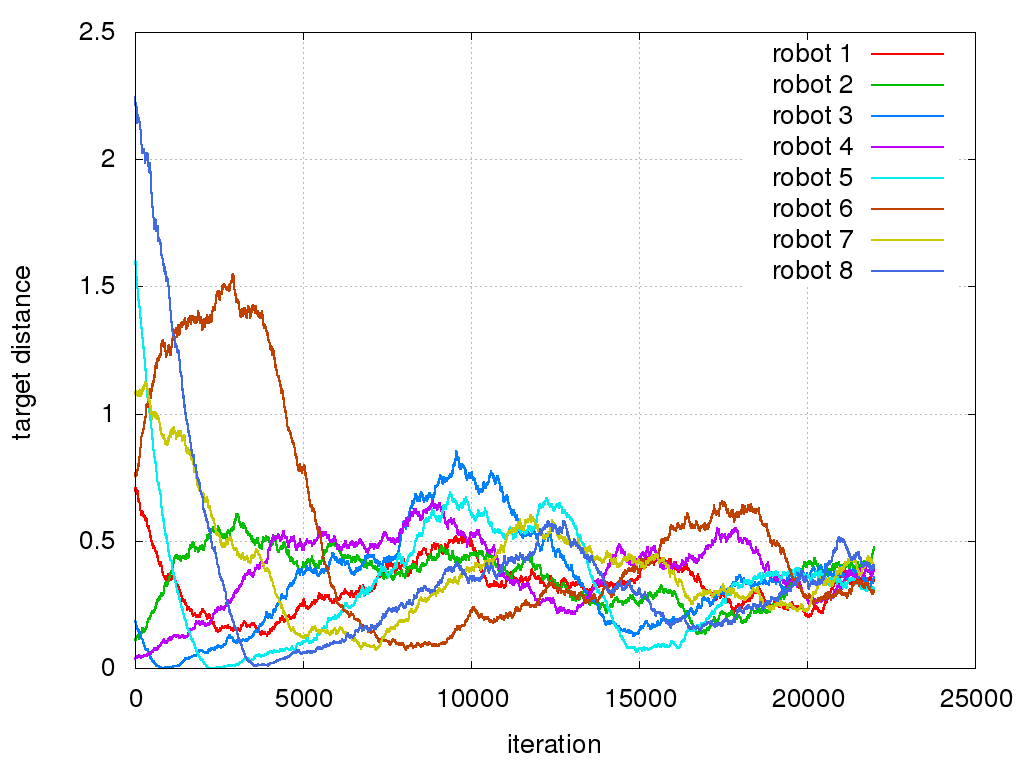
\includegraphics[scale=.4]{../../results_q_learning/nano_q_learning/result_04_02/robot_reward.png}
\caption{Vzdialenosť robotov od cieľa pre $\gamma = 0.7 p = 0.4$}
\label{img:nano_q_result_04_2_error}
\end{figure}


\begin{figure}[!htb]
\centering
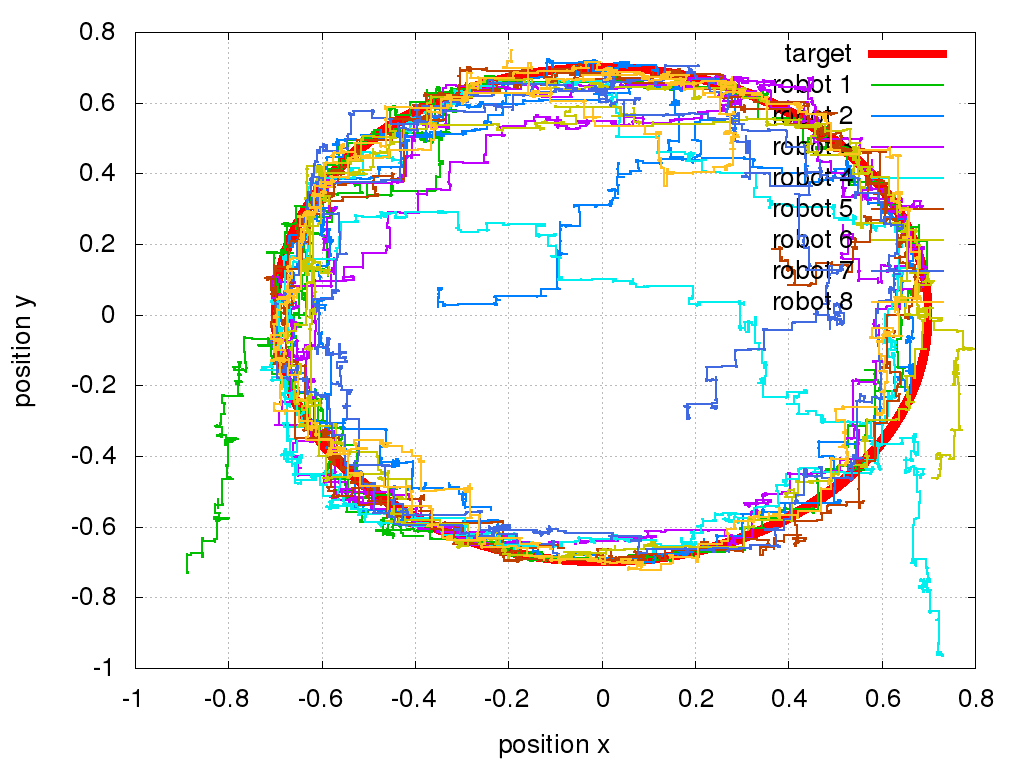
\includegraphics[scale=.4]{../../results_q_learning/nano_q_learning/result_04_03/robot_path.png}
\caption{Dráha robotov pre $\gamma = 0.9 p = 0.4$}
\label{img:nano_q_result_04_3_path}
\end{figure}

\begin{figure}[!htb]
\centering
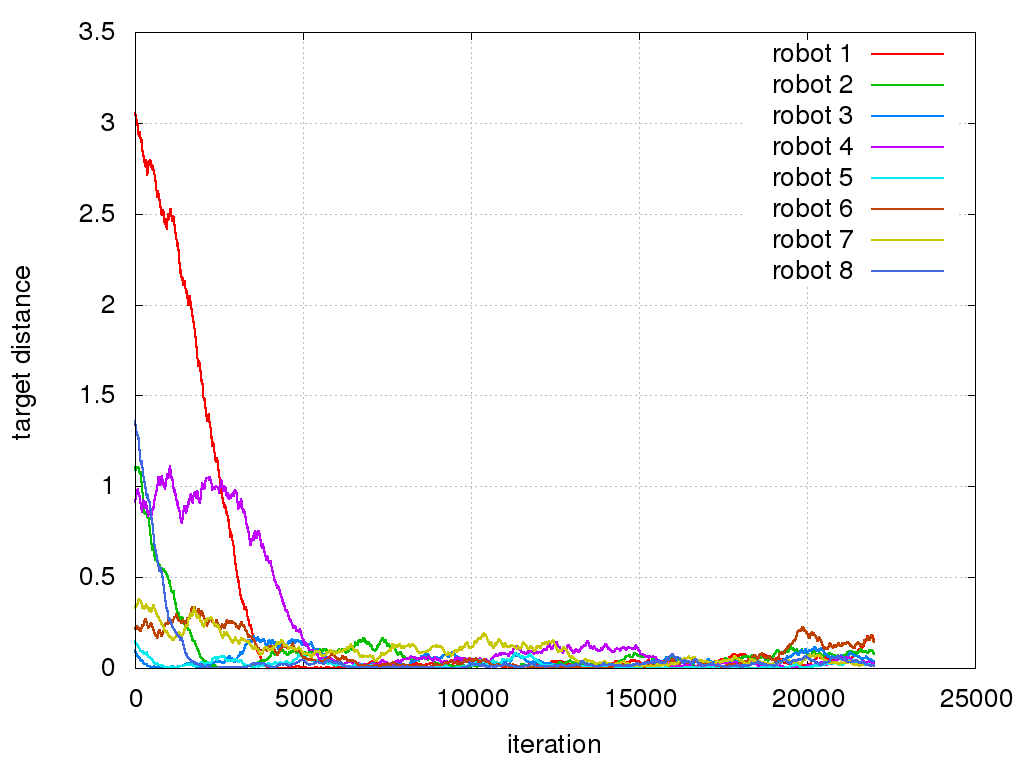
\includegraphics[scale=.4]{../../results_q_learning/nano_q_learning/result_04_03/robot_reward.png}
\caption{Vzdialenosť robotov od cieľa pre $\gamma = 0.9 p = 0.4$}
\label{img:nano_q_result_04_3_error}
\end{figure}

\begin{figure}[!htb]
\centering
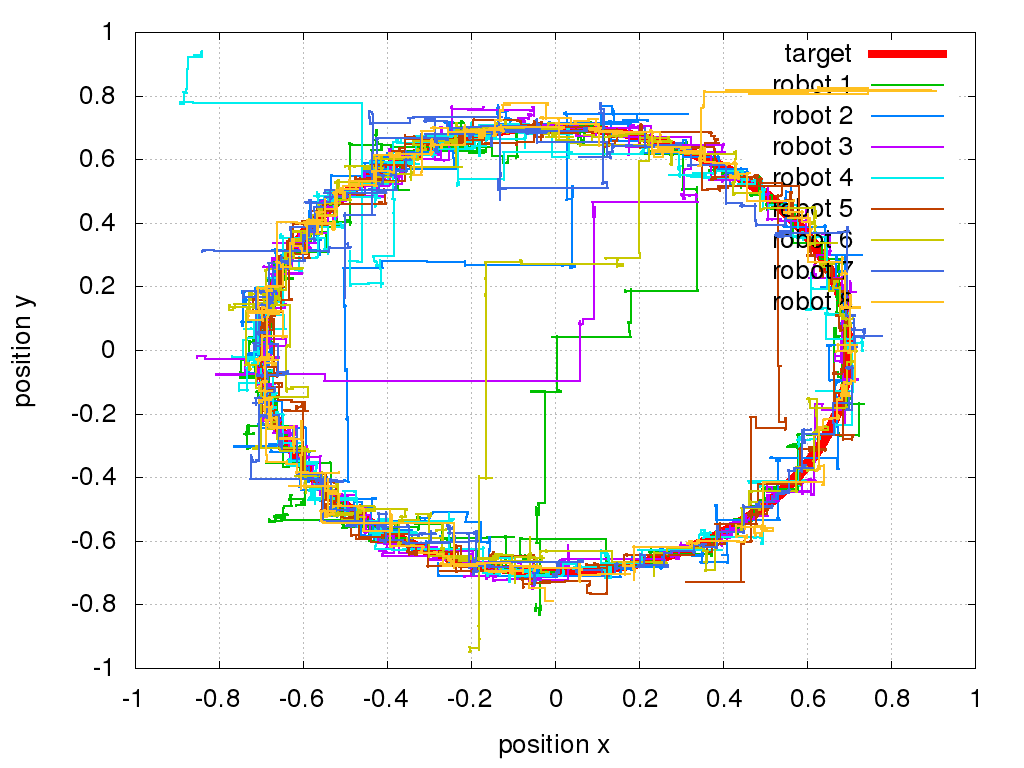
\includegraphics[scale=.4]{../../results_q_learning/nano_q_learning/result_04_04/robot_path.png}
\caption{Dráha robotov pre $\gamma = 0.98 p = 0.4$}
\label{img:nano_q_result_04_4_path}
\end{figure}

\begin{figure}[!htb]
\centering
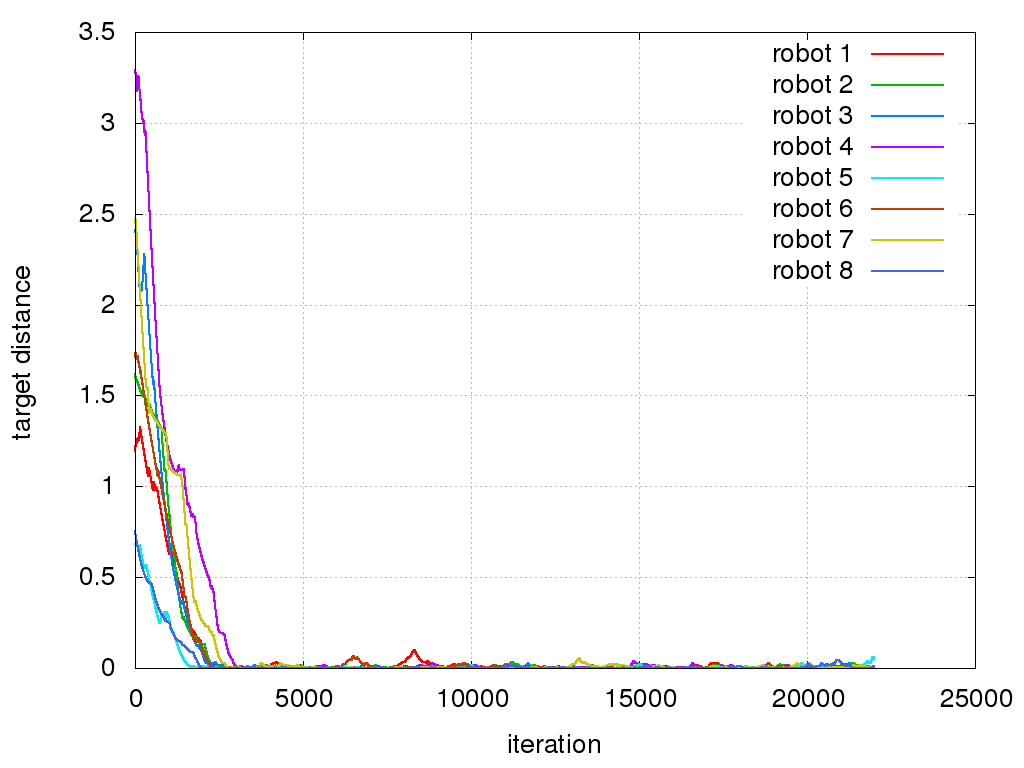
\includegraphics[scale=.4]{../../results_q_learning/nano_q_learning/result_04_04/robot_reward.png}
\caption{Vzdialenosť robotov od cieľa pre $\gamma = 0.98 p = 0.4$}
\label{img:nano_q_result_04_4_error}
\end{figure}

Z experimentov je zrejmé, že pre málo zašumené prostrednie nemá hodnota parametra
$\gamma$ veľký význam, obrázky :
\ref{img:nano_q_result_00_path}
\ref{img:nano_q_result_00_error},
\ref{img:nano_q_result_03_path}
\ref{img:nano_q_result_03_error}.

S postupným nárastom šumu však pri nevhodne zvolenej hodnote $\gamma$
roboti vykazujú veľkú chybu. Je preto tomu potrebné náležite zväčšovať
parameter $\gamma$, tento priebeh zlepšovania výsledku zvyšovaním parametra $\gamma$
je zrejmi z obrázkov :
\ref{img:nano_q_result_04_1_path}
\ref{img:nano_q_result_04_1_error},
\ref{img:nano_q_result_04_2_path}
\ref{img:nano_q_result_04_2_error},
\ref{img:nano_q_result_04_3_path}
\ref{img:nano_q_result_04_3_error},
\ref{img:nano_q_result_04_4_path}
\ref{img:nano_q_result_04_4_error}.

Algoritmus bol pomenovaný nanoQ a je pod licenciou GNU GPL dostupný na \cite{bib:nano_q_link}.
Je napísaný v jazyku C len s využitím pevnej rádovej čiarky. To umožňuje jeho implementáciu
aj do menej výkonných mikrokontrolérov, s jadrami napr. Cortex M0 alebo MSP430. Učenie
prebieha v reálnom čase a nevyžaduje veľký výpočtový výkon. Podobne, aj pamäťové nároky rastú
lineárne s počtom akcií. Pre veľký počet akcií je vždy možné použit aproximáciu, ktorá bude rozobratá
v neskorších častiach práce.

%\chapter{Q-larning algoritmus}

Q-learning algoritmus je definovaný pre časovo diskrétne systémy.
Agent ktorý prechádza stavový priestor vykonaním niektorej z vopred daných
akcií získava za tieto prechody odmeny. Cieľom algoritmu je ohodnotiť všetky akcie
v jednotlivých stavoch, tak aby bol dosiahnutý ustálený stav a v každom stave
bolo možno vybrať akciu prinášajúcu najväčšiu odmenu, v globálnom zmysle.


\section{Definícia algoritmu}

Daná je množina stavov $\mathbb{S}$ a akcií $\mathbb{A}$, kde
 $\mathbb{S} \in \mathbb{R}^{n_s}$ a $\mathbb{A} \in \mathbb{R}^{n_a}$, kde
$n_s$ a  $n_a$ sú počty prvkov stavového vektora a vektora akcií.

Existuje prechodová funkcia
\begin{align}
        s(n+1) = \lambda(s(n), a(n))
\end{align}

zo stavu $s(n) \in \mathbb{S}$ použitím akcie $a(n) \in \mathbb{A}$, táto funkcia je ale algoritmu neznáma.

Ďalej je daná odmeňovacia funkcia $R(s(n),a(n))$, ktorá vyjadruje okamžité ohodnotenie konania
agenta v $s(n)$ a $a(n)$. V reálnych aplikáciach táto funkcia nadobúda takmer v každom
$s(n)$ a $a(n)$ hodnotu $0$. Pre správnu funkciu algoritmu, musí byť aspoň jedna hodnota
nenulová - napr. ohodnotenie dosiahnutia cieľového stavu (samotná existencia cieľového
stavu však pre algoritmus nie je potrebná).

Funkcia ohodnotení je definovaná ako

\begin{equation}
Q_{n}(s(n),a(n)) = R(s(n),a(n)) + \gamma \max_{a(n-1) \in \mathbb{A}} Q_{n-1}(s(n-1), a(n-1))
\label{eq:q_learning}
\end{equation}

\begin{itemize}
 \item $R(s(n),a(n))$ je odmeňovacia funkcia
 \item $Q_{n-1}(s(n-1),a(n-1))$ je funkcia ohodnotení v stave $s(n-1)$ pre akciu $a(n-1)$
 \item $\gamma$ je odmeňovacia konštanta a platí $\gamma \in (0, 1)$.
\end{itemize}

Funkcia $\ref{eq:q_learning}$ definuje ohodnotenie akcií vo všetkých stavoch t.j.
agent ktorý sa dostal do stavu $s(n)$ vykonaním akcie $a(n)$ zo stavu
$s(n-1)$ získal odmenu $R(s(n),a(n))$ a zlomok najväčšieho možného ohodnotenia ktoré
mohol získať dostaním sa do stavu $s(n-1)$, situáciu ilustruje obrázok \ref{img:q_learning}.


\begin{figure}[!htb]
\center
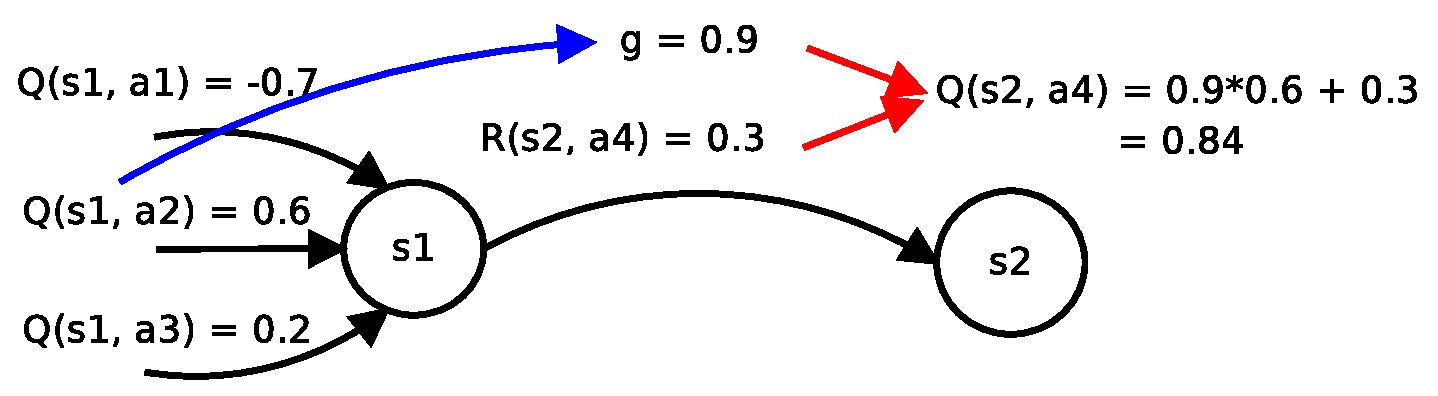
\includegraphics[scale=.6]{../diagrams/q_learning_detail.eps}
\caption{Ilustrácia funkcie ohodnotení, pre $\gamma = 0.9$}
\label{img:q_learning}
\end{figure}

Nasledujúce obrázky ilustrujú beh algoritmu pre systém so 6 stavmi pre $\gamma = 0.8$.
Na začiatku nie sú známe ani samotné prechody medzi stavmi (Obr. $\ref{img:q_learning_1}$), bol definovaný
1 cieľový stav $S5$, agent začína v stave $S0$ (môže však v ľubovolnom inom).
Ďalej sa pre jednoduchosť predpokladá že

\begin{equation}
R(s(n), a(n)) =
\left\{
	\begin{array}{ll}
		1  & ak \ s(n) = $S5$ \\
    -0.5  & ak \ s(n) = $S4$ \ \wedge \ $a(n) = Ay$  \\
		0 & inak
	\end{array}
\right.
\label{eq:r_func_simple}
\end{equation}

t.j. odmeňovacia funkcia nadobúda hodnotu $1$ len ak sa agent dostal do stavu
$S5$ a pre ilustráciu je definovaná aj jedna záporná odmena pri prechode z $S4$ do
$S3$ akciou $Ay$.

\begin{figure}[!htb]
\center
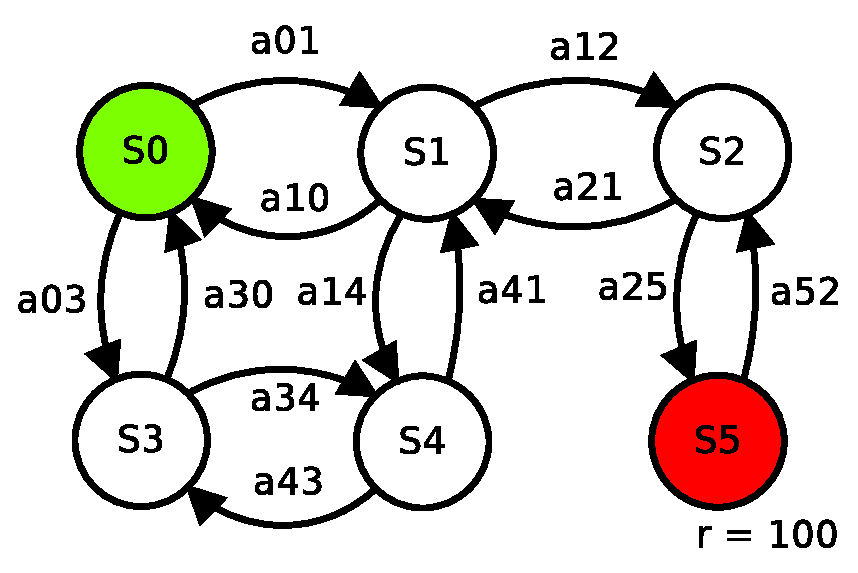
\includegraphics[scale=.6]{../diagrams/q_learning_table_01.eps}
\caption{Inicializácia}
\label{img:q_learning_1}
\end{figure}

Agent v každom stave náhodne vyberá akcie (na výbere nezáleží, dôležité je aby
každá akcia mala nenulovú pravdepodobnoť výberu, a rovnako bola nenulová
prevdepodobnosť dosiahnutia ľubovolného stavu). Obrázky Obr. \ref{img:q_learning_2}
a Obr. \ref{img:q_learning_3} ilustrujú jednu z možných ciest.


\begin{figure}[!htb]
\center
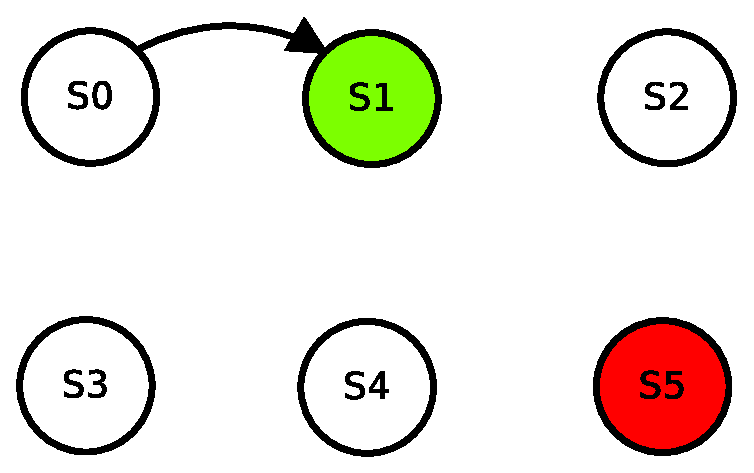
\includegraphics[scale=.6]{../diagrams/q_learning_table_02.eps}
\caption{Prechod do stavu S1}
\label{img:q_learning_2}
\end{figure}

\begin{figure}[!htb]
\center
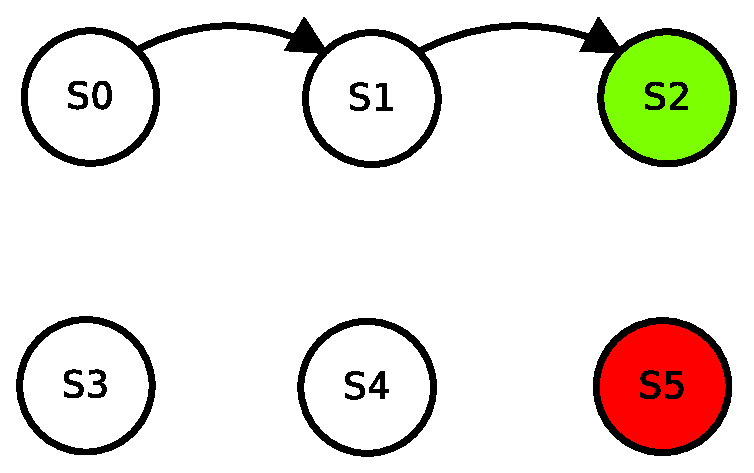
\includegraphics[scale=.6]{../diagrams/q_learning_table_03.eps}
\caption{Prechod do stavu S2}
\label{img:q_learning_3}
\end{figure}

Po dosiahnutí cieľového stavu Obr. \ref{img:q_learning_4} je na základe \ref{eq:r_func_simple}
možné spočítať podľa \ref{eq:q_learning} ohodnotenia doteraz vykonaných akcií -
agent získal nenulovú odmenu $R(s_5, a_x) = 1$ (kde $a_x$ značí ľubovolnú akciu),
ktorú rekurentne spočíta pre všetky doteraz vykonané akcie.

Pre zjednodušenú variantu \ref{eq:q_learning} by bolo možné pamätať si len jeden
predošlý stav a nepostupovať v ohodnocovaní rekuretne. V praktickej aplikácií
je potrebné obmedziť hĺbku rekurzie, a pamätať si len posledných $P$ stavov a vnich
urobených rozhodnutiach. V tomto jedńoduchom príklade však nie sú nutné tieto obmedzenia, je teda
možné pamätať si celú cestu.

\begin{figure}[!htb]
\center
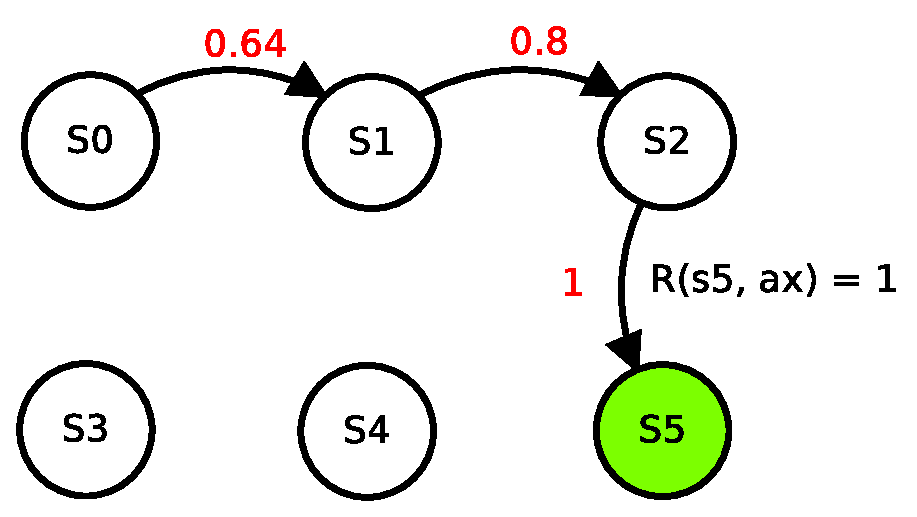
\includegraphics[scale=.6]{../diagrams/q_learning_table_04.eps}
\caption{Prechod do stavu S3}
\label{img:q_learning_4}
\end{figure}

Agent môže pokračovať v ceste ďalej, napr. späť \ref{img:q_learning_5} a pribežne
počítať ohodnotenia. Prechod z $s_5$ do $s_2$ je ohodnotený ako $0.8$ - vybralo sa najlepšie
možné ohodnotenie ako sa dostať do $s_5$ ($1$) násobené $\gamma$, $R(s_2, a_x) = 0$
(podľa \ref{eq:r_func_simple}).


\begin{figure}[!htb]
\center
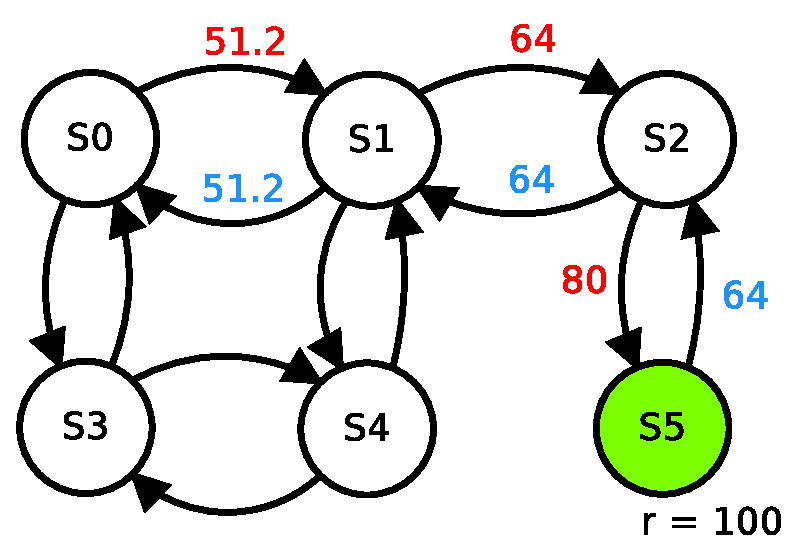
\includegraphics[scale=.6]{../diagrams/q_learning_table_05.eps}
\caption{Ďalšie prechody agenta}
\label{img:q_learning_5}
\end{figure}

Po prejdení celého grafu, kedy agent vykonal všetky možné akcie dosiahne
funkcia $Q(s(n), a(n))$ konečný, ustálený stav Obr. \ref{img:q_learning_6}, teda

\begin{equation}
\forall s(n),\ \forall a(n),\forall \epsilon > 0 \  \exists Q_{n} : \mid Q_{n}(s(n), a(n)) - Q_{n-1}(s(n), a(n)) \mid < \epsilon
\label{eq:q_learning_finish}
\end{equation}

hodnoty Q-funkcie sa teda pri pevne danom $R(s(n), a(n))$ už nemenia.


\begin{figure}[!htb]
\center
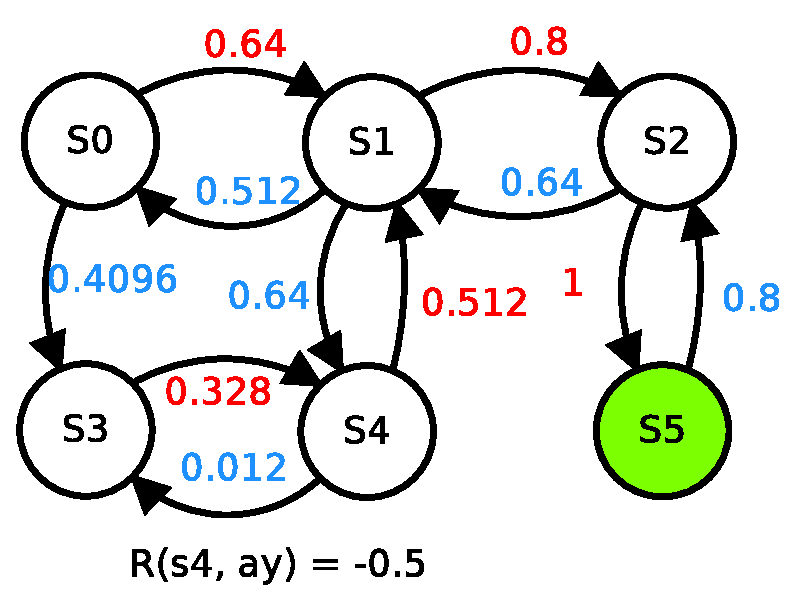
\includegraphics[scale=.6]{../diagrams/q_learning_table_06.eps}
\caption{Konečný stav}
\label{img:q_learning_6}
\end{figure}


\section{Výber akcie}

Pre nájdenie konečných hodnôt funkcie ohodnotení podľa \ref{eq:q_learning_finish}
stačí aby každý prechod mal nenulovú pravdepodobnosť vykonania. Pre ďalšie vyšetrovanie
konania agenta ja daná pravdepodobnosť výberu akcie  ako

\begin{equation}
P(s(n), a(s)) = \frac{e^{kQ(s(n), a(s))}}{ \sum\limits_{i=1}^{C_a}{e^{kQ(s(n), a(i))}} }
\label{eq:action_selection}
\end{equation}

kde \\
$s$ je zvolená akcia \\
$C_a$ je počet akcií \\
$k$ je konštanta a platí $k \geq 0$

agent ktorý vyberá všetky akcie s rovnakou pravdepodobnosťou má teda $k = 0$.
Pre vysoké hodnoty $k$ : $\lim_{k\to\infty}$ bude agent vyberať len najlepšie
dostupné akcie. Pre učenie agenta je teda vhodné zvoliť malé $k$.

Je možné definovať ľubovolné iné možnosti výberu akcie, napr. uprednostňovať menej
často vykonané akcie, prípadne podľa zmeny
$\mid Q_{n}(s(n), a(n)) - Q_{n-1}(s(n), a(n)) \mid$ uprednostňovať prechody s veľkou hodnotou zmeny.


\section{Problémy výpočtu $Q(s, a)$}

Algoritmus je definovaný pre diskrétnu množinu stavov. Ďalej sa predpokladá, že
$s(n) \in \langle -1, 1 \rangle$ a podobne $a(n) \in \langle -1, 1 \rangle$

 Pre počty prvkov
stavového vektora a vektora akcií ($n_s$, $n_a$) je možné definovať
delenie ich hodnôt na diskrétny počet $d_s$ a $d_a$, potom je možné vyjadriť celkový počet
hodnôt $Q(s(n), a(n))$ ako

\begin{equation}
C = {d_s}^{n_s} {d_a}^{n_a}
\label{eq:q_size}
\end{equation}

Samotný počet hodnôt ktoré treba spočítať teda exponenciálne narastná s rastom
počtu prvkov stavového a vektora akcií.

Pre úlohy kde do systému vstupuje mnoho nezávislých vstupov sa stáva implentácia Q(s(n), a(n))
problémom najmä z dôvodov :

\begin{itemize}
\item veľké pamäťové nároky
\item o nenavštívených prechodoch nevie agent povedať nič
\end{itemize}

Vhodným riešením sa ukazuje aproximácia Q-funkcie.
Nech je aproximovaná funkcia označená $Q_n'(s(n), a(n))$ a presné riešenie ako $Q_n(s(n), a(n))$.

Dané sú postuláty o tejto aproximácií
\begin{theorem}{Neobmedzená prenosť aproximácie : }
\label{post:01}
Pre všetky stavy $s(n)$ a akcie $a(n)$ musí platiť
$\mid Q_n(s(n), a(n)) - Q_n'(s(n), a(n)) \mid < \epsilon $. Kde $\epsilon > 0$ a
určuje kvalitu aproximácie. Zlepšením vlastností $Q_n'(s(n), a(n))$ je možné
ľubovolne zmenšovať  $\epsilon$.
\end{theorem}

\begin{theorem}{Lokálna zmena : }
\label{post:02}
Lokálna zmena hodnoty $\delta = \mid Q_n'(s(n), a(n)) - Q_{n-1}'(s(n), a(n)) \mid$ neovplyvní hodnotu funkcie v
inom bode o viac ako $\forall \ s(n') \ \forall a(n'),\ n \neq n' : \delta < \kappa$.
Zmenšovaním hdonoty $\kappa$ sa funkcia stáva menej závislá na okolí bodu $[s(n), a(n)]$.
\end{theorem}

Funkciu $Q(s(n), a(n))$ je možné aproximovať niekoľkými spôsobmi.
Tie najbežnejšie sú

\begin{itemize}
\item tabuľka
\item neurónová sieť
  \begin{itemize}
    \item dopredná neurónová sieť
    \item kohonenova mapa
    \item neurónová sieť bázickych funkcií
  \end{itemize}
\end{itemize}

\section{Tabuľka}

Priamočíarým prístupm je ukladať hodnoty $Q(s(n), a(n))$ do tabuľky. Pre
diskrétnu a konečnú množinu akcií možno tabuľku rozdeliť na viac častí,
čím sa urýchli vyhľadávanie. Počet stavov v reálnych aplikáciach však môže byť
vysoký (vo všeobecnosti tvoria stavy spojitú množinu).

Stav agenta aj vykonaná akcia sú obvykle vektory normované do $\langle -1, 1 \rangle$,
pre implementáciu tabuľky je nutné ich prepočítať na celočíselné indexy

\begin{align}
  I_s(n) = \lceil \sum\limits_{i=1}^{n_s} {\left( d_s\frac{s_i(n) + 1}{2} \right)^i \rceil}  \\
  I_a(n) = \lceil \sum\limits_{i=1}^{n_a} {\left( d_a\frac{a_i(n) + 1}{2} \right)^i \rceil}
\end{align}

kde \\
$I_s(n)$ je index stavu \\
$I_a(n)$ je index akcie \\
$s_i(n)$ je i-ty prvok vektora stavu $s(n)$ \\
$a_i(n)$ je i-ty prvok vektora akcií $a(n)$ \\

Pre diskrétny počet stavov a akcií je možné definovať tabuľkovú interpretáciu ako
$Q^t(I_s(n), I_a(n))$.
Pre $\lim_{d_s\to\infty}$ a $\lim_{d_a\to\infty}$ je možné považovať tabuľku za presné riešenie
pretože spĺňa postuláty \ref{post:01} aj \ref{post:02}.

\section{Dopredná neurónová sieť}

Pre aproximáciu funkcie ohdnotení je možné použiť dobrednú neurónovú sieť ako
univerzálny aproximátor. Podľa Kolmogorovho teorému je možné neurónovú sieť
takto použiť \cite{bib:kolomongorov_01}, \cite{bib:kolomongorov_02} a \cite{bib:kolomongorov_03}.
Samotný teorém však nerieši problém učenia takejto siete. Na učenie siete
existuje niekoľko algoritmov, medzi najčastejšie patria
\cite{bib:backpropagation_00}, \cite{bib:backpropagation_01}, \cite{bib:backpropagation_02} :

\begin{enumerate}
 \item Backpropagation
 \item Genetické algoritmy
 \item Simulované žíhanie
\end{enumerate}

Najpoužívanejší Backpropagation má množstvo problémov, najmä postupný pokles gradientu
v hlbokých neurónových sieťach. Kedy sú vnorené vrstvy prakticky neučené. Ďalší závažný problém
je uviaznutie v lokálnom minime, čo sa autory snažia vyriešiť zavedným zotrvačnosti
do zmeny váh siete. Istým nádejným východiskom sa zdá byť simulované žíhanie \cite{bib:annealing_01}.
Pre problém Q-learning algoritmu je však potrebný prístup ktorý postupne zlepšuje riešenie,
a to je jedine niektorá z gradientových metód.

Samotná dopredná sieť je tvorená niekoľkými prepojenými vrstvami neurónov \ref{img:ffnn}.
Pre popis vrstvy je však vhodné použiť maticový zápis, nakoľko prenos neurónu má
obvykle vo vrstve rovnakú aktivačnú funkciu.

\begin{figure}[!htb]
\center
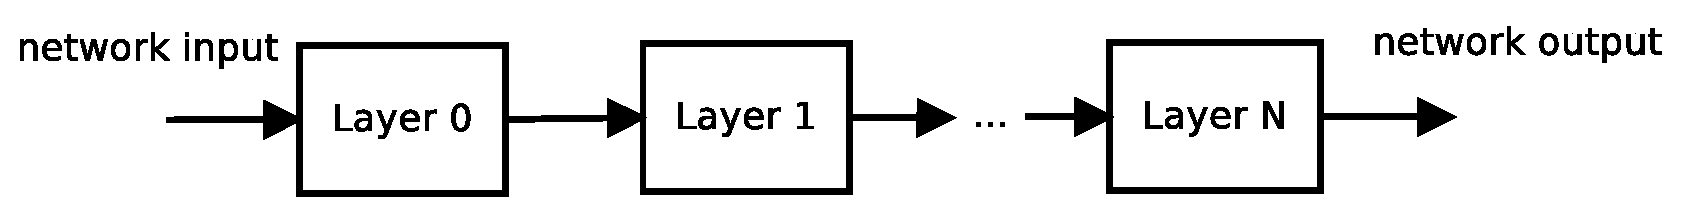
\includegraphics[scale=.6]{../diagrams/neural_layers.eps}
\caption{Dopredná neuronová siet}
\label{img:ffnn}
\end{figure}

Správanie sa jednej vrstvy je možné popísať ako funkciu vstupného vektora,
ktorej výstupom je tiež vektor (počty prvkov týchto vektorov však môžu byť rôzne,
vždy však konečné).
Je daný vstupný vektor

\begin{align}
I(n) = (s(n), a(n))
\label{eq:nn_input_vector}
\end{align}

výstupná hodnota neurónovej siete ako $y_{nn}(n)$ a požadovaná hodnota ako $y_{r}(n)$.

Ďalej je definovaná chyba ako

\begin{align}
e(n) = y_{r}(n) - y_{nn}(n)
\label{eq:nn_error}
\end{align}

Vrstva $l$ doprednej siete je definovaná ako
\begin{align}
y^l(n) &= f^l\left(W^l(n)I^l(n)\right) \nonumber \\
 &= f^l\left(
 \begin{pmatrix}
  w^l_{1,1}(n) & w^l_{1,2}(n) & \cdots & w^l_{1,n'}(n) \\
  w^l_{2,1}(n) & w^l_{2,2}(n) & \cdots & w^l_{2,n'}(n) \\
  \vdots  & \vdots  & \ddots & \vdots  \\
  w^l_{m',1}(n)  & w^l_{m',2}(n)  & \cdots & w^l_{m',n'}(n)
 \end{pmatrix}
 \begin{pmatrix}
  i^l_{1,1}(n) & i^l_{1,2}(n) & \cdots & i^l_{1,n'}(n) \\
 \end{pmatrix}
 \right)
 \label{eq:nn_layer}
\end{align}

kde \\
$n'$ je počet prvkov vstupného vektora \\
$m'$ je počet prvkov výstupného vektora \\
$f(X)$ je aktivačná funkcia \\
$W^l(n)$ je matica váh.

Najčastejšie používané aktivačné funkcie sú sigmoida, hyberbolický tangens , lineárna,
usmerňovač a skoková funkcia. Ich predpisy sú

\begin{align}
y_1(x) &= \frac{1}{1+e^{-x}} \\
y_2(x) &= \frac{e^{x} - e^{-x}}{e^{x} + e^{-x}} \\
y_3(x) &= x \\
y_3(x) &= \left\{
	\begin{array}{ll}
		x  & ak \ x > 0 \\
		0 & inak
	\end{array}
\right. \\
y_4(x) &= \left\{
	\begin{array}{ll}
		1  & ak \ x > 0 \\
		-1 & inak
	\end{array}
\right.
\label{eq:nn_transfer_function}
\end{align}

Ich priebehy sú znázornené na obrázku \ref{img:nn_functions}.

\begin{figure}[!htb]
\center
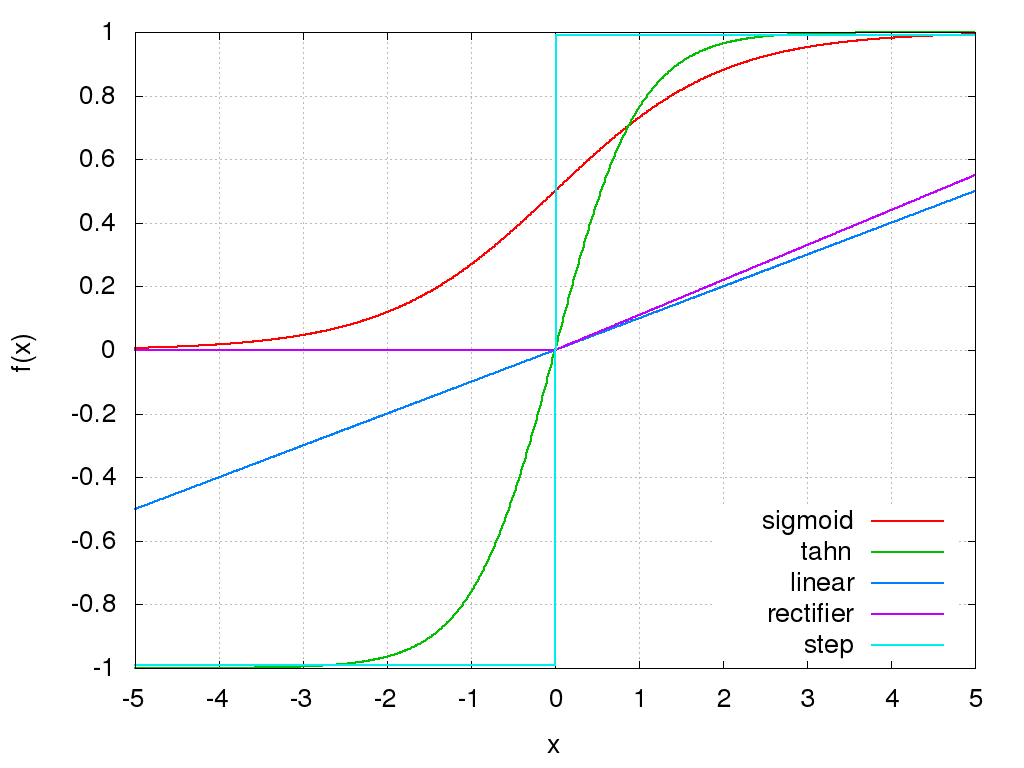
\includegraphics[scale=.4]{../pictures/nn_functions.png}
\caption{Grafické znázornenie priebehov aktivačných funkcií}
\label{img:nn_functions}
\end{figure}

Zoradením niekoľkých vrstiev za sebou, tak že výstup predošlej je vstupom do aktuálnej
vrstvy je možné získať doprednú neurónovu sieť. Takáto sieť je vhodná na riešenie klasifikačných
aj aproximačných problémov.

Dopredná sieť je známa nelokálnosťou učenia : pri trénovaní na podmnožinu množiny
požadovaných výstupov sa mení hodnota aj mimo túto podnmožinu. Sieť teda veľmi
problematicky spĺňa postutlát \ref{post:02}. Dobre však spĺňa postulát \ref{post:01},
vhodnou voľbou počtu vrstiev a počtu neurónov je možné dosiahnúť ľubovolnú
presnosť aproximácie.

\section{Kohonenová neurónová sieť}

Kohonenova neurónová sieť je inšpirovaná rovinnými štruktúrami v mozgovej kôre,
kde výrazne dominujú prepojenia v rámci vrstvy a prepojení medzi vrstvami je
podstatne menej \ref{img:cortical_column}. Napriek týmto rovinatým štruktúram,
mozog bežne spracúva mnohodimenzionálne problémy - vstupm sú podnety s miliónov
receptorov.

\begin{figure}[]
\center
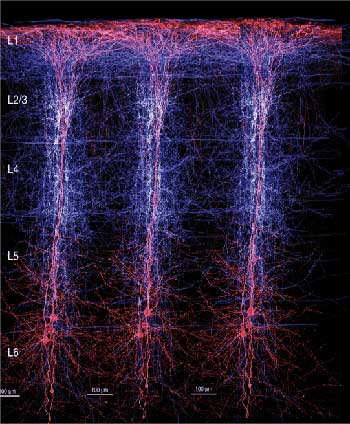
\includegraphics[scale=.4]{../pictures/cortical_column.jpg}
\caption{Neokortexový stĺpec}
\label{img:cortical_column}
\end{figure}

Pôvodný návrh Kohonenovej siete neriešil aproximáciu funkcie, ale klasifikáciu
vstupov do zhlukov. Pričom podobné vstupy patria do rovnakého zhluku. Počet zhlukov
je voliteľný a je rovný počtu použitých neurónov. Takáto sieť sa vie učiť bez
definovania chyby, t.j. nie je potrebné stanoviť do ktorého zhluku dáta patria. Samotné
zhluky sa utvárajú postupne, tak ako sú do siete predkladané dáta.

Každému zhluku je však možné priradiť požadovanú výstupnú hodnotu. Sieť tak môže
pracovať podobne ako tabuľka - vstupné dáta priradí do najbližšieho zhluku a výstupom
je hodnota prisluchújalúca k tomuto zhluku. V tomto prípda už treba stanoviť chybu,
ako rozdiel požadovanej hodnoty a skutočnej hodnoty výstupu siete.
Algoritmus má niekoľko krokov :
\\
Najpr sa spočítajú vzdialenosti od vstupného vektora

\begin{align}
d_j(n) = \sum\limits_{i=1}^{N}{(I_i(n) - w_{ji}(n))^2}
\label{eq:knn_distance}
\end{align}

kde $w(n) \in \mathbb{R}$ je matica váh, na začiatku sa volí náhodná, tak
aby rovnomerne pokrila stavový priestor vstupných veličín (Obvykle sa používa rovnomerné
rozdelenie. Štatistickou analýzou vstupných dát je ale možné určiť iné, vhodnejšie
a urýchliť tak konvergenciu hodnôt váh).

Víťazný neurón $v$ je definovaný ako

\begin{align}
v : \forall j : d_v(n) \leq d_j(n)
\label{eq:knn_winning}
\end{align}

je to neurón ktorý má najmenšiu vzdialenosť od predloženého vstupu.

A pre každý neurón existuje priradená výstupná hodnota $y_j(n) \in \mathbb{R}$, výstupom
siete je teda hodnota priradená výťaznému neurónu $y_{nn}(n) = y_v(n)$.


Učenie siete prebieha v dvoch krokoch

{1) \bf zmena váh $w(n)$ } zmenia sa váhy výťazného neurónu, pretože najlepšie
zodpovedajú požadovaným váham tak že sa priblížia hodnote vstupného vektora

\begin{align}
w_{ji}(n+1) = (1-\eta_1(j))w_{ji}(n) + \eta_1 I_i(n)
\label{eq:knn_w_update}
\end{align}

kde $\eta_1(j) \in (0, 1)$ je krok učenia a závisí od polohy neurónu v sieti.
V najjednoduhšom prípade

\begin{equation}
\eta_1(j) =
\left\{
	\begin{array}{ll}
		\eta  & ak \ j = v \\
		0 & inak
	\end{array}
\right.
\label{eq:knn_func_simple1}
\end{equation}

k zmene váh teda dôjde len pri víťaznom neuróne.
Ďalší často používaný tvar funkcie postupne zmenšuje hodnotu $\eta_1(j)$ podľa
$d_j(n)$ a to ako

\begin{align}
\eta_1(j, n) = \eta e^{-kd_j(n)}
\label{eq:knn_func_simple2}
\end{align}

kde $k \in (0, \infty )$. Krok učenia $\eta_1(j, n)$ je teda premenný a záleží
aj od predloženého vzoru podľa $n$.

Po dostatočnom počte iterácií sa hodnoty váh ustália na hodnotách tak aby rozdelili
množinu vstupných vektorov na lokálne oblasti. Tento stav je znázornený na \ref{img:knn_learning_result}.
Vstupný proces generoval 8 zhlukov dát ktoré sieť klasifikovala použitím 16 neurónov.
Každému neurónu je možne priradiť požadovanú hodnotu výstupu.

{2) \bf upraví sa výstupná hodnota $y_v(n)$}

\begin{align}
y_v(n+1) = y_v(n) + \eta_2 e(n)
\label{eq:knn_y_update}
\end{align}

kde $e(n)$ je chyba podľa \ref{eq:nn_error}.
Takáto Kohonenová sieť má veľmi dobré predpoklady na aprixmáciu funkcie,
ktorá nadobúda málo hodnôt, predkladaním vzorov z blízkosti
jedného zhluku (dáta majú malú vzdialenosť v zmysle \ref{eq:knn_distance} )
sa dá očakávať zmena parametrov len jedného neurónu. Sieť teda dobre spĺňa predpoklady
\ref{post:01},  \ref{post:02}. Počet neurónov však musí narásť do nekonečna.

Je vhodné poznamenať, že výstupná hodnota nemusí byť len číselná hodnota, ale aj funkcia, ktorej vstupom je opäť
$I_i(n)$. Výber výťazného neurónu tak funguje ako výber vhodnej funkcie - prepínač.

\begin{figure}[]
\center
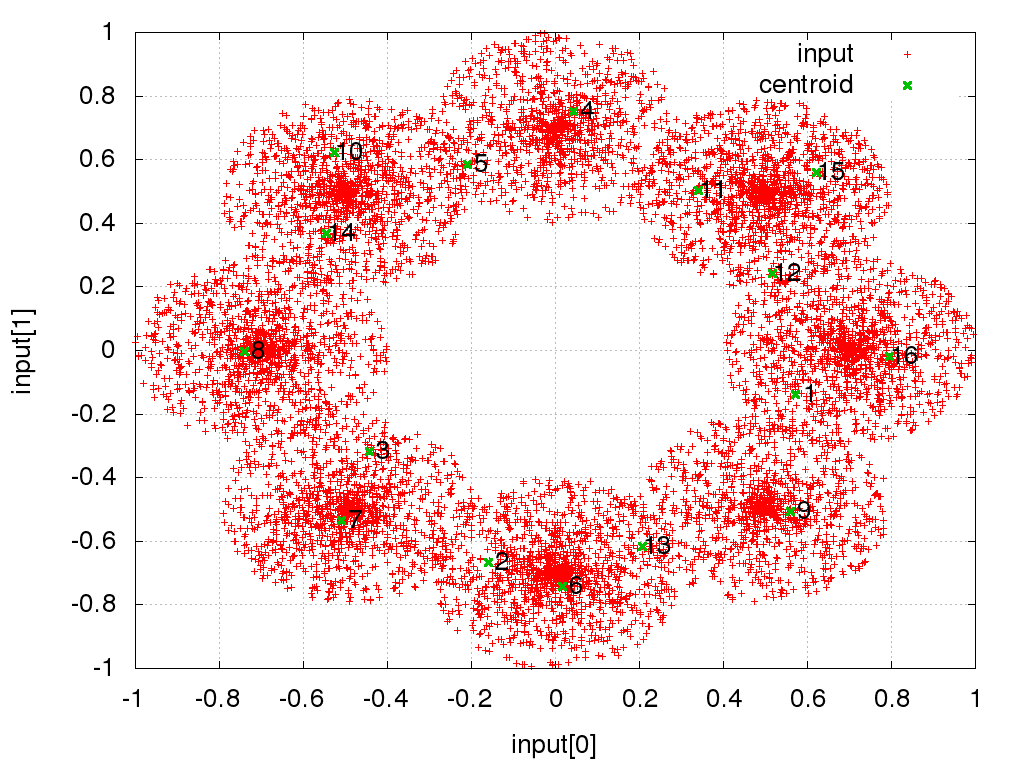
\includegraphics[scale=.4]{../pictures/knn_learing_result.png}
\caption{Znázornenie váhových parametrov w pre dvojrozmerný priestor}
\label{img:knn_learning_result}
\end{figure}

.

\section{Neurónová sieť bázickych funkcií}

Samotný prenos neurónu nemusí byť obmedzený len na množinu funkcií z \ref{eq:nn_transfer_function}.
Vhodnú funkciu je možné zmenou parametrov upraviť do tvaru, aby na zvolený
vstup $I_0(n)$ dosahovala požadovanú hodnotu a postupným zväčšovaním
vzdialenosti $\mid I_0(n) - I_i(n) \mid$ klesala jej hodnota k nule.

Najjednoduhším príkladom takýchto funkcií  je


\begin{equation}
f_j(X(n)) =
\left\{
	\begin{array}{ll}
		k_j  & ak \ X(n) = X_0 \\
		0 & inak
	\end{array}
\right.
\label{eq:bfnn_simple}
\end{equation}

kde $k_j$ je hodnota požadovaná v bode $X_0$. Výstupom siete potom je

\begin{align}
y(X) = \sum\limits_{j=1} f_j(X(n))
\label{eq:bfnn_simple_res}
\end{align}

Z charakteru Q-learning algoritmu majú hodnoty $Q(s(n),a(n))$ charakter aj
postupne klesajúcich hodnôt. Je teda potrebné vybrať iné funkcie.

Nasledujú preto definície funkcií s ktorými boli urobené experimenty.

Dané sú bázické funkcie $f_j^x(\boldmath{s(n), a(n)})$, kde $x$ je typ bázickej funkcie.
Požadovaná hodnota $Q^x(s(n), a(n))$ je potom lineárnou kombináciou týchto funkcií typu $x$.

Z charakteru Q-learning algoritmu \ref{eq:q_learning} je možné určiť požiadavky na
tieto funkcie :

\begin{enumerate}
\item predpis \ref{eq:q_learning} je tvorený klesajúcou exponenciálou - podobný charakter by mala mať aj bázická funkcia
\item existencia jedného globálneho maxima a zmenou parametrov určovať polohu tohto bodu
\item možnosť ľubovolne meniť strmosť funkcie v okolí maxima
\item funkcia by mala byť zhora aj z dola ohraničená
\end{enumerate}

Cieľom je mať možnosť nezávisle nastaviť maximá funkcií do oblastí, ktoré zodpovedajú
nenulovím hodnotám $R(s(n), a(n))$ - bod 2. Ak ohodnotenie spĺňa podmienku najlepšej
možnej akcie v danom stave, dá sa očakávať že bude mať menšiu strmosť, naopak, ak funkcia
popisuje bod kde $R(s(n), a(n))$ dosahuje malé hodnoty (obvykle záporné), bude požadovaná
vysoká strmosť tejto funkcie - obe požiadavky sú zhrnuté v bode 3. Bod 4 umožňuje rozumne
ohraničiť rozsah funkcie.

Niektoré tvary bázických funkcií
\begin{align}
    f_j^1(\boldmath{s(n), a(n)}) &= e^{ -\sum\limits_{i=1}^{n_s}{\beta_{aji}(n)(s_i(n) - \alpha_{aji}(n))^2} }  \\
    f_j^2(\boldmath{s(n), a(n)}) &= \frac{1}{1 + \sum\limits_{i=1}^{n_s}{\beta_{aji}(n)(s_i(n) - \alpha_{aji}(n))^2}}  \\
    f_j^3(\boldmath{s(n), a(n)}) &= e^{ -\sum\limits_{i=1}^{n_s}{\beta_{aji}(n)\mid s_i(n) - \alpha_{aji}(n) \mid} }
\end{align}

kde \\
$\alpha_{aji}(n) \in \langle -1, 1 \rangle$ určuje polohu maxima funkcie \\
$\beta_{aji}(n) \in (0, \infty)$ určuje strmosť funkcie.

Ich priebeh pre prvé dve je na \ref{img:basis_funcions}.

\begin{figure}[]
\center
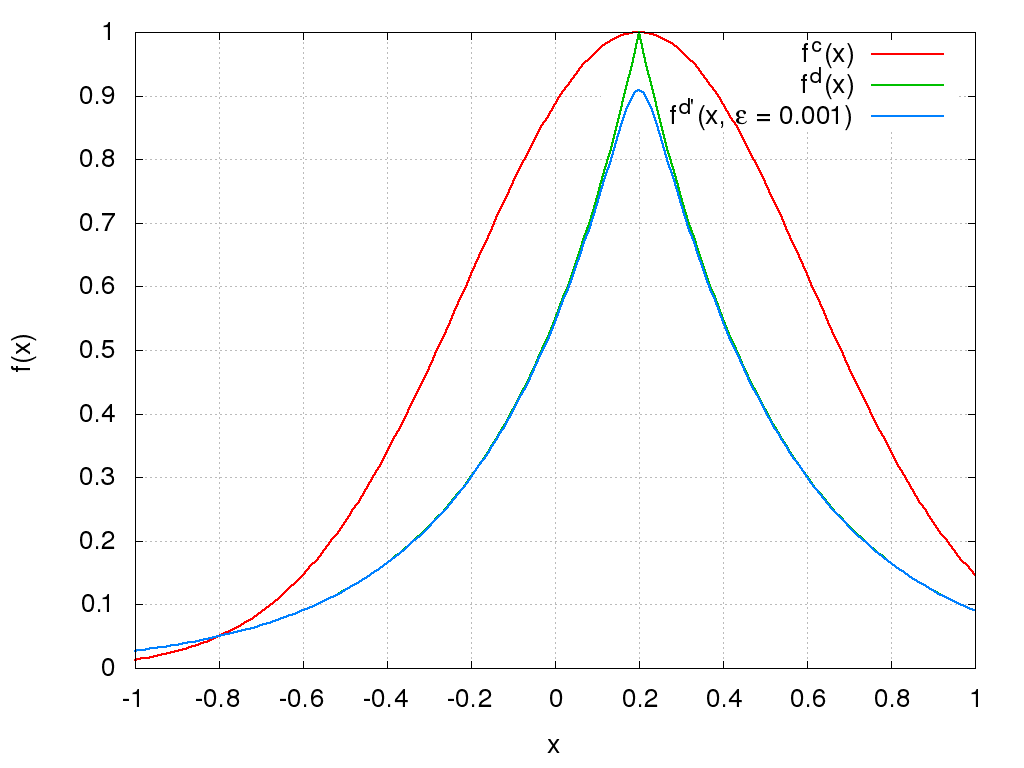
\includegraphics[scale=.4]{../pictures/gaussian_1D.png}
\caption{Znázornenie priebehov bázických fukcií}
\label{img:basis_funcions}
\end{figure}

Pre symetrické prechody medzi stavmi ich možno zjednodušiť na

\begin{align}
f_j^1(\boldmath{s(n), a(n)}) &= e^{ -\beta_{aj} \sum\limits_{i=1}^{n_s}{(s_i(n) - \alpha_{aji})^2} }  \\
f_j^2(\boldmath{s(n), a(n)}) &= \frac{1}{1 + {\beta_{aj} \sum\limits_{i=1}^{n_s}(s_i(n) - \alpha_{aji})^2}}  \\
f_j^3(\boldmath{(n)s, a(n)}) &= e^{ -\beta_{aj} \sum\limits_{i=1}^{n_s}{\mid s_i(n) - \alpha_{aji}(n) \mid} }
\label{eq:basis_functions}
\end{align}

Aproximovaná funkcia ohodnotení pre $l$ bázických funkcií je potom

\begin{align}
Q^x(s(n), a(n)) = \sum\limits_{j=1}^{l} w(n)_j^x f_j^x(\boldmath{s(n), a(n)})
\label{eq:knn_y_update}
\end{align}

kde $w(n)_j^x$ sú váhy bázických funkcií.


Je teda potrebné stanoviť celkovo 3 sady parametrov : $\alpha$ $\beta$ $w$.

\subsection{Určenie parametrov $\alpha$}

Parameter $\alpha$ určuje posunutie maxima funkcie a postupuje sa podobne
ako v prípade \ref{eq:knn_w_update}. Treba zohľadniť fakt, že pre konečný
výsledok je dôležité pokryť všetky oblasti s nenulovým $R(s(n),a(n))$, vrchol
krivky bude ležať nad nad bodom $[s(n),a(n)]$.

Zmena parametrov $\alpha$ prebieha v piatich krokoch.

\begin{itemize}
  \item na začiatku sa zvolia $\alpha_{jia}(n)$ náhodne, ze $\langle -1, 1 \rangle$
  \item spočítajú sa vzdialenosti od predloženého vstupu $d_{ja}(n) = \mid s(n) - \alpha_{ja}(n) \mid$
  \item nájde sa také $ka$ kde pre $\forall{j} : d_{ka}(n) \leq d_{ja}(n)$
  \item spočíta sa krok učenia $\eta'_a(n) = \eta_1 \mid Q_r(s(n), a(n)) \mid$
  \item upravia sa parametre $\alpha_{aki}(n+1) = (1 - \eta')\alpha_{aki}(n) + \eta' s_{i}(n)$
\end{itemize}
kde \\
$Q_r(s(n), a(n))$ je požadovaný výstup \\
$\eta_1$ je konštanta učenia

Krok učenia teda závisí od veľkosti požadovanej hodnoty, tým sa zabezpečí aby maximum
krivky naozaj ležalo nad bodom $[s(n),a(n)]$.

\subsection{Určenie parametrov $\beta$}

Parameter $\beta$ určuje strmosť krivky. Ak boli k dizpozicií naraz všetky
požadované výstupy, bolo by možné spočítat tento parameter z rozptylu.
Požadované hodnoty však prichádzajú postupne, strmosť krivky sa preto upravuje priebežne,
podľa toho či požadovaná hodnota leží nad, alebo pod krivkou.

\begin{itemize}
\item stanoví sa chyba $e(n) = Q_r(s(n), a(n)) - Q(s(n), a(n))$
\item pre každú bázickú funkciu  $\beta_{ja}(n+1)= \beta_{ja}(n) + \eta_2 e(n)w_{ja}(n)$
\item skontroluje sa $\beta_{ja}(n) \in (0, \infty)$
\end{itemize}

kde \\
$Q_r(s(n), a(n))$ je požadovaný výstup \\
$\eta_2$ je konštanta učenia \\


\subsection{Určenie váhových parametrov $w$}

Nakoniec sa gradientovou metódou určia váhové paramete. Pre presné
riešenie by bolo možné použiť metódu nejmenších štvorcov, tá je však pre veľký počet
bázcikých funkcií ťažko vypočítateľná. Zmena parametrov je potom daná nasledujúcim postupom

\begin{itemize}
\item stanoví sa chyba $e(n) = Q_r(s(n), a(n)) - Q(s(n), a(n))$
\item pre každé $w_{ja}$ : $w_{ja}(n+1)= w_{ja}(n) + \eta_3 e(n)y_j(n)$
\item skontroluje sa $w_{ja}(n) \in (-r, r)$
\end{itemize}

kde \\
$\eta_3$ je konštanta učenia \\
$r$ je maximálny rozsah váh \\

\subsection{Hybridný variant}

Ak by funkcia $R(s(n), a(n))$ mala len jednu kladnú hodnotu a ostatné by boli
nulové, aproximáciu $Q(s(n), a(n))$ by veľmi dobre popísala Gaussova krivka \ref{eq:basis_functions}.
Ak by funkcia $R(s(n), a(n))$ mala len záporné hodnoty a ostatné by boli
nulové, funkcia $Q(s(n), a(n))$ by s ohliadnutím na \ref{eq:q_learning} by
si boli rovné. Vo funkcí $Q(s(n), a(n))$ by sa tak objavilo niekoľko záporných
hodnôt, ostro ohraničených.

Vyjdúc z týchto úvah, je možné skombinovať výhody oboch : Gaussova krivka
ktorá dokáže pokryť nenulovými hodnotami celý definyčný obor a funkcie \ref{eq:bfnn_simple}.

Je teda možné skombinovať funkciu \ref{eq:bfnn_simple} s niektorou z \ref{eq:basis_functions},
čo vedie na vzťahy

\begin{align}
H_j(s(n)) &=
\left\{
	\begin{array}{ll}
		r_j  & if \ s(n) = \alpha_j \\
		0 & inak
	\end{array}
\right. \\
  f_j(\boldmath{s(n), a(n)}) &= H_j(s(n)) + w_j e^{ -\beta_{aj} \sum\limits_{i=1}^{n_s}{(s_i(n) - \alpha_{aji})^2 }} \\
  Q(s(n), a(n)) &= \sum\limits_{j=1}^{J} f_j(s(n), a(n))
\end{align}

kde \\
$\alpha_j$ je stav pre ktorý sa počíta funkcia \\
$r_j$ je hodnota okamžitej odmeny $R(s(n))$ v tomto stave \\
$\beta_j$ je strmosť, a platí $\beta > 0$ \\
$w_j$ je váha \\

%\chapter{Experimentálna časť}


\section {Ciele epxerimentu}

V oblasti Q-learning algoritmoch je možné pozorovať dva hlavné smery výskumu

\begin{itemize}
\item aproximácia funkcie ohodnotení
\item spôsob výberu akcie
\end{itemize}

Obe majú široké pole diskusií v snahe vyriešit niekoľko hlavných problém Q-learning
algoritmu a to najmä

\begin{itemize}
\item veľký počet prechodov medzi stavmi
\item malá zmena vo výpočte $Q(s(n),a(n))$ môže spôsobiť veľké zmeny v stratégií.
\end{itemize}

Cieľom práce je na danej množine odmeňovacích funkcií $R(s(n), a(n))$ overiť
možnosti aproximácie $Q(s(n), a(n))$.
V niekoľkých bodoch je možné postup určiť ako

\begin{itemize}
\item výber funkcií $R(s(n), a(n))$
\item určenie presného riešenia, použitím tabuľky s veľkým počtom prvkov
\item voľba aproximačnej metódy
\item pre každú $R(s(n), a(n))$ spočítať niekoľko nezávislych behov
\item výsledky porovnať s presným riešením, overiť a zosumarizovať
\end{itemize}

Funkcie $R(s(n), a(n))$ budu vybrané tak aby boli riedke a plne sa využil Q-learing -
okamžité odmeny sú známe len v malom počte prípadov.
Postupne sa obmenia pre rôzne počty nenulových prvkov.

Presné riešenie, aby bolo možné spočítať bude mať niekoľko tisíc diskrétnych stavov.
Pre jednoduchosť, bude v každom stave rovnaká a presne definovaná množina akcií.

Vyberie sa niekoľko aproximačných metód, ktoré sa použijí na spočítanie $Q(s(n), a(n))$.
Tu je nevyhnutné upozorniť na častú metodickú chybu : aj keď je možné $Q(s(n), a(n))$
spočítať presne, nesmie byť toto presne riešenie použité na stanovenie približného riešenia.
Príkladom je dopredná neurónová sieť, ktorá sa dá veľmi ľahko natrénovať ak je množina požadovaných
výstupov vopred známa. V prípade Q-learning algoritmu sa ale požadované hodnoty spočítavajú
rekuretne, až počas behu.

Kedže voľba niektorých počiatočných parametrov aproximačných metód je náhodná,
je nevyhnutné spočítať niekoľko nezávislých behov a overť tak rozptyl, minimálnu, maximálnu
a priemernu chybu.

\section {Návrh experimentu}

Aby sa dalo kvalitatívne ohodnotiť použité riešenie, je nutné urobiť veľký počet experimentov.
Aby bolo možné ľahko graficky znázorniť výsledok, bude stavový priestor dvojrozmerný a platí
$s(n) \in \langle -1, 1 \rangle$.
Agent si bude vyberať z pevne danej množiny akcií a bude sa tak v tomto priestore môcť pohybovať a to :

$\mathbb{A} = [ [0, 1], [0, -1], [1,  0], [-1, 0], [1, -1], [1, 1], [-1, -1], [-1, 1]] $

prostredie umožní zmenu stavu vykonaním akcie $a(n) \in \mathbb{A}$, a to podľa

\begin{equation}
s(n+1) = s(n) + a(n){dt}
\label{eq:q_learning}
\end{equation}

Jednotlivé funkcie $R^k(s(n), a(n))$ predstavujú mapy odmien v ktorých sa agent pohybuje. Pre zjednodušenie
bude platiť, že nezáleží ktorou akciou sa agent dostal do daného stavu - funkcia bude
mať teda tvar $R^k(s(n))$ a predstavuje teda odmenu za to, že sa agent dostal na nejaké miesto.

Ako metódy aprximácie je zvolených 5 rôznych funkcií.

\begin{enumerate}
\item riedka tabuľka
\item Gaussova krivka $f_j^1(\boldmath{s(n), a(n)})$ \ref{eq:basis_functions}
\item Gaussova krivka $f_j^1(\boldmath{s(n), a(n)})$ kombinovaná s riedkou tabuľkou
\item Modifikácia Kohonenovej neurónovej siete $f_j^2(\boldmath{s(n), a(n)})$
\item Modifikácia Kohonenovej neurónovej siete $f_j^2(\boldmath{s(n), a(n)})$ s riedkou tabuľkou
\end{enumerate}

Pre každú z nich prebehne 20 trialov aby bolo možné urobiť štatistické vyhodnotenie.
V každom trialy prebehne 10*50000 učiacich interácií aby bolo možné v 10 tich krokoch sledovať
priebeh učenia. Na konci prebehne 50 behov agentov z náhodných východzich stavov aby bolo
možné sledovať ich cestu stavovým priestorom.

\begin{figure}[!htb]
\center
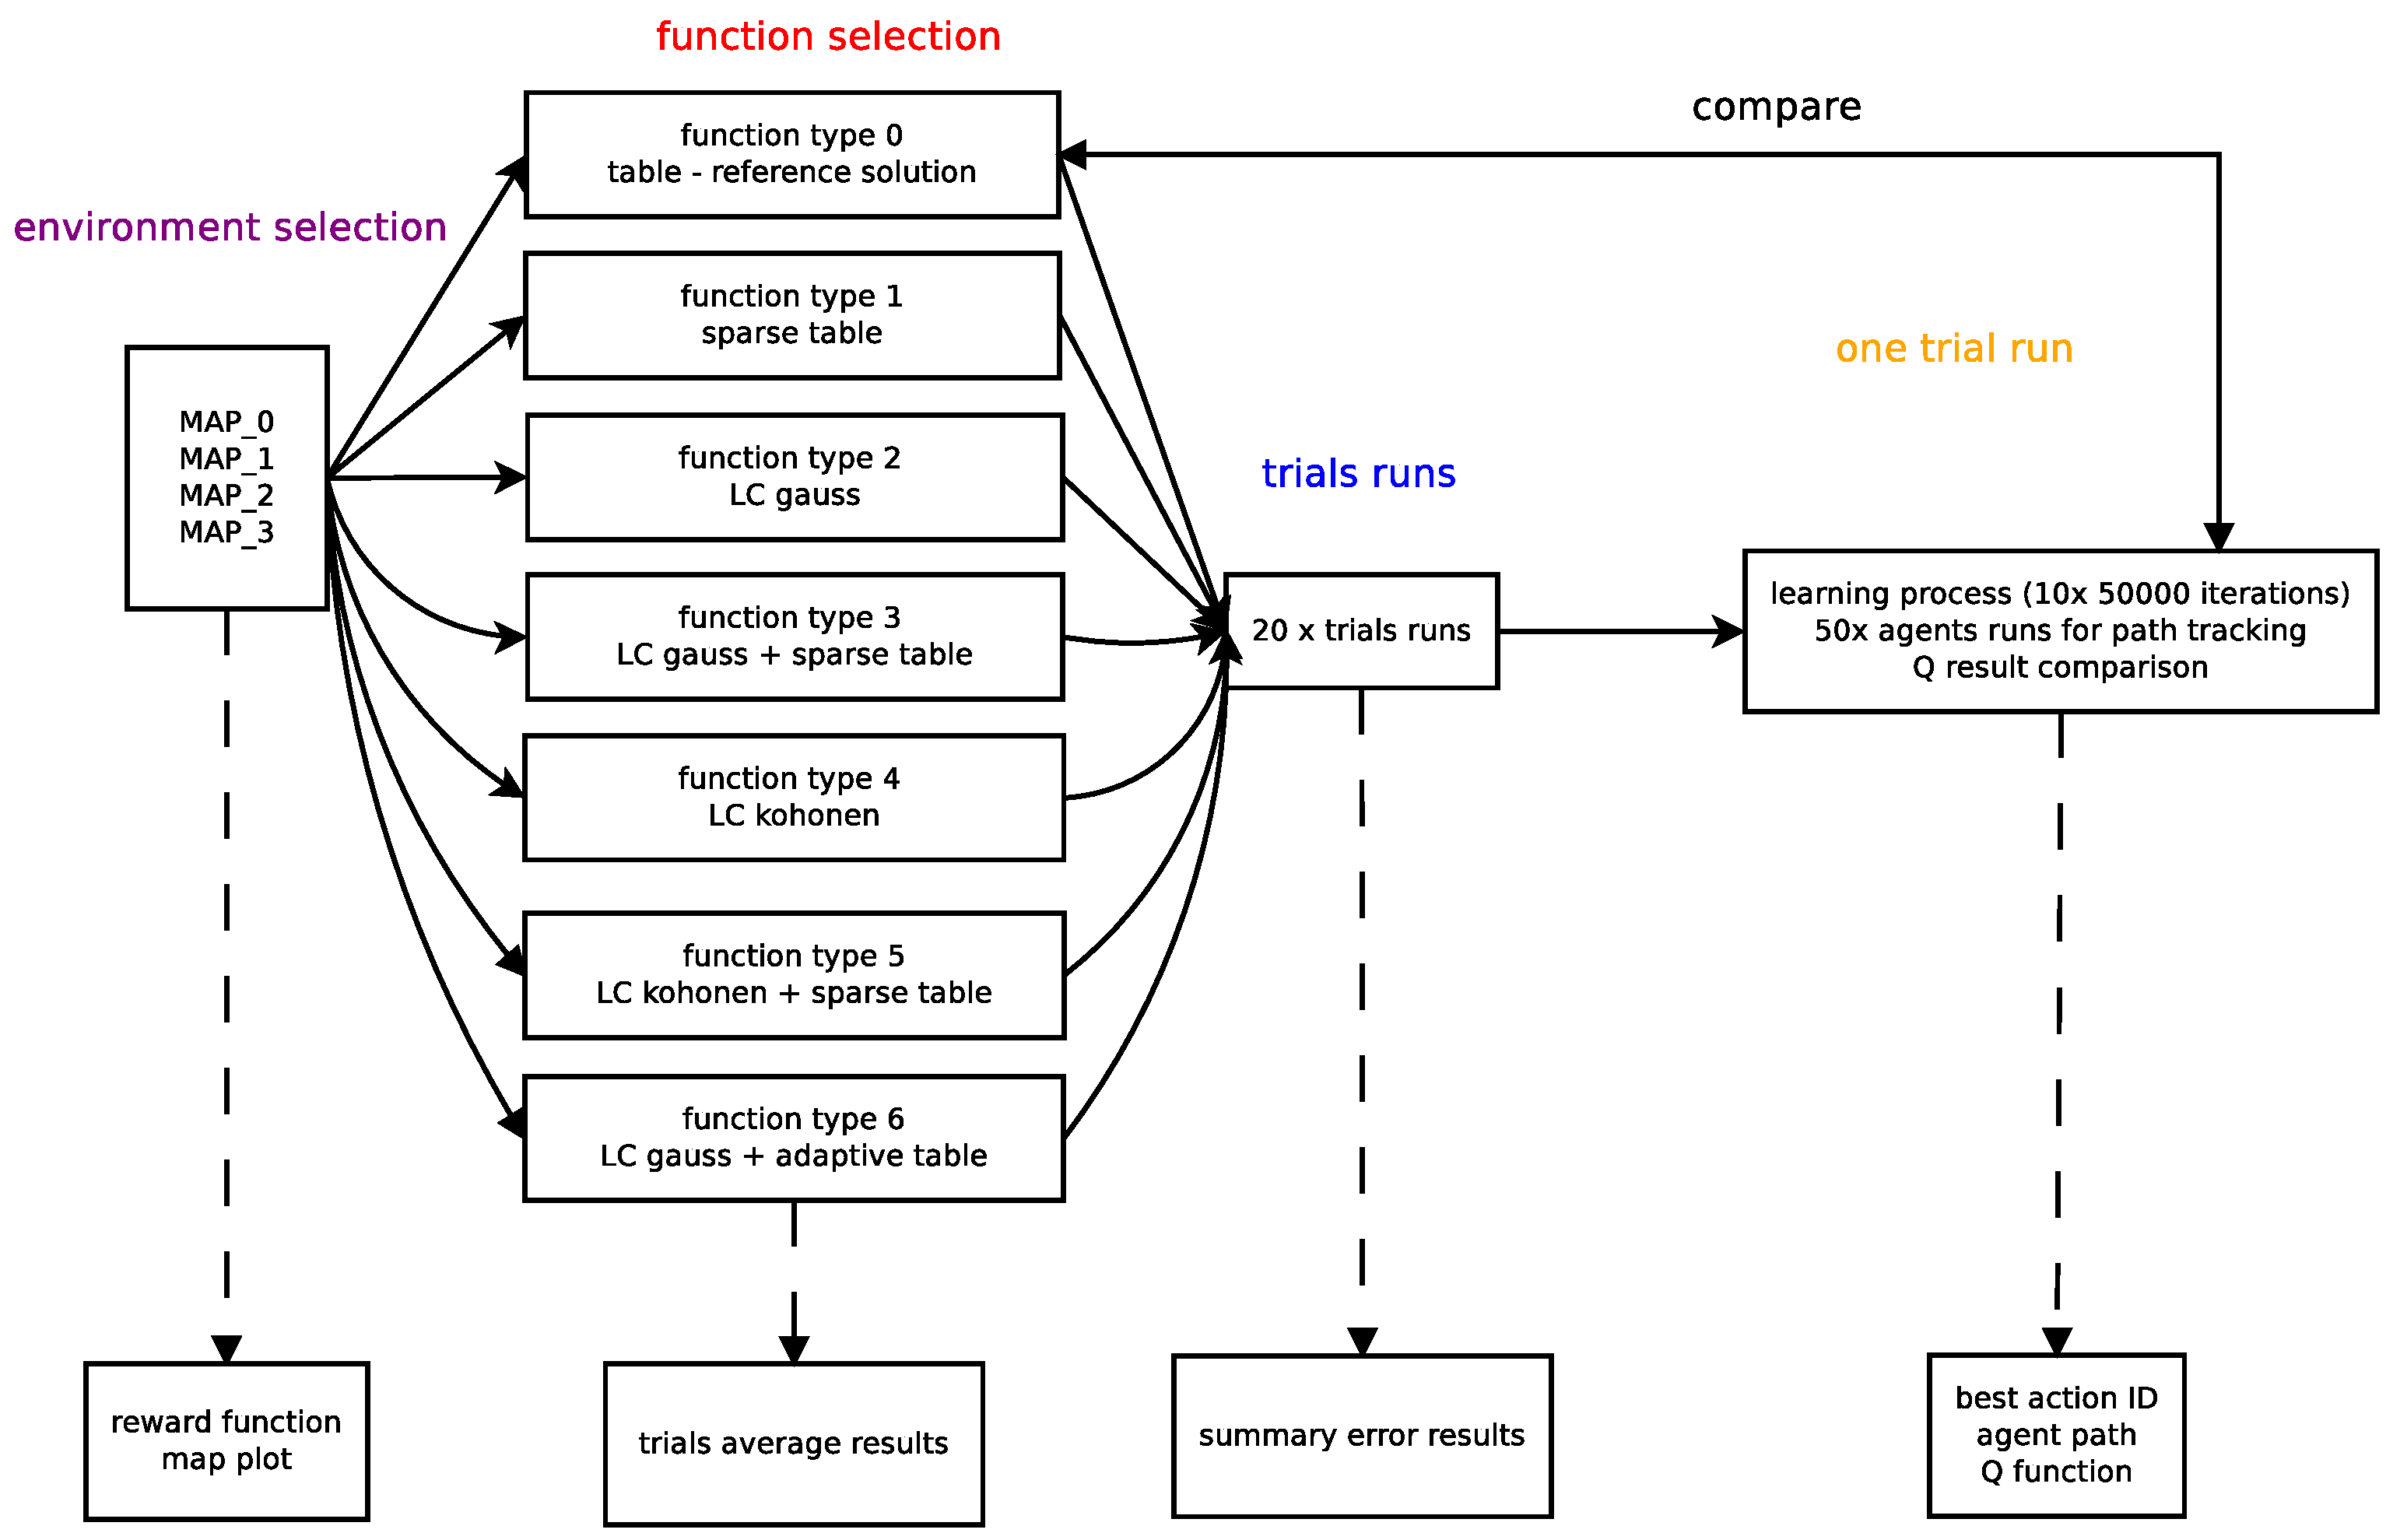
\includegraphics[scale=.3]{../diagrams/experiment_map_q_learning.eps}
\caption{Schéma experimentu}
\label{img:experiment_schem}
\end{figure}

Súhrnná schéma behu experimentov je na obrázku \ref{img:experiment_schem}.
Plné šípky predstavujú prepojenie úrovni metodológie. Čiarkované šípky znázorňujú
výstupy v jednotlivých úrovniach. Presné riešenie je použité na porovnanie výslednej chyby.



\begin{itemize}
\item 50000 iterácií učenia
\item rozmer $s$ je $n_s = 2$, rozmer $a$ je $n_a = 2$
\item predpis funkcie ohodnotení
\begin{align}
&Q(s(n),a(n)) = \nonumber \\
&\alpha Q(s(n-1),a(n-1)) \nonumber \\
&(1- \alpha)(R(s(n),a(n)) + \gamma \max_{a(n-1) \in \mathbb{A}} Q(s(n-1), a(n-1)) \nonumber
\end{align}

\item $R(s(n), a(n)) \in \langle -1, 1 \rangle$ náhodná mapa s 1 cieľovým stavom
\item $\gamma = 0.98$ a $\alpha = 0.7$
\item hustota referenčného riešenia = 1/32  (4096 stavov)
\item počet akcií v každom stave = 8
\item hustota riedkej tabuľky = 1/8  (1:16 pomer)
\item počet bázických funkcií $l = 64$
\item rozsah parametrov
    \begin{itemize}
      \item $\alpha_{ja}(n) \in \langle -1, 1 \rangle$
      \item $\beta_{ja}(n) \in \langle 0, 200 \rangle$
      \item $w_{ja}(n) \in \langle -4, 4 \rangle$
    \end{itemize}
\end{itemize}

$Q_{rt}(s(n),a(n))$ referenčná funkcia Q (funkcia 0), kde $t \in \langle 0, 19 \rangle $ je číslo trialu  \\
$Q_{jt}(s(n),a(n))$ testované funkcie Q a $j \in \langle 1, 5 \rangle $. \\

Celková chyba behu trialu $t$ je \\
\begin{equation}
e_{jt} = \sum\limits_{s, a}{(Q_{rt}(s,a) - Q_{jt}(s,a))^2}  \nonumber
\end{equation}

priemerná, minimálna, maximálna chyba a smerodatná odchylka \\
\begin{align}
\bar{a_j} &= \frac{1}{20}\sum\limits_{t}{e_{jt}}  \nonumber \\
{e^{min}_j} &= \min_{t}{e_{jt}}  \nonumber \\
{e^{max}_j} &= \max_{t}{e_{jt}}  \nonumber \\
{\sigma_j}^2 &= \frac{1}{20}\sum\limits_{t}{(\bar{a_j} - e_{jt})^2}  \nonumber
\end{align}

\section {Výsledky experimentu}



\begin{figure}[!htb]
\centering
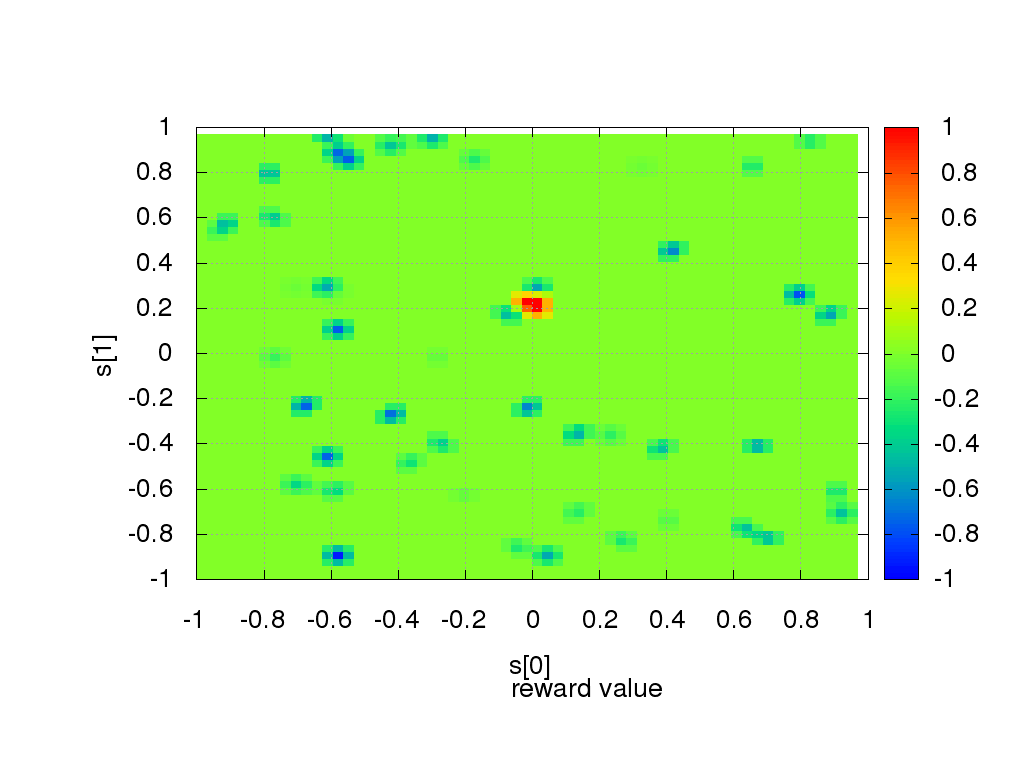
\includegraphics[scale=.4]{../../results_q_learning/map_1/reward_value_surface.png}
\caption{odmeňovacia funkcia}
\end{figure}



\begin{figure}[!htb]
\centering
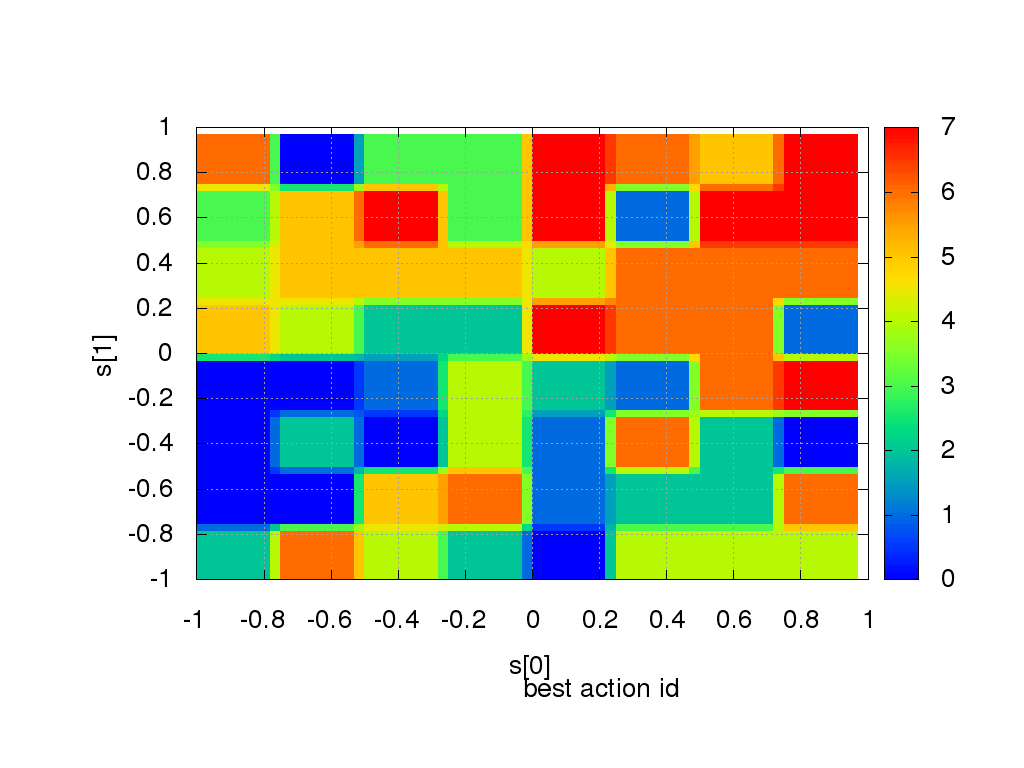
\includegraphics[scale=.4]{../../results_q_learning/map_1/function_type_1/iterations_10/action_best_value_log_surface.png}
\caption{fig:sparse table}
\end{figure}

\begin{figure}[!htb]
\centering
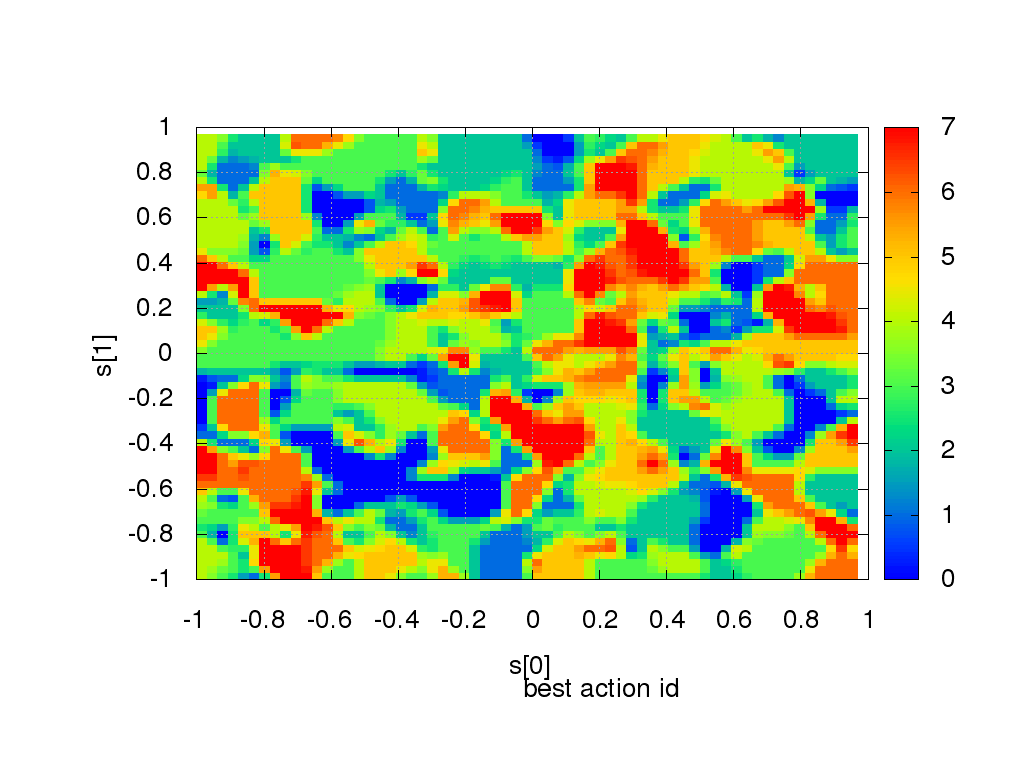
\includegraphics[scale=.4]{../../results_q_learning/map_1/function_type_2/iterations_10/action_best_value_log_surface.png}
\caption{fig:linear combination Gauss}
\end{figure}




\begin{figure}[!htb]
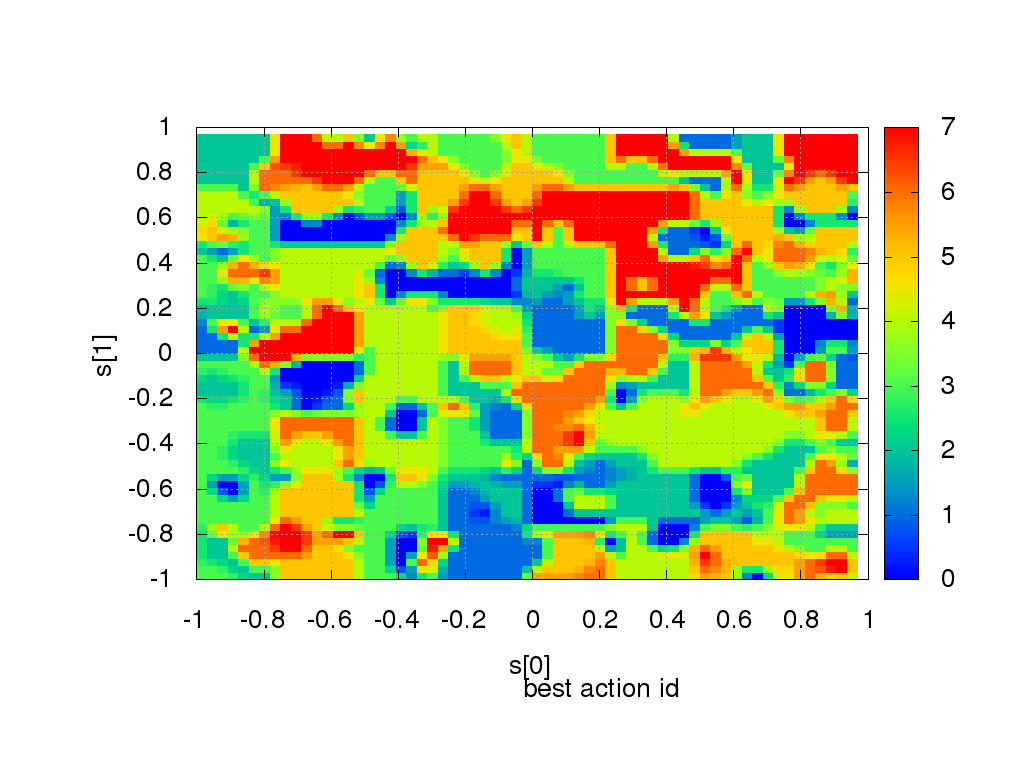
\includegraphics[scale=.4]{../../results_q_learning/map_1/function_type_3/iterations_10/action_best_value_log_surface.png}
\caption{sparse table + linear combination Gauss}
\end{figure}


\begin{figure}[!htb]
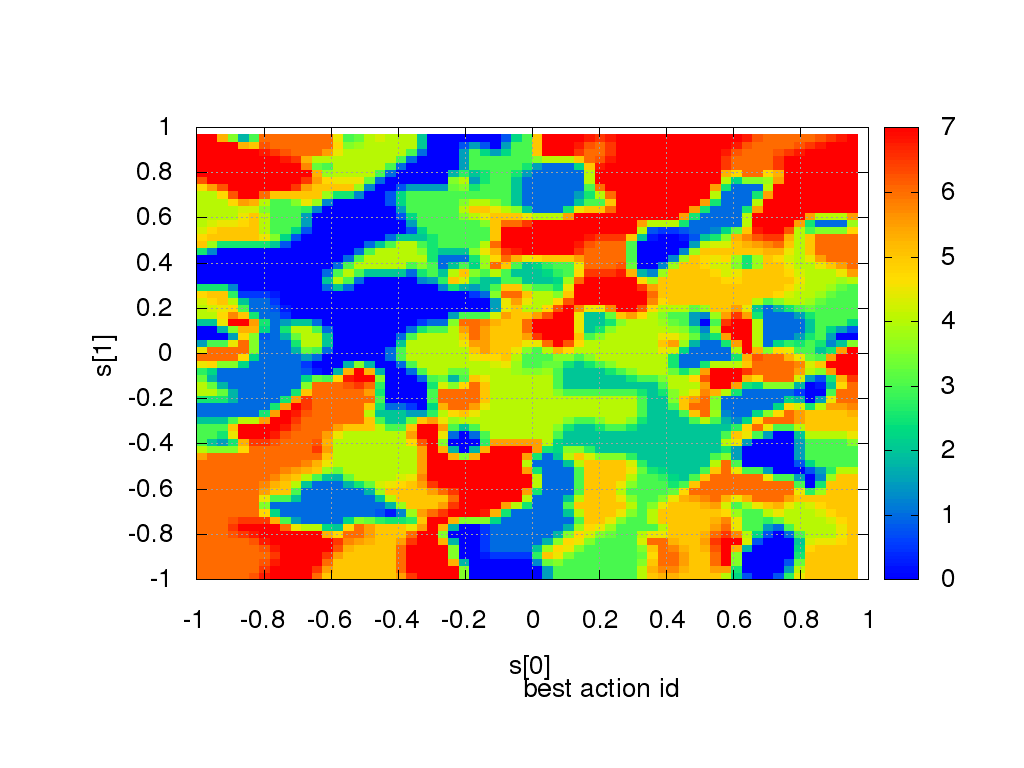
\includegraphics[scale=.4]{../../results_q_learning/map_1/function_type_4/iterations_10/action_best_value_log_surface.png}
\caption{linear combination Kohonen function}
\end{figure}




\begin{equation}
e_{jt}(s) = (Q_{rt}(s,a - Q_{jt}(s,a))^2  \nonumber
\end{equation}


\begin{figure}[!htb]
\centering
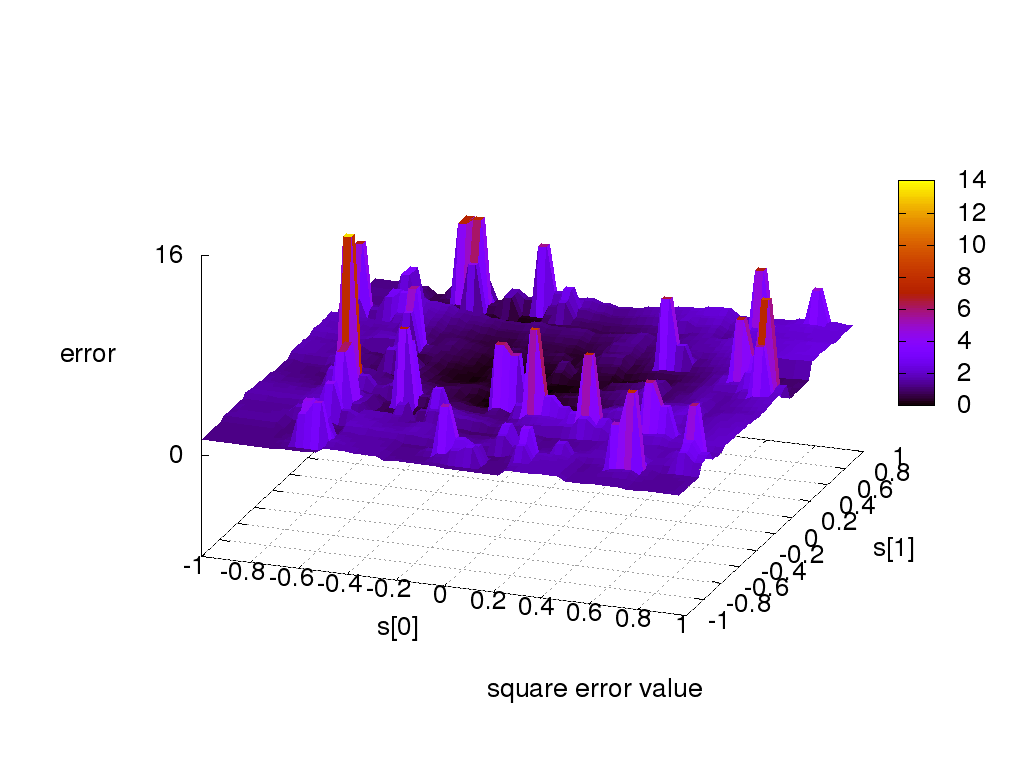
\includegraphics[scale=.4]{../../results_q_learning/map_1/function_type_1/q_learning_error.png}
\caption{sparse table}
\end{figure}


\begin{figure}[!htb]
\centering
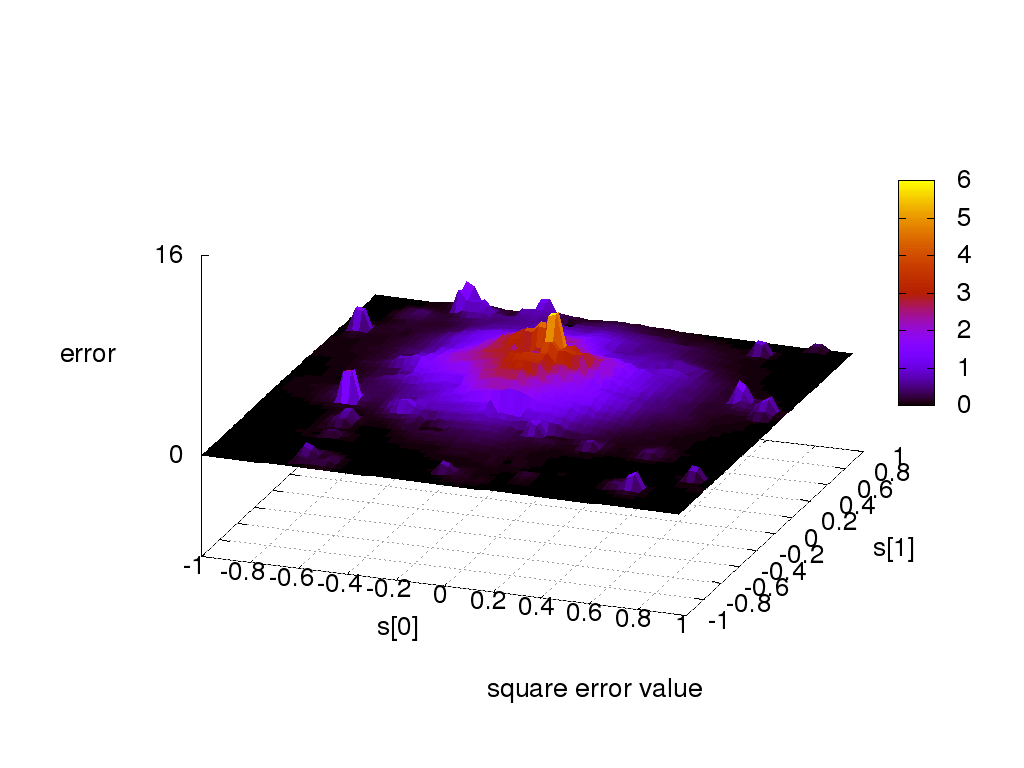
\includegraphics[scale=.4]{../../results_q_learning/map_1/function_type_2/q_learning_error.png}
\caption{linear combination Gauss}
\end{figure}



Chybové funkcie - Výsledky experimentov

\begin{equation}
e_{jt}(s) = (Q_{rt}(s,a - Q_{jt}(s,a))^2  \nonumber
\end{equation}

\begin{figure}[!htb]
\centering
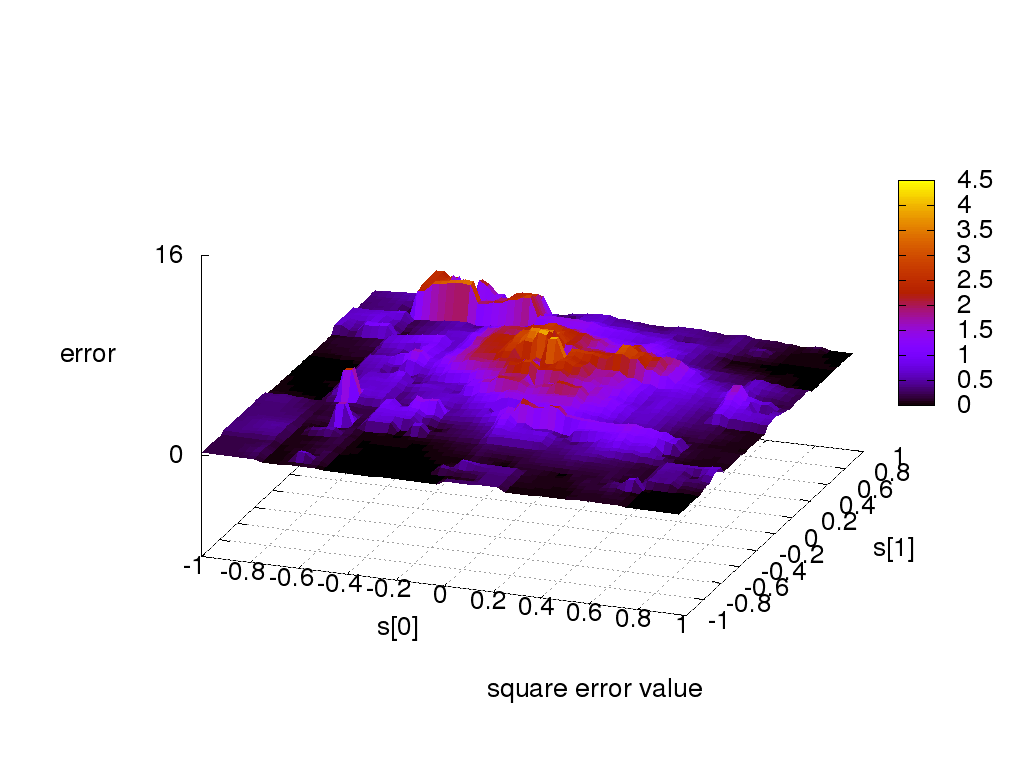
\includegraphics[scale=.4]{../../results_q_learning/map_1/function_type_3/q_learning_error.png}
\caption{sparse table + linear combination Gauss}
\end{figure}



\begin{figure}[!htb]
\centering
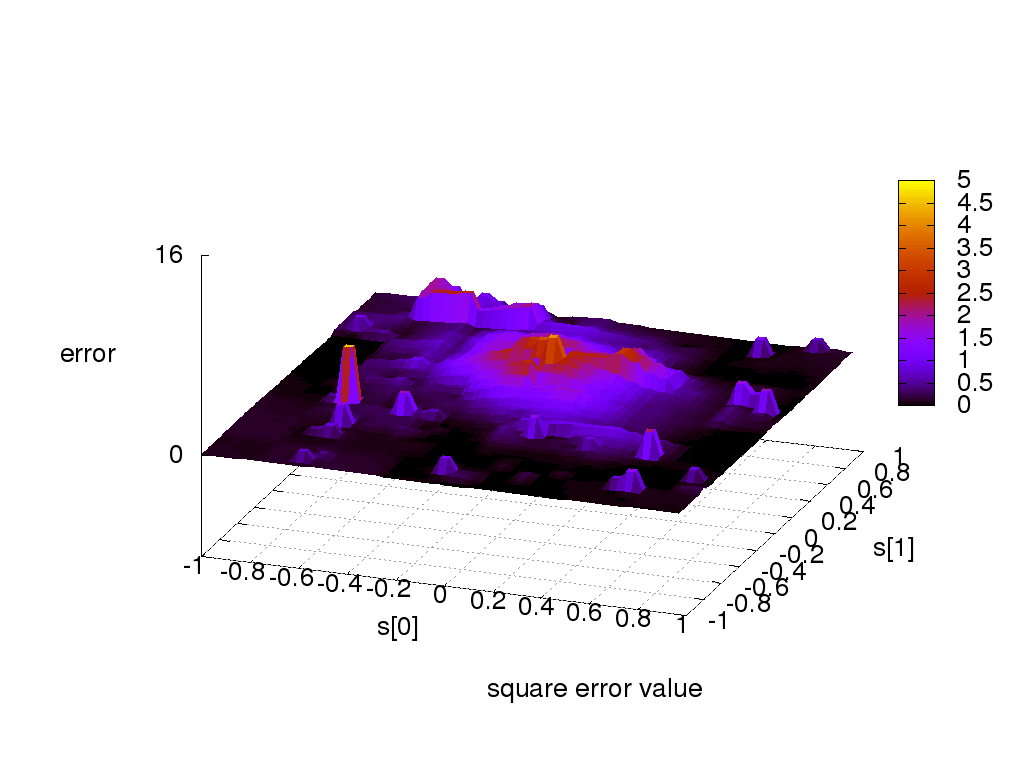
\includegraphics[scale=.4]{../../results_q_learning/map_1/function_type_4/q_learning_error.png}
\caption{linear combination Kohonen function}
\end{figure}






max Q(s, a) - Výsledky experimentov


\begin{figure}[!htb]
\centering
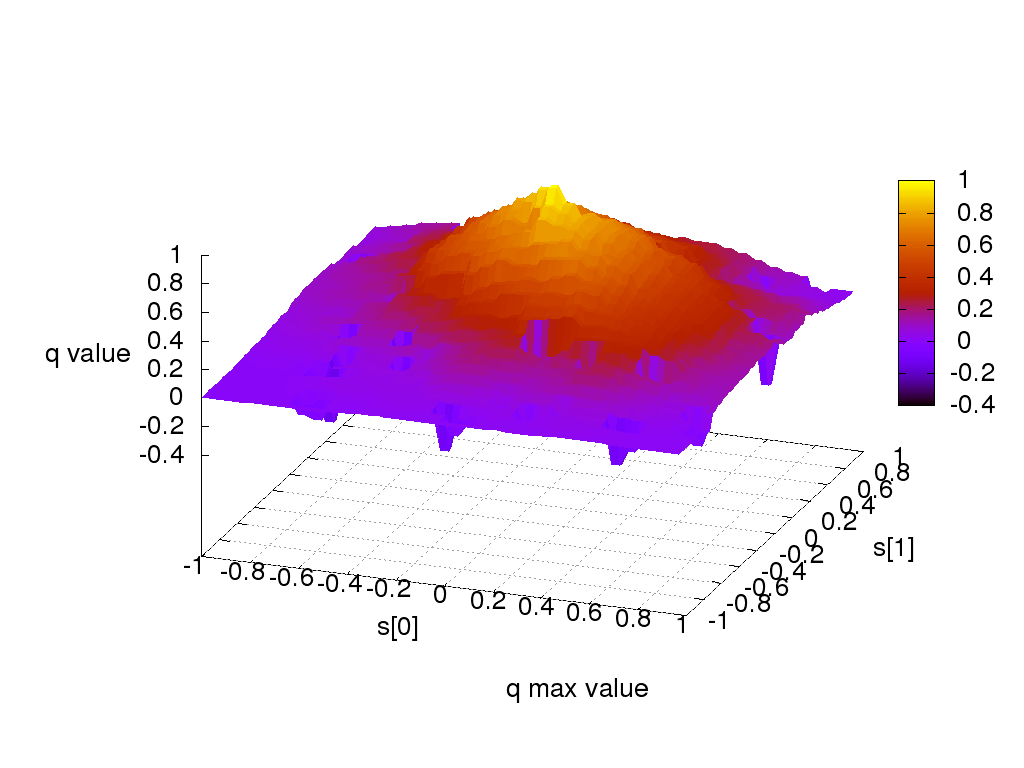
\includegraphics[scale=.4]{../../results_q_learning/map_1/function_type_0/iterations_10/q_learning_result.png}
\caption{reference table}
\end{figure}


\begin{figure}[!htb]
\centering
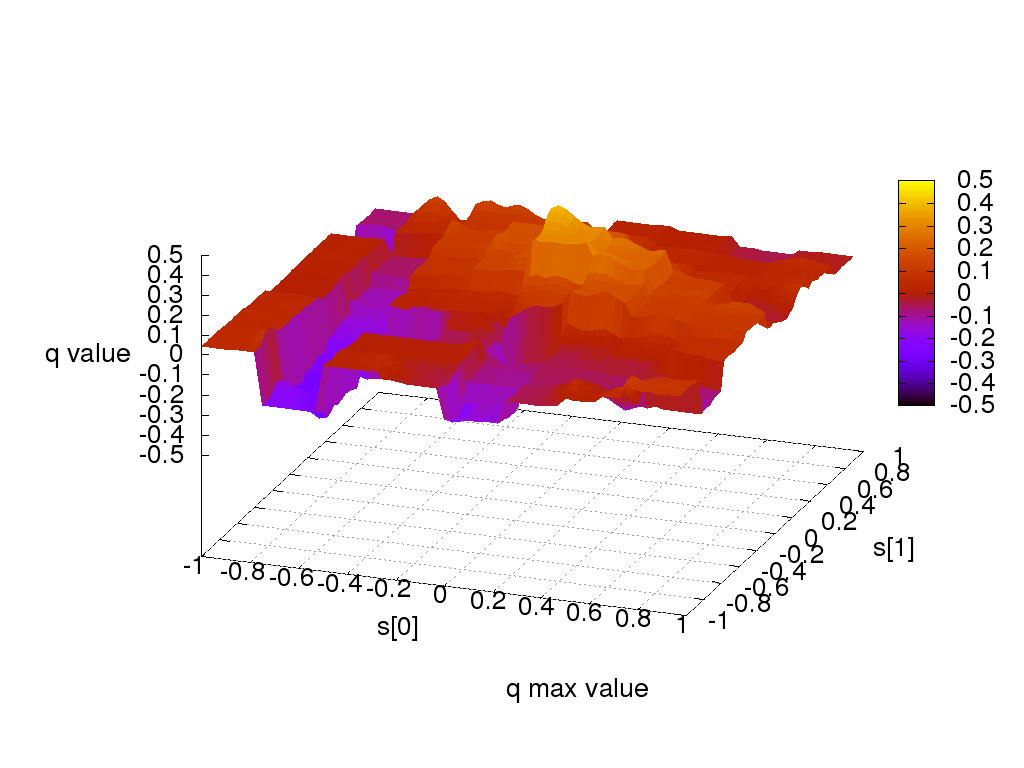
\includegraphics[scale=.4]{../../results_q_learning/map_1/function_type_3/iterations_10/q_learning_result.png}
\caption{sparse table + linear combination Gauss}
\end{figure}




Priebeh trialov - Výsledky experimentov

\begin{figure}[!htb]
\centering
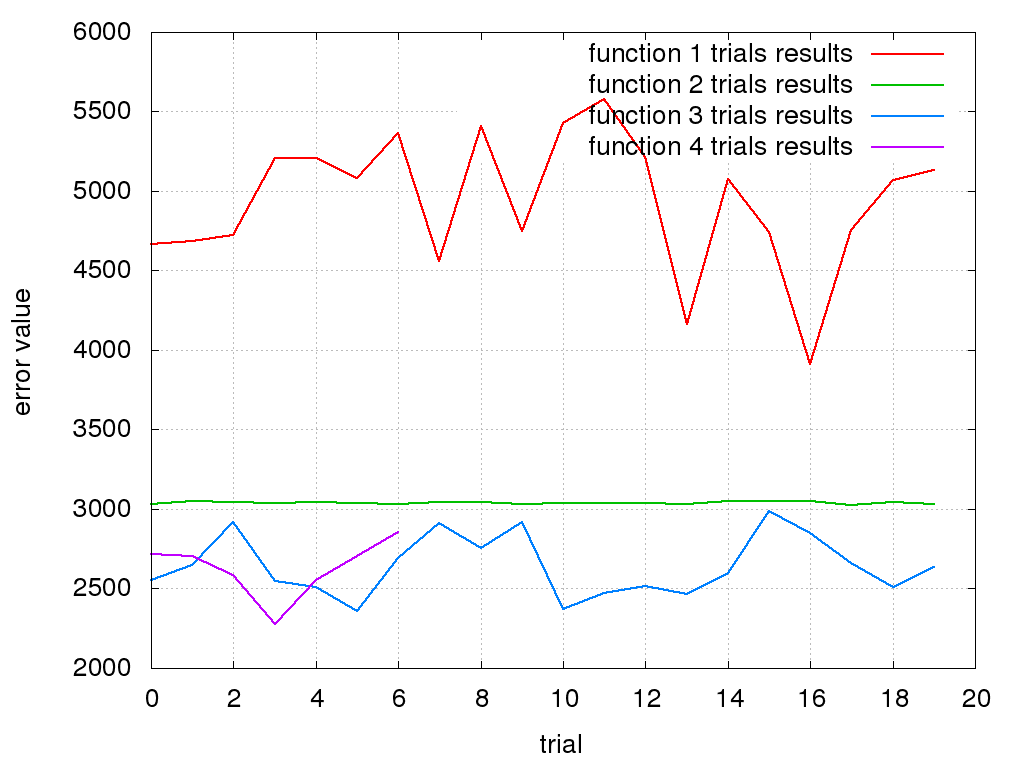
\includegraphics[scale=.4]{../../results_q_learning/map_1/trials_average_results_progress.png}
\end{figure}




Mapa 1 - Výsledky experimentov

\begin{figure}[!htb]
\centering
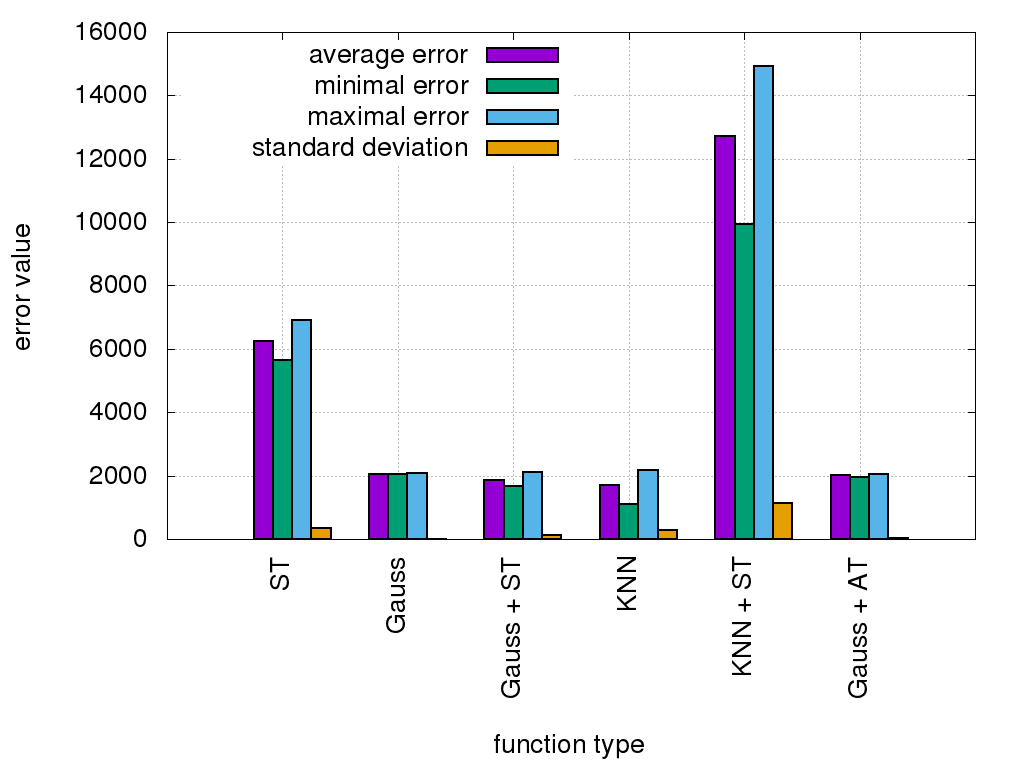
\includegraphics[scale=.4]{../../results_q_learning/map_1/trials_average_results.png}
\end{figure}



Mapa 0 - Výsledky experimentov

\begin{figure}[!htb]
\centering
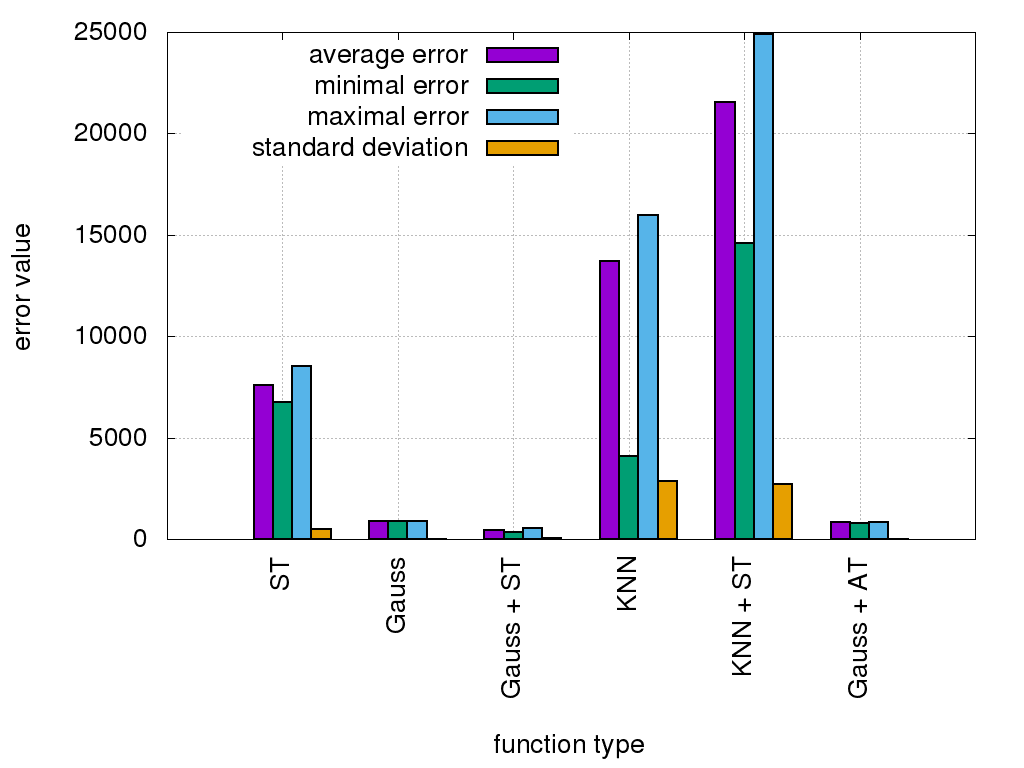
\includegraphics[scale=.4]{../../results_q_learning/map_0/trials_average_results.png}
\end{figure}


Mapa 2 - Výsledky experimentov

\begin{figure}[!htb]
\centering
\includegraphics[scale=.4]{../../results_q_learning/map_2/trials_average_results.png}
\end{figure}


Mapa 3 - Výsledky experimentov

\begin{figure}[!htb]
\centering
\includegraphics[scale=.4]{../../results_q_learning/map_3/trials_average_results.png}
\end{figure}

%\chapter{Záver}

Práca rieši problematiku aproximovania funkcie ohodnotení v algoritmoch Q-learning.
S pomedzi najčastejšie používaných prístupov bola zvolená aproximácia neurónovou
sieťou pomocou bázických funkcií. Oproti bežne používanému prístupu lineárnej kombinácií
príznakov (features) sa líši tým, že samotné tvary príznaky si algoritmus stanovuje sám,
počas učenia. Zmenšuje sa teda potrebná znalosť programátora.

{\bf Vedecký prínos} je možné nájsť v
\begin{itemize}
  \item Ukážka nevhodnosti použitia doprednej siete v predloženom probléme učenou
  gradientovými metódami. Riešenie nekonvergovalo ani po miliónoch iteráciach v triviálnom
  experimente s dvoma akciami. Príčinou je nelokálnosť učenia siete - zmena hodnoty v jednom bode,
  zmení hodnoty v každom bode, a nie nutne k lepšiemu. Od siete sa súčastne požaduje generovanie
  správnej hodnoty aj učenie v nejakom inom bode.
  \item Uvedenie algoritmu nanoQ, ktorý vyšetruje systém s jedným stavom. Nepodarilo sa nájsť
  publikáciu ktorá by tento princíp využívala. Algoritmus môže nájsť uplatnenie v riešení pohybu
  jednoduchého robota.
  \item Uvedenie novej bázickej funkcie, ktorá z testovaných najlepšie aproximuje funkciu ohodnotení.
  Táto funkcia môže byť učená lokálne, a vďaka časti $P(s(n), a(n))$ umožňuje zabezpečiť potrebnú
  strmosť, bez nutnosti širokého rozsahu parametrov $\beta$ v časti $H(s(n), a(n))$ - ten
  môže zostať malý, a riešiť tak šírenie kladnej odmeny na ďalšie stavy v súlade s parametrom
  $\gamma$.
  \item Testovanie Q-learing algoritmu na reálnom robotovi, kde predstavuje druhú úroveň
  riadenia. Na spodnej vrstve sa pravuje s PID regulátormi, na druhej sa pomocou Q-learning
  algoritmu stanovujú žiadané hodnoty.
\end{itemize}

Napriek uvedeným skutočnostiam a súčastnému stavu komerčnej sféry, autor práce nepredpokladá
využitie Q-learning algoritmov v priemyselnej praxi. Medzi hlavné dôvody možno zaradiť
konzervatívny prístup riadenia v priemysle, kde väčšinu úloh plnohodnotne vyrieši PID
regulátor a nad ním postavená logika vetvenia (napr. rôzne stavové automaty).
Práca tak predstavuje nepatrný prínos v teoretickej oblasti reinforcement learning algoritmov.
Jediné možné využitie v blízkej dobe je možné nájsť v počítačových hrách.
Všetky zdrojové súbory a podrobné výsledky experimentov (vrátane dát na ďalšie smerovanie)
sú k dispizícií pod GNU GPL licenciou. Práca tak spadá do kategórie otvorenej vedy.
Zdrojové súbory pre Q-learning experiment sú k dispozícií na autorovom gite \cite{bib:q_learning_git}.
Spolu je to cca 55648 súborov, z toho cca. 17000 pripadá na výsledky experimentov a cca 36000 na
 zdrojové súbory. Zdrojové súbory (vrátane podkladov na výrobu) pre robota Motoko sú k dispozícií na
 \cite{bib:motoko_git}.



%%%%%%%%%%%%%%%%%% literatura
%%%%%%%%%%%%%%%%%%%%%%%%%%%%%%%%%%%%%%%%%%%%%%%%%%%%%%%%%%%%%%%%%%%%%%%%%%%%%
\begin{thebibliography}{99}                                \label{literatura}
%\addcontentsline{toc}{section}{Literatúra}
\addcontentsline{toc}{chapter}{Literatúra}

\bibitem{bib:adaptive_01} Nhan Nguyen, NASA Ames Research Center, Moffett Field, CA 94035 :
Predictor-Model-Based Least-Squares Model-Reference Adaptive Control with Chebyshev Orthogonal Polynomial Approximation

\bibitem{bib:adaptive_02} Girish Chowdhary and Eric Johnson, Least  Squares  Based  Modification  for  Adaptive  Control
\url{http://web.mit.edu/girishc/www/publications/files/Chow_Joh_CDC_10_ls.pdf}

\bibitem{bib:adaptive_03}
Sun Pei, Noise Resistant Least Squares Based Adaptive Control, March 27, 2012, Stockholm, Sweden
\url{http://www.diva-portal.org/smash/get/diva2:514116/FULLTEXT01.pdf}


\bibitem{bib:gradient_01} Prof. Nathan L. Gibson Department of Mathematics,
Gradient-based Methods for Optimization. Part I., 2011
\url{http://math.oregonstate.edu/~gibsonn/optpart1.pdf}

\bibitem{bib:gradient_02} Antony Jameson,
Department of Aeronautics and Astronautics
Stanford University, Stanford, CA 94305-4035
Gradient Based Optimization Methods,
\url{http://aero-comlab.stanford.edu/Papers/jameson.gbom.pdf}

\bibitem{bib:gradient_03} L. Hasdorff, Gradient optimization and nonlinear control,
ISBN	0471358703, \url{https://books.google.cz/books?id=o\_ZQAAAAMAAJ}

\bibitem{bib:ilc_01} Kevin L. Moore, Iterative Learning Control,
\url{http://inside.mines.edu/~kmoore/survey.pdf}

\bibitem{bib:ilc_02}  Kevin L. Moore, An Introduction to Iterative Learning Control Theory,
\url{http://inside.mines.edu/~kmoore/504_ILC_Seminar-Save.pdf}

\bibitem{bib:gradient_04} Jeff Heaton, Introduction to Neural Networks with Java,
Heaton Research, Inc., 2008, ISBN	1604390085


\bibitem{bib:q_learning_watkins}
CHRISTOPHER  J.C.H. WATKINS, PETER DAYAN : Technical Note Q-Learning,
Machine Learning,  8,279-292 (1992)
\url{http://www.gatsby.ucl.ac.uk/~dayan/papers/cjch.pdf}

\bibitem{bib:q_tutorial_01} Q-learning 1
\url{https://www-s.acm.illinois.edu/sigart/docs/QLearning.pdf}

\bibitem{bib:q_tutorial_02} Q-learning 2
\url{http://mnemstudio.org/path-finding-q-learning-tutorial.htm}


\bibitem{bib:q_proof_01} Francisco S. Melo
Institute for Systems and Robotics,
Instituto Superior Técnico,
Lisboa, PORTUGAL : Convergence of Q-learning:  a simple proof
\url{http://users.isr.ist.utl.pt/~mtjspaan/readingGroup/ProofQlearning.pdf}

\bibitem{bib:q_proof_02} Eyal Even-Dar, Yishay Mansour :
Convergence of optimistic and incremental Q-learning,
\url{http://web.cs.iastate.edu/~honavar/rl-optimistic.pdf}


\bibitem{bib:q_proof_03}
Carden, Stephen, "Convergence of a Reinforcement Learning Algorithm in Continuous Domains" (2014).
All Dissertations. Paper 1325.
\url{http://tigerprints.clemson.edu/cgi/viewcontent.cgi?article=2326&context=all_dissertations}

\bibitem{bib:q_proof_04} Francisco S. Melo and M. Isabel Ribeiro,
Convergence of Q-learning with linear function approximation,
Proceedings of the European Control Conference 2007 Kos, Greece, July 2-5, 2007,
\url{http://gaips.inesc-id.pt/~fmelo/pub/melo07ecc.pdf}

\bibitem{bib:sarsa} Karan M. Gupta Department of Computer Science Texas TechUniversity Lubbock, TX 79409-3104 :
Performance Comparison of Sarsa($\lambda$) and Watkin’s Q($\lambda$) Algorithms,
\url{http://www.karanmg.net/Computers/reinforcementLearning/finalProject/KaranComparisonOfSarsaWatkins.pdf}


\bibitem{bib:kohonen_01} R. Rojas: Neural Networks, Springer-Verlag, Berlin, 1996, Kohonen Networks
\url{https://page.mi.fu-berlin.de/rojas/neural/chapter/K15.pdf}

\bibitem{bib:kohonen_02} Steven K. Rogers, Matthew Kabrisky
SPIE Press, 1991, ISBN	0819405345 : An Introduction to Biological and Artificial Neural Networks for Pattern Recognition
\url{https://books.google.cz/books?id=uo4Smk6QnTgC}

\bibitem{bib:kohonen_03} Teuvo Kohonen and Timo Honkela (2007), Scholarpedia, 2(1):1568 : Kohonen network
\url{http://www.scholarpedia.org/article/Kohonen_network}

\bibitem{bib:markov_01} Markovove rozhodovacie procesy, stručne :
Pieter Abbeel  UC Berkeley EECS : Markov Decision Processes and Exact Solution Methods
\url{http://www.cs.berkeley.edu/~pabbeel/cs287-fa12/slides/mdps-exact-methods.pdf}

\bibitem{bib:markov_02} Martin L. Puterman : Markov Decision Processes: Discrete Stochastic Dynamic Programming
, isbn 9781118625873, rok 2014, \url{https://books.google.sk/books?id=VvBjBAAAQBAJ}

\bibitem{bib:nano_q_link}
NanoQ learning zdrojové súbory \url{https://github.com/michalnand/q_learning/tree/master/src/nano_q_learning}

\bibitem{bib:kolomongorov_01}
Fundamentals of Artificial Neural Networks Mohamad H. Hassoun, MIT Press, 1995

\bibitem{bib:kolomongorov_02}
B. Irie Auditory \& Visual Perception Res. Lab., ATR, Osaka, Japan, S. Miyake :
Neural Networks, 1988., IEEE International Conference on, INSPEC 3350063

\bibitem{bib:kolomongorov_03}
Kolomongorov teorém, stručne
\url{https://en.wikipedia.org/wiki/Universal_approximation_theorem}

\bibitem{bib:backpropagation_00}
R. Rojas: Neural Networks, Springer-Verlag, Berlin, 1996, chap 7

\bibitem{bib:backpropagation_01}
Martin Riedmiller,  Computer Standards \& Interfaces Volume 16, Issue 3, July 1994, Pages 265-278 :
Advanced supervised learning in multi-layer perceptrons — From backpropagation to adaptive learning algorithms

\bibitem{bib:backpropagation_02}
J. Leonard, M.A. Kramer, Computers \& Chemical Engineering Volume 14, Issue 3, March 1990, Pages 337–341
Improvement of the backpropagation algorithm for training neural networks

\bibitem{bib:annealing_01} Jonathan Engel,
Norman Bridge Laboratoryof Plly sics 161-33, California Institute of Technology,
Pasadena, CA 91125, USA : Teaching Feed-Forward Neural Networks by Simulated Annealing



\bibitem{bib:aproximation_01} Francisco S. Melo, Sean P. Meyn, M. Isabel Ribeiro
An Analysis of Reinforcement Learning with Function Approximation,
Appearing in Proceedings of the 25th International Conference on Machine Learning, Helsinki, Finland, 2008
\url{http://www.machinelearning.org/archive/icml2008/papers/652.pdf}

\bibitem{bib:aproximation_02} David Silver : Lecture 6: Value Function Approximation
\url{http://www0.cs.ucl.ac.uk/staff/d.silver/web/Teaching_files/FA.pdf}

\bibitem{bib:aproximation_03} Francisco S. Melo M. Isabel Ribeiro : Q-learning with linear function approximation
\url{http://gaips.inesc-id.pt/~fmelo/pub/melo07tr-b.pdf}

\bibitem{bib:aproximation_04} Marina Irodova and Robert H. Sloan : Reinforcement Learning and Function Approximation,
2005,  American  Association  for  Artificial  Intelli-gence (www.aaai.org)
\url{http://citeseerx.ist.psu.edu/viewdoc/download?doi=10.1.1.81.7833&rep=rep1&type=pdf}



\bibitem{bib:strategy_01} Punit Pandey, Dr. Shishir Kumar, DeepshikhaPandey,
Reinforcement Learning by Comparing Immediate Reward, (IJCSIS)
International Journal of Computer Science and Information Security, Vol. 8
, No. 5, August 2010
\url{http://arxiv.org/pdf/1009.2566.pdf}

\bibitem{bib:strategy_02} Melanie Coggan, CRA-W DMP Project at McGill University (2004) :
Exploration and Exploitation inReinforcement Learning
\url{http://ftp.bstu.by/ai/To-dom/My_research/Papers-2.1-done/RL/0/FinalReport.pdf}

\bibitem{bib:strategy_03} Mark Humphrys Trinity Hall, University of Cambridge August 1996,
\url{http://citeseerx.ist.psu.edu/viewdoc/download?doi=10.1.1.73.8309&rep=rep1&type=pdf}

\bibitem{bib:q_app_01}
Jinyi Yao Dept. of Comput. Sci. \& Technol., Tsinghua Univ., Beijing, China Jiang Chen ; Zengqi Sun
An application in RoboCup combining Q-learning with adversarial planning, 2002
\url{http://ieeexplore.ieee.org/xpl/freeabs_all.jsp?arnumber=1022159&abstractAccess=no&userType=inst}


\bibitem{bib:q_app_02} Asma Al-Tamimi, Frank L. Lewis , Murad Abu-Khalaf
Model-free Q-learning designs for linear discrete-time zero-sum games with application to H-infinity control, 2006
\url{http://www.sciencedirect.com/science/article/pii/S0005109806004249}

\bibitem{bib:q_app_03} Asma Al-Tamimi, Frank L. Lewis , Murad Abu-Khalaf
Model-free Q-learning designs for linear discrete-time zero-sum games with application to H-infinity control, 2006
\url{http://www.sciencedirect.com/science/article/pii/S0005109806004249}

\bibitem{bib:q_conv_proof}
Christopher J. C. H. Watkins, Peter Dayan
Q-learning, 1992
\url{http://link.springer.com/article/10.1007/BF00992698}

\bibitem{bib:q_fnn_problem}
Mae L. Seto Springer Science \& Business Media, 9. 12. 2012,
Marine Robot Autonomy, ISBN	1461456592, chap 7.3.3.2

\bibitem{bib:reinforcement_leraning_01}
Peter Dayan, Christopher J.C.H. Watkins,
Reinforcement Learning
\url{http://www.gatsby.ucl.ac.uk/~dayan/papers/dw01.pdf}


\bibitem{bib:reinforcement_leraning_02}
Daniel Dewey, Oxford Martin Programme on the Impacts of Future Technology,
Future of Humanity Institute :
Reinforcement Learning and the Reward Engineering Principle
\url{http://www.danieldewey.net/reward-engineering-principle.pdf}

\bibitem{bib:mototko_video} video robota Motoko Aftermath
Michal Chovanec, youtube
\url{https://www.youtube.com/watch?v=8sskJN_zuko}

\bibitem{bib:q_learning_git} Michal Chovanec, Q-learning zdrojové súbory \url{https://github.com/michalnand/q_learning}

\bibitem{bib:motoko_git} Michal Chovanec, Motoko robot zdrojové súbory \url{https://github.com/michalnand/motoko_after_math_linefollower}


\end{thebibliography}


\end{document}
